\documentclass[a4paper]{article}

\def\npart {IA}
\def\nterm {Michaelmas}
\def\nyear {2014}
\def\nlecturer {N.\ Peake}
\def\ncourse {Vectors and Matrices}

\usepackage{myheader}

\begin{document}
\maketitle
{\small \noindent\textbf{Complex numbers}\\
Review of complex numbers, including complex conjugate, inverse, modulus, argument and Argand diagram. Informal treatment of complex logarithm, $n$-th roots and complex powers. de Moivre's theorem.\hspace*{\fill}[2]

\vspace{10pt}
\noindent\textbf{Vectors}\\
Review of elementary algebra of vectors in $\R^3$, including scalar product. Brief discussion of vectors in $\R^n$ and $\C^n$; scalar product and the Cauchy-Schwarz inequality. Concepts of linear span, linear independence, subspaces, basis and dimension.

\vspace{5pt}
\noindent Suffix notation: including summation convention, $\delta_{ij}$ and $\varepsilon_{ijk}$. Vector product and triple product: definition and geometrical interpretation. Solution of linear vector equations. Applications of vectors to geometry, including equations of lines, planes and spheres.\hspace*{\fill}[5]

\vspace{10pt}
\noindent\textbf{Matrices}\\
Elementary algebra of $3\times 3$ matrices, including determinants. Extension to $n\times n$ complex matrices. Trace, determinant, non-singular matrices and inverses. Matrices as linear transformations; examples of geometrical actions including rotations, reflections, dilations, shears; kernel and image.\hspace*{\fill}[4]

\vspace{5pt}
\noindent Simultaneous linear equations: matrix formulation; existence and uniqueness of solutions, geometric interpretation; Gaussian elimination.\hspace*{\fill}[3]

\vspace{5pt}
\noindent Symmetric, anti-symmetric, orthogonal, hermitian and unitary matrices. Decomposition of a general matrix into isotropic, symmetric trace-free and antisymmetric parts.\hspace*{\fill}[1]

\vspace{10pt}
\noindent\textbf{Eigenvalues and Eigenvectors}\\
Eigenvalues and eigenvectors; geometric significance.\hspace*{\fill}[2]

\vspace{5pt}
\noindent Proof that eigenvalues of hermitian matrix are real, and that distinct eigenvalues give an orthogonal basis of eigenvectors. The effect of a general change of basis (similarity transformations). Diagonalization of general matrices: sufficient conditions; examples of matrices that cannot be diagonalized. Canonical forms for $2 \times 2$ matrices.\hspace*{\fill}[5]

\vspace{5pt}
\noindent Discussion of quadratic forms, including change of basis. Classification of conics, cartesian and polar forms.\hspace*{\fill}[1]

\vspace{5pt}
\noindent Rotation matrices and Lorentz transformations as transformation groups.\hspace*{\fill}[1]}

\tableofcontents

\setcounter{section}{-1}
\section{Introduction}
Vectors and matrices is the language in which a lot of mathematics is written in. In physics, many variables such as position and momentum are expressed as vectors. Heisenberg also formulated quantum mechanics in terms of vectors and matrices. In statistics, one might pack all the results of all experiments into a single vector, and work with a large vector instead of many small quantities. In group theory, matrices are used to represent the symmetries of space (as well as many other groups).

So what is a vector? Vectors are very general objects, and can in theory represent very complex objects. However, in this course, our focus is on vectors in $\R^n$ or $\C^n$. We can think of each of these as an array of $n$ real or complex numbers. For example, $(1, 6, 4)$ is a vector in $\R^3$. These vectors are added in the obvious way. For example, $(1, 6, 4) + (3, 5, 2) = (4, 11, 6)$. We can also multiply vectors by numbers, say $2(1, 6, 4) = (2, 12, 8)$. Often, these vectors represent points in an $n$-dimensional space.

Matrices, on the other hand, represent \emph{functions} between vectors, i.e.\ a function that takes in a vector and outputs another vector. These, however, are not arbitrary functions. Instead matrices represent \emph{linear functions}. These are functions that satisfy the equality $f(\lambda \mathbf{x} + \mu \mathbf{y}) = \lambda f(\mathbf{x}) + \mu f(\mathbf{y})$ for arbitrary numbers $\lambda, \mu$ and vectors $\mathbf{x}, \mathbf{y}$. It is important to note that the function $\mathbf{x} \mapsto \mathbf{x} + \mathbf{c}$ for some constant vector $\mathbf{c}$ is \emph{not} linear according to this definition, even though it might look linear.

It turns out that for each linear function from $\R^n$ to $\R^m$, we can represent the function uniquely by an $m\times n$ array of numbers, which is what we call the \emph{matrix}. Expressing a linear function as a matrix allows us to conveniently study many of its properties, which is why we usually talk about matrices instead of the function itself.

\section{Complex numbers}
In $\R$, not every polynomial equation has a solution. For example, there does not exist any $x$ such that $x^2 + 1 = 0$, since for any $x$, $x^2$ is non-negative, and $x^2 + 1$ can never be $0$. To solve this problem, we introduce the ``number'' $i$ that satisfies $i^2 = -1$. Then $i$ is a solution to the equation $x^2 + 1 = 0$. Similarly, $-i$ is also a solution to the equation.

We can add and multiply numbers with $i$. For example, we can obtain numbers $3 + i$ or $1 + 3i$. These numbers are known as \emph{complex numbers}. It turns out that by adding this single number $i$, \emph{every} polynomial equation will have a root. In fact, for an $n$th order polynomial equation, we will later see that there will always be $n$ roots, if we account for multiplicity. We will go into details in Chapter~\ref{sec:eigen}.

Apart from solving equations, complex numbers have a lot of rather important applications. For example, they are used in electronics to represent alternating currents, and form an integral part in the formulation of quantum mechanics.

\subsection{Basic properties}
\begin{defi}[Complex number]
  A \emph{complex number} is a number $z\in \C$ of the form $z = a + ib$ with $a, b\in \R$, where $i^2=-1$. We write $a = \Re(z)$ and $b = \Im(z)$.
\end{defi}

We have
\begin{align*}
  z_1\pm z_2 &= (a_1 + ib_1)\pm (a_2 + ib_2)\\
  &= (a_1\pm a_2) + i(b_1 \pm b_2)\\
  z_1z_2 &= (a_1 + ib_1)(a_2 + ib_2)\\
  &= (a_1a_2 - b_1b_2) + i(b_1a_2 + a_1b_2)\\
  z^{-1} &= \frac{1}{a + ib}\\
  &= \frac{a - ib}{a^2 + b^2}
\end{align*}
\begin{defi}[Complex conjugate]
  The \emph{complex conjugate} of $z = a+ ib$ is $a - ib$. It is written as $\bar{z}$ or $z^*$.
\end{defi}

It is often helpful to visualize complex numbers in a diagram:
\begin{defi}[Argand diagram]
  An \emph{Argand diagram} is a diagram in which a complex number $z = x + iy$ is represented by a vector $\mathbf{p}=\begin{pmatrix}x\\y\end{pmatrix}$. Addition of vectors corresponds to vector addition and $\bar{z}$ is the reflection of $z$ in the $x$-axis.
\begin{center}
  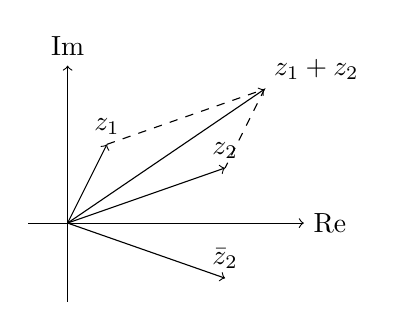
\begin{tikzpicture}
    \draw [->] (-0.5, 0) -- (3, 0) node [right] {Re};
    \draw [->] (0, -1) -- (0, 2) node [above] {Im};
    \draw [->] (0, 0) -- (.5, 1) node [above] {$z_1$};
    \draw [->] (0, 0) -- (2, .7) node [above] {$z_2$};
    \draw [->] (0, 0) -- (2, -.7) node [above] {$\bar z_2$};
    \draw [->] (0, 0) -- (2.5, 1.7) node [anchor=south west] {$z_1 + z_2$};
    \draw [dashed] (.5, 1) -- (2.5, 1.7) -- (2, .7);
  \end{tikzpicture}
\end{center}
\end{defi}

\begin{defi}[Modulus and argument of complex number]
  The \emph{modulus} of $z = x + iy$ is $r = |z| = \sqrt{x^2 + y^2}$. The \emph{argument} is $\theta = \arg z = \tan^{-1} (y/x)$. The modulus is the length of the vector in the Argand diagram, and the argument is the angle between $z$ and the real axis. We have
  \[
    z = r(\cos\theta + i\sin \theta)
  \]
  Clearly the pair $(r, \theta)$ uniquely describes a complex number $z$, but each complex number $z\in \C$ can be described by many different $\theta$ since $\sin (2\pi + \theta) = \sin \theta$ and $\cos(2\pi + \theta) = \cos\theta$. Often we take the \emph{principle value} $\theta \in (-\pi, \pi]$.
\end{defi}

When writing $z_i = r_i(\cos\theta_i + i\sin \theta_i)$, we have
\begin{align*}
  z_1z_2 &= r_1r_2[(\cos\theta_1\cos\theta_2 - \sin\theta_1\sin\theta_2) + i(\sin\theta_1\cos\theta_2 + \sin\theta_2\cos\theta_1)]\\
  &= r_1r_2[\cos(\theta_1 + \theta_2) + i\sin(\theta_1+\theta_2)]
\end{align*}
In other words, when multiplying complex numbers, the moduli multiply and the arguments add.

\begin{prop}
  $z\bar{z} = a^2 + b^2 = |z|^2$.
\end{prop}

\begin{prop}
  $z^{-1} = \bar{z}/|z|^2$.
\end{prop}

\begin{thm}[Triangle inequality]
  For all $z_1, z_2 \in \C$, we have
  \[
    |z_1 + z_2| \leq |z_1| + |z_2|.
  \]
  Alternatively, we have $|z_1 - z_2|\geq ||z_1| - |z_2||$.
\end{thm}

\subsection{Complex exponential function}
Exponentiation was originally defined for integer powers as repeated multiplication. This is then extended to rational powers using roots. We can also extend this to any real number since real numbers can be approximated arbitrarily accurately by rational numbers. However, what does it mean to take an exponent of a complex number?

To do so, we use the Taylor series definition of the exponential function:
\begin{defi}[Exponential function]
  The \emph{exponential function} is defined as
  \[
    \exp (z) = e^z = 1 + z + \frac{z^2}{2!} + \frac{z^3}{3!} + \cdots = \sum_{n = 0}^\infty \frac{z^n}{n!}.
  \]
\end{defi}
This automatically allows taking exponents of arbitrary complex numbers. Having defined exponentiation this way, we want to check that it satisfies the usual properties, such as $\exp(z + w) = \exp(z)\exp(w)$. To prove this, we will first need a helpful lemma.

\begin{lemma}
  \[
    \sum_{n = 0}^\infty\sum_{m = 0}^\infty a_{mn} = \sum_{r = 0}^\infty\sum_{m = 0}^r a_{r - m, m}
  \]
\end{lemma}

\begin{proof}
  \begin{align*}
    \sum_{n = 0}^\infty\sum_{m = 0}^\infty a_{mn} &= a_{00} + a_{01} + a_{02} + \cdots\\
    &+ a_{10} + a_{11} + a_{12} + \cdots\\
    &+ a_{20} + a_{21} + a_{22} + \cdots\\
    &= (a_{00}) + (a_{10} + a_{01}) + (a_{20} + a_{11} + a_{02}) + \cdots\\
    &= \sum_{r = 0}^\infty\sum_{m = 0}^r a_{r - m, m} \qedhere
  \end{align*}
\end{proof}
This is not exactly a rigorous proof, since we should not hand-wave about infinite sums so casually. But in fact, we did not even show that the definition of $\exp(z)$ is well defined for all numbers $z$, since the sum might diverge. All these will be done in that IA Analysis I course.

\begin{thm}
  $\exp(z_1)\exp(z_2) = \exp(z_1 + z_2)$
\end{thm}

\begin{proof}
  \begin{align*}
    \exp(z_1)\exp(z_2) &= \sum_{n = 0}^\infty\sum_{m = 0}^\infty \frac{z_1^m}{m!}\frac{z_2^n}{n!}\\
    &= \sum_{r = 0}^\infty\sum_{m = 0}^r \frac{z_1^{r - m}}{(r - m)!}\frac{z_2^m}{m!}\\
    &= \sum_{r = 0}^\infty\frac{1}{r!}\sum_{m = 0}^r \frac{r!}{(r - m)!m!}z_1^{r - m}z_2^m\\
    &= \sum_{r = 0}^\infty\frac{(z_1 + z_2)^r}{r!} \qedhere
  \end{align*}
\end{proof}

Again, to define the sine and cosine functions, instead of referring to ``angles'' (since it doesn't make much sense to refer to complex ``angles''), we again use a series definition.
\begin{defi}[Sine and cosine functions]
  Define, for all $z\in \C$,
  \begin{alignat*}{2}
    \sin z &= \sum_{n=0}^\infty \frac{(-1)^n}{(2n+1)!}z^{2n+1} &\;= z - \frac{1}{3!}z^3 + \frac{1}{5!}z^5 + \cdots\\
    \cos z &= \sum_{n=0}^\infty \frac{(-1)^n}{(2n)!}z^{2n} &\;= 1 - \frac{1}{2!}z^2 + \frac{1}{4!}z^4 + \cdots
  \end{alignat*}
\end{defi}

One very important result is the relationship between $\exp$, $\sin$ and $\cos$.
\begin{thm}
  $e^{iz} = \cos z + i\sin z$.
\end{thm}
Alternatively, since $\sin (-z) = -\sin z$ and $\cos(-z) = \cos z$, we have
\begin{align*}
  \cos z &= \frac{e^{iz} + e^{-iz}}{2},\\
  \sin z &= \frac{e^{iz} - e^{-iz}}{2i}.
\end{align*}

\begin{proof}
  \begin{align*}
    e^{iz} &= \sum_{n=0}^\infty \frac{i^n}{n!}z^n\\
    &= \sum_{n=0}^\infty \frac{i^{2n}}{(2n)!}z^{2n} + \sum_{n=0}^\infty \frac{i^{2n+1}}{(2n+1)!}z^{2n+1}\\
    &= \sum_{n=0}^\infty \frac{(-1)^n}{(2n)!}z^{2n} + i \sum_{n=0}^\infty \frac{(-1)^n}{(2n+1)!}z^{2n+1}\\
    &= \cos z + i\sin z \qedhere
  \end{align*}
\end{proof}
Thus we can write $z = r(\cos\theta + i\sin\theta) = re^{i\theta}$.

\subsection{Roots of unity}
\begin{defi}[Roots of unity]
  The $n$th \emph{roots of unity} are the roots to the equation $z^n = 1$ for $n\in \N$. Since this is a polynomial of order $n$, there are $n$ roots of unity. In fact, the $n$th roots of unity are $\exp\left(2\pi i\frac{k}{n}\right)$ for $k = 0, 1, 2, 3\cdots n - 1$.
\end{defi}

\begin{prop}
  If $\omega = \exp\left(\frac{2\pi i}{n}\right)$, then $1 + \omega + \omega^2 + \cdots + \omega^{n - 1} = 0$
\end{prop}

\begin{proof}
  Two proofs are provided:
  \begin{enumerate}
    \item Consider the equation $z^n = 1$. The coefficient of $z^{n-1}$ is the sum of all roots. Since the coefficient of $z^{n-1}$ is 0, then the sum of all roots $= 1 + \omega + \omega^2 + \cdots + \omega^{n-1} = 0$.
    \item Since $\omega^n - 1 = (\omega - 1)(1 + \omega + \cdots + \omega^{n - 1})$ and $\omega \not= 1$, dividing by $(\omega - 1)$, we have $1 + \omega + \cdots + \omega^{n-1} = (\omega^n - 1)/(\omega - 1) = 0$. \qedhere
  \end{enumerate}
\end{proof}

\subsection{Complex logarithm and power}
\begin{defi}[Complex logarithm]
  The \emph{complex logarithm} $w = \log z$ is a solution to $e^\omega = z$, i.e.\ $\omega = \log z$. Writing $z = re^{i\theta}$, we have $\log z = \log(re^{i\theta}) = \log r + i\theta$. This can be multi-valued for different values of $\theta$ and, as above, we should select the $\theta$ that satisfies $-\pi < \theta \leq \pi$.
\end{defi}
\begin{eg}
  $\log 2i = \log 2 + i\frac{\pi}{2}$
\end{eg}

\begin{defi}[Complex power]
  The \emph{complex power} $z^\alpha$ for $z, \alpha\in \C$ is defined as $z^\alpha = e^{\alpha\log z}$. This, again, can be multi-valued, as $z^\alpha = e^{\alpha\log|z|}e^{i\alpha\theta}e^{2in\pi\alpha}$ (there are finitely many values if $\alpha\in\Q$, infinitely many otherwise). Nevertheless, we make $z^\alpha$ single-valued by insisting $-\pi < \theta \leq \pi$.
\end{defi}

\subsection{De Moivre's theorem}
\begin{thm}[De Moivre's theorem]
  \[
    \cos n\theta + i\sin n\theta = (\cos\theta + i\sin\theta)^n.
  \]
\end{thm}
\begin{proof}
  First prove for the $n \geq 0$ case by induction. The $n = 0$ case is true since it merely reads $1 = 1$. We then have
  \begin{align*}
    (\cos\theta + i\sin\theta)^{n + 1} &= (\cos\theta + i\sin\theta)^n (\cos\theta + i\sin\theta)\\
    &= (\cos n\theta + i\sin n\theta )(\cos\theta + i\sin\theta)\\
    &= \cos(n+1)\theta + i\sin(n+1)\theta
  \end{align*}
  If $n < 0$, let $m = -n$. Then $m > 0$ and
  \begin{align*}
    (cos\theta + i\sin\theta)^{-m} &= (\cos m\theta + i\sin m\theta)^{-1}\\
    &= \frac{\cos m\theta - i\sin m\theta}{(\cos m\theta + i\sin m\theta)(\cos m\theta - i\sin m\theta)}\\
    &= \frac{\cos (-m\theta) + i\sin (-m\theta)}{\cos^2 m\theta + \sin^2 m\theta}\\
    &= \cos (-m\theta) + i\sin (-m\theta)\\
    &= \cos n\theta + i\sin n\theta \qedhere
  \end{align*}
\end{proof}
Note that ``$\cos n\theta + i\sin n\theta = e^{in\theta} = (e^{i\theta})^n = (\cos \theta + i\sin \theta)^n$'' is \emph{not} a valid proof of De Moivre's theorem, since we do not know yet that $e^{in\theta} = (e^{i\theta})^n$. In fact, De Moivre's theorem tells us that this is a valid rule to apply.

\begin{eg}
  We have $\cos 5\theta + i\sin5\theta = (\cos\theta + i\sin\theta)^5$. By binomial expansion of the RHS and taking real and imaginary parts, we have
  \begin{align*}
    \cos 5\theta &= 5\cos\theta - 20\cos^3\theta + 16\cos^5\theta\\
    \sin 5\theta &= 5\sin\theta - 20\sin^3\theta + 16\sin^5\theta
  \end{align*}
\end{eg}

\subsection{Lines and circles in \texorpdfstring{$\C$}{C}}
Since complex numbers can be regarded as points on the 2D plane, we can often use complex numbers to represent two dimensional objects.

Suppose that we want to represent a straight line through $z_0 \in \C$ parallel to $w\in \C$. The obvious way to do so is to let $z = z_0 + \lambda w$ where $\lambda$ can take any real value. However, this is not an optimal way of doing so, since we are not using the power of complex numbers fully. This is just the same as the vector equation for straight lines, which you may or may not know from your A levels.

Instead, we arrange the equation to give $\lambda = \frac{z - z_0}{w}$. We take the complex conjugate of this expression to obtain $\bar{\lambda} = \frac{\bar{z} - \bar{z_0}}{\bar{w}}$. The trick here is to realize that $\lambda$ is a real number. So we must have $\lambda = \bar \lambda$. This means that we must have
\begin{align*}
  \frac{z - z_0}{w} &= \frac{\bar{z} - \bar{z_0}}{\bar{w}}\\
  z\bar w - \bar z w &= z_0 \bar w - \bar z_0 w.
\end{align*}

\begin{thm}[Equation of straight line]
  The equation of a straight line through $z_0$ and parallel to $w$ is given by
  \[
    z\bar w - \bar z w = z_0 \bar w - \bar z_0 w.
  \]
\end{thm}

The equation of a circle, on the other hand, is rather straightforward. Suppose that we want a circle with center $c\in \C$ and radius $\rho \in \R^+$. By definition of a circle, a point $z$ is on the circle iff its distance to $c$ is $\rho$, i.e.\ $|z - c| = \rho$. Recalling that $|z|^2 = z\bar z$, we obtain,
\begin{align*}
  |z - c| &= \rho\\
  |z - c|^2 &= \rho^2\\
  (z - c)(\bar z - \bar c) &= \rho^2\\
  z\bar z - \bar c z - c\bar z &= \rho^2 - c\bar c
\end{align*}
\begin{thm}
  The general equation of a circle with center $c\in \C$ and radius $\rho \in \R^+$ can be given by
  \[
    z\bar z - \bar c z - c\bar z = \rho^2 - c\bar c.
  \]
\end{thm}
\section{Vectors}
We might have first learned vectors as arrays of numbers, and then defined addition and multiplication in terms of the individual numbers in the vector. This however, is not what we are going to do here. The array of numbers is just a \emph{representation} of the vector, instead of the vector itself.

Here, we will define vectors in terms of what they are, and then the various operations are defined axiomatically according to their properties.
\subsection{Definition and basic properties}
\begin{defi}[Vector]
  A \emph{vector space} over $\R$ or $\C$ is a collection of vectors $\mathbf{v}\in V$, together with two operations: addition of two vectors and multiplication of a vector with a scalar (i.e.\ a number from $\R$ or $\C$, respectively).

  \emph{Vector addition} has to satisfy the following axioms:
  \begin{enumerate}
    \item $\mathbf{a} + \mathbf{b} = \mathbf{b} + \mathbf{a}$ \hfill (commutativity)
    \item $(\mathbf{a} + \mathbf{b}) + \mathbf{c} = \mathbf{a} + (\mathbf{b} + \mathbf{c})$ \hfill (associativity)
    \item There is a vector $\mathbf{0}$ such that $\mathbf{a} + \mathbf{0} = \mathbf{a}$. \hfill (identity)
    \item For all vectors $\mathbf{a}$, there is a vector $(-\mathbf{a})$ such that $\mathbf{a} + (-\mathbf{a}) = \mathbf{0}$ \hfill (inverse)
  \end{enumerate}
  \emph{Scalar multiplication} has to satisfy the following axioms:
  \begin{enumerate}
    \item $\lambda(\mathbf{a + b}) = \lambda\mathbf{a} + \lambda\mathbf{b}$.
    \item $(\lambda + \mu)\mathbf{a} = \lambda\mathbf{a} + \mu\mathbf{a}$.
    \item $\lambda(\mu\mathbf{a}) = (\lambda\mu)\mathbf{a}$.
    \item $1\mathbf{a = a}$.
  \end{enumerate}
\end{defi}

Often, vectors have a length and direction. The length is denoted by $|\mathbf{v}|$. In this case, we can think of a vector as an ``arrow'' in space. Note that $\lambda\mathbf{a}$ is either parallel ($\lambda \ge 0$) to or anti-parallel ($\lambda \le 0$) to $\mathbf{a}$.
\begin{defi}[Unit vector]
  A \emph{unit vector} is a vector with length 1. We write a unit vector as $\hat{\mathbf{v}}$.
\end{defi}

\begin{eg}
  $\R^n$ is a vector space with component-wise addition and scalar multiplication. Note that the vector space $\R$ is a line, but not all lines are vector spaces. For example, $x + y = 1$ is not a vector space since it does not contain $\mathbf{0}$.
\end{eg}

\subsection{Scalar product}
In a vector space, we can define the \emph{scalar product} of two vectors, which returns a scalar (i.e.\ a real or complex number). We will first look at the usual scalar product defined for $\R^n$, and then define the scalar product axiomatically.

\subsubsection{Geometric picture (\texorpdfstring{$\R^2$}{R2} and \texorpdfstring{$\R^3$}{R3} only)}
\begin{defi}[Scalar/dot product]
  $\mathbf{a}\cdot\mathbf{b} = \mathbf{|a||b|}\cos\theta$, where $\theta$ is the angle between $\mathbf{a}$ and $\mathbf{b}$. It satisfies the following properties:
  \begin{enumerate}
    \item $\mathbf{a\cdot b = b\cdot a}$
    \item $\mathbf{a\cdot a = |a|}^2 \geq 0$
    \item $\mathbf{a\cdot a} = 0$ iff $\mathbf{a = 0}$
    \item If $\mathbf{a\cdot b} = 0$ and $\mathbf{a, b}\not= \mathbf{0}$, then $\mathbf{a}$ and $\mathbf{b}$ are perpendicular.
  \end{enumerate}
\end{defi}
Intuitively, this is the product of the parts of $\mathbf{a}$ and $\mathbf{b}$ that are parallel.
\begin{center}
  \begin{tikzpicture}
    \draw [mblue, ->] (0, 0) -- (3, 0) node [right] {$\mathbf{b}$};
    \draw [mred, ->] (0, 0) -- (2, 2) node [anchor = south west] {$\mathbf{a}$} node [pos=0.5, above] {$|\mathbf{a}|$};
    \draw [mred, ->] (0, 0) -- (2, 0) node [pos=0.5, below] {$|\mathbf{a}|\cos \theta$};
    \draw [mred, dashed] (2, 0) -- (2, 2);
    \draw [mred] (1.8, 0) -- (1.8, 0.2) -- (2, 0.2);
  \end{tikzpicture}
\end{center}
Using the dot product, we can write the projection of $\mathbf{b}$ onto $\mathbf{a}$ as $(|\mathbf{b}|\cos\theta)\hat{\mathbf{a}} = \mathbf{(\hat{a}\cdot b)\hat{a}}$.

The cosine rule can be derived as follows:
\begin{align*}
  |\overrightarrow{BC}|^2 &= |\overrightarrow{AB} + \overrightarrow{AC}|^2\\
  &= (\overrightarrow{AB} + \overrightarrow{AC})\cdot (\overrightarrow{AB} + \overrightarrow{AC})\\
  &= |\overrightarrow{AB}|^2 + |\overrightarrow{AC}|^2 - 2|\overrightarrow{AB}||\overrightarrow{AC}|\cos\theta
\end{align*}
We will later come up with a convenient algebraic way to evaluate this scalar product.

\subsubsection{General algebraic definition}
\begin{defi}[Inner/scalar product]
  In a real vector space $V$, an \emph{inner product} or \emph{scalar product} is a map $V\times V\to \R$ that satisfies the following axioms. It is written as $\mathbf{x\cdot y}$ or $\bra\mathbf{x\mid y}\ket$.
  \begin{enumerate}
    \item $\mathbf{x\cdot y = y\cdot x}$ \hfill (symmetry)
    \item $\mathbf{x}\cdot (\lambda\mathbf{y} + \mu\mathbf{z}) = \lambda\mathbf{x\cdot y} + \mu\mathbf{x\cdot z}$ \hfill (linearity in 2nd argument)
    \item $\mathbf{x\cdot x}\geq 0$ with equality iff $\mathbf{x = 0}$\hfill (positive definite)
  \end{enumerate}
\end{defi}
Note that this is a definition only for \emph{real} vector spaces, where the scalars are real. We will have a different set of definitions for complex vector spaces.

In particular, here we can use (i) and (ii) together to show linearity in 1st argument. However, this is generally not true for complex vector spaces.

\begin{defi}
  The \emph{norm} of a vector, written as $|\mathbf{a}|$ or $\|\mathbf{a}\|$, is defined as
  \[
    |\mathbf{a}| = \sqrt{\mathbf{a\cdot a}}.
  \]
\end{defi}

\begin{eg}
  Instead of the usual $\R^n$ vector space, we can consider the set of all real (integrable) functions as a vector space. We can define the following inner product:
  \[
    \bra f\mid g\ket = \int_0^1f(x)g(x)\;\mathrm{d} x.
  \]
\end{eg}

\subsection{Cauchy-Schwarz inequality}
\begin{thm}[Cauchy-Schwarz inequality]
  For all $\mathbf{x, y}\in \R^n$,
  \[
    |\mathbf{x}\cdot \mathbf{y}| \leq |\mathbf{x}||\mathbf{y}|.
  \]
\end{thm}

\begin{proof}
  Consider the expression $|\mathbf{x} - \lambda \mathbf{y}|^2$. We must have
  \begin{align*}
    |\mathbf{x} - \lambda\mathbf{y}|^2 \geq 0\\
    (\mathbf{x} - \lambda\mathbf{y})\cdot (\mathbf{x} - \lambda\mathbf{y}) \geq 0\\
    \lambda^2 |\mathbf{y}|^2 - \lambda (2\mathbf{x\cdot y}) + |\mathbf{x}|^2 \geq 0.
  \end{align*}
  Viewing this as a quadratic in $\lambda$, we see that the quadratic is non-negative and thus cannot have 2 real roots. Thus the discriminant $\Delta \leq 0$. So
  \begin{align*}
    4(\mathbf{x\cdot y})^2 &\leq 4|\mathbf{y}|^2|\mathbf{x}|^2\\
    (\mathbf{x\cdot y})^2 &\leq |\mathbf{x}|^2|\mathbf{y}|^2\\
    |\mathbf{x\cdot y}| &\leq \mathbf{|x||y|}. \qedhere
  \end{align*}
\end{proof}
Note that we proved this using the axioms of the scalar product. So this result holds for \emph{all} possible scalar products on \emph{any} (real) vector space.

\begin{eg}
  Let $\mathbf{x} = (\alpha, \beta, \gamma)$ and $\mathbf{y} = (1, 1, 1)$. Then by the Cauchy-Schwarz inequality, we have
  \begin{align*}
    \alpha + \beta + \gamma &\leq \sqrt{3}\sqrt{\alpha^2 + \beta^2 + \gamma^2}\\
    \alpha^2 + \beta^2 + \gamma^2 &\geq \alpha\beta + \beta\gamma + \gamma\alpha,
  \end{align*}
  with equality if $\alpha = \beta = \gamma$.
\end{eg}

\begin{cor}[Triangle inequality]
  \[
    \mathbf{|x + y|} \leq \mathbf{|x| + |y|}.
  \]
\end{cor}
\begin{proof}
  \begin{align*}
    |\mathbf{x + y}|^2 &= \mathbf{(x + y)\cdot (x + y)}\\
    &= |\mathbf{x}|^2 + 2\mathbf{x\cdot y} + |\mathbf{y}|^2\\
    &\leq |\mathbf{x}|^2 + 2\mathbf{|x||y|} + |\mathbf{y}|^2\\
    &= (\mathbf{|x| + |y|})^2.\\
    \intertext{So}
    \mathbf{|x + y|} &\leq \mathbf{|x| + |y|}. \qedhere
  \end{align*}
\end{proof}

\subsection{Vector product}
Apart from the scalar product, we can also define the \emph{vector product}. However, this is defined only for $\R^3$ space, but not spaces in general.
\begin{defi}[Vector/cross product]
  Consider $\mathbf{a, b}\in \R^3$. Define the \emph{vector product}
  \[
    \mathbf{a\times b} = \mathbf{|a||b|}\sin\theta \hat{\mathbf{n}},
  \]
  where $\mathbf{\hat{n}}$ is a unit vector perpendicular to both $\mathbf{a}$ and $\mathbf{b}$. Since there are two (opposite) unit vectors that are perpendicular to both of them, we pick $\mathbf{\hat{n}}$ to be the one that is perpendicular to $\mathbf{a}, \mathbf{b}$ in a \emph{right-handed} sense.
  \begin{center}
    \begin{tikzpicture}
      \draw [mred, ->] (0, 0) -- (2, -0.7) node [right] {$\mathbf{a}$};
      \draw [mblue, ->] (0, 0) -- (2, 0.7) node [right] {$\mathbf{b}$};
      \draw [mgreen, ->] (0, 0) -- (0, 2) node [above] {$\mathbf{a}\times \mathbf{b}$};

      \draw [mred] (0, 0.2) -- (0.2, 0.13) -- (0.2, -0.07);
      \draw [mblue] (0, 0.2) -- (0.2, 0.27) -- (0.2, 0.07);
    \end{tikzpicture}
  \end{center}
  The vector product satisfies the following properties:
  \begin{enumerate}
    \item $\mathbf{a\times b = -b\times a}$.
    \item $\mathbf{a\times a = 0}$.
    \item $\mathbf{a\times b = 0}\Rightarrow \mathbf{a} = \lambda\mathbf{b}$ for some $\lambda\in \R$ (or $\mathbf{b} = \mathbf{0})$.
    \item $\mathbf{a}\times (\lambda \mathbf{b}) = \lambda(\mathbf{a\times b})$.
    \item $\mathbf{a\times (b + c) = a\times b + a\times c}$.
  \end{enumerate}
\end{defi}

If we have a triangle $OAB$, its area is given by $\frac{1}{2}|\overrightarrow{OA}||\overrightarrow{OB}|\sin\theta = \frac{1}{2}|\overrightarrow{OA}\times\overrightarrow{OB}|$. We define the vector area as $\frac{1}{2}\overrightarrow{OA}\times\overrightarrow{OB}$, which is often a helpful notion when we want to do calculus with surfaces.

There is a convenient way of calculating vector products:
\begin{prop}
  \begin{align*}
    \mathbf{a\times b} &= (a_1\hat{\mathbf{i}} + a_2\hat{\mathbf{j}} + a_3\hat{\mathbf{k}})\times(b_1\hat{\mathbf{i}} + b_2\hat{\mathbf{j}} + b_3\hat{\mathbf{k}})\\
    &= (a_2b_3 - a_3b_2)\hat{\mathbf{i}} + \cdots\\
    &= \begin{vmatrix} \hat{\mathbf{i}} & \hat{\mathbf{j}} & \hat{\mathbf{k}}\\
      a_1 & a_2 & a_3\\
      b_1 & b_2 & b_3\\
    \end{vmatrix}
  \end{align*}
\end{prop}

\subsection{Scalar triple product}
\begin{defi}[Scalar triple product]
  The \emph{scalar triple product} is defined as
  \[
    \mathbf{[a, b, c] = a\cdot (b\times c)}.
  \]
\end{defi}

\begin{prop}
  If a parallelepiped has sides represented by vectors $\mathbf{a, b, c}$ that form a right-handed system, then the volume of the parallelepiped is given by $\mathbf{[a, b, c]}$.
\end{prop}
\begin{center}
  \begin{tikzpicture}
    \draw [mblue, ->] (0, 0) -- (3, 0) node [right] {$\mathbf{b}$};
    \draw [mred, dashed, ->] (0, 0) -- (2, 1) node [right] {$\mathbf{c}$};
    \draw [mgreen, ->] (0, 0) -- (1, 2) node [above] {$\mathbf{a}$};

    \draw [mblue, dashed] (2, 1) -- +(3, 0);
    \draw [mblue] (1, 2) -- +(3, 0);
    \draw [mblue] (3, 3) -- +(3, 0);

    \draw [mgreen, dashed] (2, 1) -- +(1, 2);
    \draw [mgreen] (5, 1) -- +(1, 2);
    \draw [mgreen] (3, 0) -- +(1, 2);

    \draw [mred] (3, 0) -- +(2, 1);
    \draw [mred] (1, 2) -- +(2, 1);
    \draw [mred] (4, 2) -- +(2, 1);
  \end{tikzpicture}
\end{center}

\begin{proof}
  The area of the base of the parallelepiped is given by $\mathbf{|b||c|}\sin\theta = \mathbf{|b\times c|}$. Thus the volume$ = \mathbf{|b\times c||a|}\cos\phi = \mathbf{|a\cdot(b\times c)|}$, where $\phi$ is the angle between $\mathbf{a}$ and the normal to $\mathbf{b}$ and $\mathbf{c}$. However, since $\mathbf{a, b, c}$ form a right-handed system, we have $\mathbf{a\cdot (b\times c)} \geq 0$. Therefore the volume is $\mathbf{a\cdot(b\times c)}$.
\end{proof}
Since the order of $\mathbf{a, b, c}$ doesn't affect the volume, we know that
\[
  \mathbf{[a, b, c] = [b, c, a] = [c, a, b] = -[b, a, c] = -[a, c, b] = -[c, b, a]}.
\]

\begin{thm}
  $\mathbf{a\times (b + c) = a\times b + a\times c}$.
\end{thm}
\begin{proof}
  Let $\mathbf{d = a\times (b + c) - a\times b - a\times c}$. We have
  \begin{align*}
    \mathbf{d\cdot d} &= \mathbf{d\cdot[a\times (b + c)] - d\cdot(a\times b) - d\cdot(a\times c)}\\
    &= \mathbf{(b+c)\cdot(d \times a) - b\cdot(d\times a) - c\cdot(d\times a)}\\
    &= 0
  \end{align*}
  Thus $\mathbf{d = 0}$.
\end{proof}

\subsection{Spanning sets and bases}
\subsubsection{2D space}
\begin{defi}[Spanning set]
  A set of vectors $\{\mathbf{a, b}\}$ \emph{spans} $\R^2$ if for all vectors $\mathbf{r}\in \R^2$, there exist some $\lambda, \mu\in \R$ such that $\mathbf{r} = \lambda\mathbf{a} + \mu\mathbf{b}$.
\end{defi}

In $\R^2$, two vectors span the space if $\mathbf{a}\times \mathbf{b} \not= \mathbf{0}$.
\begin{thm}
  The coefficients $\lambda, \mu$ are unique.
\end{thm}

\begin{proof}
  Suppose that $\mathbf{r} = \lambda\mathbf{a} + \mu\mathbf{b} = \lambda'\mathbf{a} + \mu'\mathbf{b}$. Take the vector product with $\mathbf{a}$ on both sides to get $(\mu - \mu')\mathbf{a\times b} = \mathbf{0}$. Since $\mathbf{a\times b}\not= \mathbf{0}$, then $\mu=\mu'$. Similarly, $\lambda = \lambda'$.
\end{proof}

\begin{defi}[Linearly independent vectors in $\R^2$]
  Two vectors $\mathbf{a}$ and $\mathbf{b}$ are \emph{linearly independent} if for $\alpha, \beta\in \R$, $\alpha\mathbf{a} + \beta\mathbf{b} = \mathbf{0}$ iff $\alpha = \beta = 0$. In $\R^2$, $\mathbf{a}$ and $\mathbf{b}$ are linearly independent if $\mathbf{a\times b} \not= \mathbf{0}$.
\end{defi}

\begin{defi}[Basis of $\R^2$]
  A set of vectors is a \emph{basis} of $\R^2$ if it spans $\R^2$ and are linearly independent.
\end{defi}

\begin{eg}
  $\{\hat{\mathbf{i}}, \hat{\mathbf{j}}\} = \{(1, 0), (0, 1)\}$ is a basis of $\R^2$. They are the standard basis of $\R^2$.
\end{eg}

\subsubsection{3D space}
We can extend the above definitions of spanning set and linear independent set to $\R^3$. Here we have
\begin{thm}
  If $\mathbf{a}, \mathbf{b}, \mathbf{c}\in\R^3$ are non-coplanar, i.e.\ $\mathbf{a}\cdot(\mathbf{b}\times \mathbf{c})\not= 0$, then they form a basis of $\R^3$.
\end{thm}

\begin{proof}
  For any $\mathbf{r}$, write $\mathbf{r} = \lambda\mathbf{a} + \mu\mathbf{b} + \nu\mathbf{c}$. Performing the scalar product with $\mathbf{b\times c}$ on both sides, one obtains $\mathbf{r\cdot(b\times c)} = \lambda \mathbf{a\cdot(b\times c)} + \mu\mathbf{b\cdot (b\times c)} + \nu\mathbf{c\cdot(b\times c)} = \lambda \mathbf{[a, b, c]}$. Thus $\lambda = \mathbf{[r, b, c]/[a,b, c]}$. The values of $\mu$ and $\nu$ can be found similarly. Thus each $\mathbf{r}$ can be written as a linear combination of $\mathbf{a}, \mathbf{b}$ and $\mathbf{c}$.

  By the formula derived above, it follows that if $\alpha\mathbf{a} + \beta\mathbf{b} + \gamma\mathbf{c} = \mathbf{0}$, then $\alpha = \beta = \gamma = 0$. Thus they are linearly independent.
\end{proof}
Note that while we came up with formulas for $\lambda, \mu$ and $\nu$, we did not actually prove that these coefficients indeed work. This is rather unsatisfactory. We could, of course, expand everything out and show that this indeed works, but in IB Linear Algebra, we will prove a much more general result, saying that if we have an $n$-dimensional space and a set of $n$ linear independent vectors, then they form a basis.

In $\R^3$, the standard basis is $\mathbf{\hat{i}, \hat{j}, \hat{k}}$, or $(1, 0, 0), (0, 1, 0)$ and $(0, 0, 1)$.
\subsubsection{\texorpdfstring{$\R^n$}{Rn} space}
In general, we can define
\begin{defi}[Linearly independent vectors]
  A set of vectors $\{\mathbf{v}_1, \mathbf{v}_2, \mathbf{v}_3\cdots \mathbf{v}_m\}$ is \emph{linearly independent} if
  \[
    \sum_{i = 1}^m\lambda_i\mathbf{v}_i = \mathbf{0} \Rightarrow (\forall i)\,\lambda_i = 0.
  \]
\end{defi}
\begin{defi}[Spanning set]
  A set of vectors $\{\mathbf{u}_1, \mathbf{u}_2, \mathbf{u}_3\cdots \mathbf{u}_m\}\subseteq \R^n$ is a \emph{spanning set} of $\R^n$ if
  \[
    (\forall \mathbf{x} \in \R^n)(\exists \lambda_i)\,\sum_{i = 1}^m\lambda_i\mathbf{u}_i = \mathbf{x}
  \]
\end{defi}

\begin{defi}[Basis vectors]
  A \emph{basis} of $\R^n$ is a linearly independent spanning set. The standard basis of $\R^n$ is $\mathbf{e}_1 = (1, 0, 0, \cdots 0), \mathbf{e}_2 = (0, 1, 0, \cdots 0),\cdots \mathbf{e}_n = (0, 0, 0, \cdots, 1)$.
\end{defi}

\begin{defi}[Orthonormal basis]
  A basis $\{\mathbf{e}_i\}$ is \emph{orthonormal} if $\mathbf{e}_i\cdot \mathbf{e}_j = 0$ if $i\not= j$ and $\mathbf{e}_i\cdot \mathbf{e}_i = 1$ for all $i, j$.

  Using the Kronecker Delta symbol, which we will define later, we can write this condition as $\mathbf{e}_i \cdot \mathbf{e}_j = \delta_{ij}$.
\end{defi}

\begin{defi}[Dimension of vector space]
  The \emph{dimension} of a vector space is the number of vectors in its basis. (Exercise: show that this is well-defined)
\end{defi}
We usually denote the components of a vector $\mathbf{x}$ by $x_i$. So we have $\mathbf{x} = (x_1, x_2, \cdots, x_n)$.

\begin{defi}[Scalar product]
  The \emph{scalar product} of $\mathbf{x, y}\in \R^n$ is defined as $\mathbf{x\cdot y} = \sum x_i y_i$.
\end{defi}
The reader should check that this definition coincides with the $|\mathbf{x}||\mathbf{y}|\cos\theta$ definition in the case of $\R^2$ and $\R^3$.

\subsubsection{\texorpdfstring{$\C^n$}{Cn} space}
$\C^n$ is very similar to $\R^n$, except that we have complex numbers. As a result, we need a different definition of the scalar product. If we still defined $\mathbf{u}\cdot \mathbf{v} = \sum u_i v_i$, then if we let $\mathbf{u} = (0, i)$, then $\mathbf{u}\cdot \mathbf{u} = -1 < 0$. This would be bad if we want to use the scalar product to define a norm.

\begin{defi}[$\C^n$]
  $\C^n = \{(z_1, z_2, \cdots, z_n): z_i\in\C\}$. It has the same standard basis as $\R^n$ but the scalar product is defined differently. For $\mathbf{u, v}\in \C^n$, $\mathbf{u\cdot v} = \sum u_i^*v_i$. The scalar product has the following properties:
  \begin{enumerate}
    \item $\mathbf{u}\cdot \mathbf{v} = (\mathbf{v}\cdot \mathbf{u})^*$
    \item $\mathbf{u}\cdot(\lambda\mathbf{v}+\mu\mathbf{w}) = \lambda\mathbf{(u\cdot v)} + \mu\mathbf{(u\cdot w)}$
    \item $\mathbf{u\cdot u} \geq 0$ and $\mathbf{u\cdot u} = 0$ iff $\mathbf{u = 0}$
  \end{enumerate}
\end{defi}
Instead of linearity in the first argument, here we have $(\lambda\mathbf{u} + \mu\mathbf{v})\cdot\mathbf{w} = \lambda^*\mathbf{u}\cdot \mathbf{w} + \mu^*\mathbf{v}\cdot \mathbf{w}$.

\begin{eg}
  \begin{align*}
    &\sum_{k = 1}^4 (-i)^k|\mathbf{x} + i^k\mathbf{y}|^2\\
    &= \sum(-i)^k\bra\mathbf{x} + i^k \mathbf{y}\mid \mathbf{x} + i^k\mathbf{y}\ket\\
    &= \sum(-i)^k (\bra\mathbf{x} + i^k\mathbf{y}\mid \mathbf{x}\ket + i^k\bra\mathbf{x} + i^k\mathbf{y} \mid \mathbf{y}\ket)\\
    &= \sum(-i)^k (\bra\mathbf{x}\mid \mathbf{x}\ket + (-i)^k\bra\mathbf{y}\mid \mathbf{x}\ket + i^k\bra\mathbf{x}\mid \mathbf{y}\ket + i^k(-i)^k\bra\mathbf{y}\mid \mathbf{y}\ket)\\
    &= \sum(-i)^k [(| \mathbf{x}|^2 + |\mathbf{y}|^2) + (-1)^k\bra\mathbf{y}\mid \mathbf{x}\ket + \bra\mathbf{x}\mid \mathbf{y}\ket]\\
    &= (|\mathbf{x}|^2 + |\mathbf{y}|^2)\sum(-i)^k + \bra\mathbf{y}\mid \mathbf{x}\ket\sum(-1)^k + \bra\mathbf{x}\mid \mathbf{y}\ket\sum1\\
    &= 4\bra\mathbf{x}\mid \mathbf{y}\ket.
  \end{align*}
\end{eg}

We can prove the Cauchy-Schwarz inequality for complex vector spaces using the same proof as the real case, except that this time we have to first multiply $\mathbf{y}$ by some $e^{i\theta}$ so that $\mathbf{x} \cdot (e^{i\theta} \mathbf{y})$ is a real number. The factor of $e^{i\theta}$ will drop off at the end when we take the modulus signs.

\subsection{Vector subspaces}
\begin{defi}[Vector subspace]
  A \emph{vector subspace} of a vector space $V$ is a subset of $V$ that is also a vector space under the same operations. Both $V$ and $\{\mathbf{0}\}$ are subspaces of $V$. All others are proper subspaces.

  A useful criterion is that a subset $U\subseteq V$ is a subspace iff
  \begin{enumerate}
    \item $\mathbf{x, y}\in U \Rightarrow (\mathbf{x + y}) \in U$.
    \item $\mathbf{x}\in U \Rightarrow \lambda\mathbf{x} \in U$ for all scalars $\lambda$.
    \item $\mathbf{0}\in U$.
  \end{enumerate}
  This can be more concisely written as ``$U$ is non-empty and for all $\mathbf{x, y}\in U$, $(\lambda\mathbf{x} + \mu\mathbf{y})\in U$''.
\end{defi}

\begin{eg}\leavevmode
  \begin{enumerate}
    \item If $\{\mathbf{a, b, c}\}$ is a basis of $\R^3$, then $\{\mathbf{a + c, b + c}\}$ is a basis of a 2D subspace.

      Suppose $\mathbf{x, y}\in \spn\{\mathbf{a + c, b + c}\}$. Let
      \begin{align*}
        \mathbf{x} &= \alpha_1(\mathbf{a + c}) + \beta_1(\mathbf{b + c});\\
        \mathbf{y} &= \alpha_2(\mathbf{a + c}) + \beta_2(\mathbf{b + c}).
      \end{align*}
      Then
      \[
        \lambda\mathbf{x} + \mu\mathbf{y} = (\lambda\alpha_1+\mu\alpha_2)(\mathbf{a + c}) + (\lambda\beta_1 + \mu\beta_2)\mathbf{(b + c)}\in\spn\{\mathbf{a + c, b + c}\}.
      \]
      Thus this is a subspace of $\R^3$.

      Now check that $\mathbf{a + c, b + c}$ is a basis. We only need to check linear independence. If $\alpha(\mathbf{a + c}) + \beta(\mathbf{b + c}) = \mathbf{0}$, then $\alpha\mathbf{a} + \beta\mathbf{b} + (\alpha + \beta)\mathbf{c} = \mathbf{0}$. Since $\{\mathbf{a, b, c}\}$ is a basis of $\R^3$, therefore $\mathbf{a, b, c}$ are linearly independent and $\alpha = \beta = 0$. Therefore $\mathbf{a + c, b + c}$ is a basis and the subspace has dimension $2$.
    \item Given a set of numbers $\alpha_i$, let $U = \{\mathbf{x}\in \R^n: \sum_{i=1}^n \alpha_ix_i = 0\}$. We show that this is a vector subspace of $\R^n$: Take $\mathbf{x, y}\in U$, then consider $\lambda\mathbf{x} + \mu\mathbf{y}$. We have $\sum\alpha_i(\lambda x_i + \mu y_i) = \lambda\sum\alpha_ix_i + \mu\sum\alpha_iy_i = 0$. Thus $\lambda\mathbf{x} + \mu\mathbf{y} \in U$.

      The dimension of the subspace is $n-1$ as we can freely choose $x_i$ for $i = 1, \cdots, n - 1$ and then $x_n$ is uniquely determined by the previous $x_i$'s.
    \item Let $W = \{\mathbf{x}\in \R^n: \sum \alpha_ix_i = 1\}$. Then $\sum\alpha_i(\lambda x_i + \mu y_i) = \lambda + \mu \not= 1$. Therefore $W$ is not a vector subspace.
  \end{enumerate}
\end{eg}

\subsection{Suffix notation}
Here we are going to introduce a powerful notation that can help us simplify a lot of things.

First of all, let $\mathbf{v}\in \R^3$. We can write $\mathbf{v} = v_1\mathbf{e}_1 + v_2\mathbf{e}_2 + v_3\mathbf{e}_3 = (v_1, v_2, v_3)$. So in general, the $i$th component of $\mathbf{v}$ is written as $v_i$. We can thus write vector equations in component form. For example, $\mathbf{a} = \mathbf{b} \rightarrow a_i = b_i$ or $\mathbf{c}=\alpha\mathbf{a} + \beta\mathbf{b} \rightarrow c_i = \alpha a_i + \beta b_i$. A vector has one \emph{free} suffix, $i$, while a scalar has none.

\begin{notation}[Einstein's summation convention]
  Consider a sum $\mathbf{x}\cdot \mathbf{y} = \sum x_i y_i$. The \emph{summation convention} says that we can drop the $\sum$ symbol and simply write $\mathbf{x}\cdot \mathbf{y} = x_i y_i$. If suffixes are repeated once, summation is understood.

  Note that $i$ is a dummy suffix and doesn't matter what it's called, i.e.\ $x_iy_i = x_jy_j = x_k y_k$ etc.

  The rules of this convention are:
  \begin{enumerate}
    \item Suffix appears once in a term: free suffix
    \item Suffix appears twice in a term: dummy suffix and is summed over
    \item Suffix appears three times or more: WRONG!
  \end{enumerate}
\end{notation}

\begin{eg}
  $[\mathbf{(a\cdot b)c - (a \cdot c)b}]_i = a_jb_jc_i - a_jc_jb_i$ summing over $j$ understood.
\end{eg}

It is possible for an item to have more than one index. These objects are known as \emph{tensors}, which will be studied in depth in the IA Vector Calculus course.

Here we will define two important tensors:
\begin{defi}[Kronecker delta]\leavevmode
  \[
    \delta_{ij} =
    \begin{cases}
      1 & i = j\\
      0 & i\not=j
    \end{cases}.
  \]
  We have
  \[
    \begin{pmatrix}
      \delta_{11} & \delta_{12} & \delta_{13}\\
      \delta_{21} & \delta_{22} & \delta_{23}\\
      \delta_{31} & \delta_{32} & \delta_{33}
    \end{pmatrix} =
    \begin{pmatrix}
      1 & 0 & 0\\
      0 & 1 & 0\\
      0 & 0 & 1
    \end{pmatrix}
    = \mathbf{I}.
  \]
  So the Kronecker delta represents an identity matrix.
\end{defi}

\begin{eg}\leavevmode
  \begin{enumerate}
    \item $a_i\delta_{i1} = a_1$. In general, $a_i\delta_{ij} = a_j$ ($i$ is dummy, $j$ is free).
    \item $\delta_{ij}\delta_{jk} = \delta_{ik}$
    \item $\delta_{ii} = n$ if we are in $\R^n$.
    \item $a_p\delta_{pq}b_q = a_pb_p$ with $p, q$ both dummy suffices and summed over.
  \end{enumerate}
\end{eg}

\begin{defi}[Alternating symbol $\varepsilon_{ijk}$]
  Consider rearrangements of $1, 2, 3$. We can divide them into even and odd permutations. Even permutations include $(1, 2, 3)$, $(2, 3, 1)$ and $(3, 1, 2)$. These are permutations obtained by performing two (or no) swaps of the elements of $(1, 2, 3)$. (Alternatively, it is any ``rotation'' of $(1, 2, 3)$)

  The odd permutations are $(2, 1, 3)$, $(1, 3, 2)$ and $(3, 2, 1)$. They are the permutations obtained by one swap only.

  Define
  \[
    \varepsilon_{ijk} =
    \begin{cases}
      +1 & ijk \text{ is even permutation}\\
      -1 & ijk\text{ is odd permutation}\\
      0 & \text{otherwise (i.e.\ repeated suffices)}
    \end{cases}
  \]
  $\varepsilon_{ijk}$ has 3 free suffices.

  We have $\varepsilon_{123} = \varepsilon_{231} = \varepsilon_{312} = +1$ and $\varepsilon_{213} = \varepsilon_{132} = \varepsilon_{321} = -1$. $\varepsilon_{112} = \varepsilon_{111} = \cdots = 0$.
\end{defi}

We have
\begin{enumerate}
  \item $\varepsilon_{ijk}\delta_{jk} = \varepsilon_{ijj} = 0$
  \item If $a_{jk} = a_{kj}$ (i.e.\ $a_{ij}$ is symmetric), then $\varepsilon_{ijk}a_{jk} = \varepsilon_{ijk}a_{kj} = -\varepsilon_{ikj}a_{kj}$. Since $\varepsilon_{ijk}a_{jk} = \varepsilon_{ikj}a_{kj}$ (we simply renamed dummy suffices), we have $\varepsilon_{ijk}a_{jk} = 0$.
\end{enumerate}

\begin{prop}
  $(\mathbf{a} \times \mathbf{b})_i = \varepsilon_{ijk}a_jb_k$
\end{prop}

\begin{proof}
  By expansion of formula
\end{proof}

\begin{thm}
  $\varepsilon_{ijk}\varepsilon_{ipq} = \delta_{jp}\delta_{kq} - \delta_{jq}\delta_{kp}$
\end{thm}

\begin{proof}
  Proof by exhaustion:
  \[
    \text{RHS} = \begin{cases}
      +1 &\text{ if } j = p \text{ and } k = q\\
      -1 &\text{ if } j = q \text{ and } k = p\\
      0 &\text{ otherwise}
    \end{cases}
  \]
  LHS: Summing over $i$, the only non-zero terms are when $j, k\not=i$ and $p, q\not=i$. If $j = p$ and $k = q$, LHS is $(-1)^2$ or $(+1)^2 = 1$. If $j = q$ and $k = p$, LHS is $(+1)(-1)$ or $(-1)(+1) = -1$. All other possibilities result in 0.
\end{proof}
Equally, we have $\varepsilon_{ijk}\varepsilon_{pqk} = \delta_{ip}\delta_{jq} - \delta_{jp}\delta_{iq}$ and $\varepsilon_{ijk}\varepsilon_{pjq} = \delta_{ip}\delta_{kq} - \delta_{iq}\delta_{kp}$.

\begin{prop}
  \[
    \mathbf{a\cdot (b\times c) = b\cdot(c\times a)}
  \]
\end{prop}
\begin{proof}
  In suffix notation, we have
  \[
    \mathbf{a\cdot (b\times c)} = a_i\mathbf{(b\times c)}_i = \varepsilon_{ijk}b_jc_ka_i = \varepsilon_{jki}b_jc_ka_i = \mathbf{b\cdot (c\times a)}.\qedhere
  \]
\end{proof}

\begin{thm}[Vector triple product]
  \[
    \mathbf{a\times (b\times c) = (a\cdot c)b - (a\cdot b)c}.
  \]
\end{thm}
\begin{proof}
  \begin{align*}
    \mathbf{[a\times(b\times c)]}_i &= \varepsilon_{ijk} a_j(b\times c)_k \\
    &= \varepsilon_{ijk}\varepsilon_{kpq}a_jb_pc_q\\
    &= \varepsilon_{ijk}\varepsilon_{pqk} a_jb_pc_q\\
    &= (\delta_{ip}\delta_{jq}-\delta_{iq}\delta_{jp})a_jb_pc_q\\
    &= a_jb_ic_j - a_jc_ib_j\\
    &= \mathbf{(a\cdot c)}b_i - \mathbf{(a\cdot b)}c_i\qedhere
  \end{align*}
\end{proof}
Similarly, $\mathbf{(a\times b)\times c = (a\cdot c)b - (b\cdot c)a}$.

\subsubsection*{Spherical trigonometry}
\begin{prop}
  $\mathbf{(a\times b)\cdot (b\times c) = (a\cdot a)(b\cdot c) - (a\cdot b)(a\cdot c)}$.
\end{prop}
\begin{proof}
  \begin{align*}
    \text{LHS} &= (\mathbf{a\times b})_i(\mathbf{a\times c})_i\\
    &= \varepsilon_{ijk}a_jb_k\varepsilon_{ipq} a_pc_q\\
    &= (\delta_{jp}\delta_{kq} - \delta_{jq}\delta_{kp})a_jb_ka_pc_q\\
    &= a_jb_k a_jc_k - a_j b_k a_k c_j\\
    &= \mathbf{(a\cdot a)(b\cdot c) - (a\cdot b)(a\cdot c)}\qedhere
  \end{align*}
\end{proof}

Consider the unit sphere, center $O$, with $\mathbf{a, b, c}$ on the surface.
\begin{center}
  \begin{tikzpicture}
    \draw circle [radius = 2.5];
    \pgfpathmoveto{\pgfpoint{-0.86602cm}{-0.5cm}};
    \pgfpatharcto{2cm}{2cm}{0}{0}{0}{\pgfpoint{0cm}{1cm}}\pgfusepath{stroke};
    \pgfpathmoveto{\pgfpoint{0cm}{1cm}};
    \pgfpatharcto{2cm}{2cm}{0}{0}{0}{\pgfpoint{0.86602cm}{-0.5cm}}\pgfusepath{stroke};
    \pgfpathmoveto{\pgfpoint{0.86602cm}{-0.5cm}};
    \pgfpatharcto{2cm}{2cm}{0}{0}{0}{\pgfpoint{-0.86602cm}{-0.5cm}}\pgfusepath{stroke};

    \draw (0, 1) node [above] {$A$} node [circ] {};
    \draw (-0.86602, -0.5) node [left] {$B$} node [circ] {};
    \draw (0.86602, -0.5) node [right] {$C$} node [circ] {};
    \draw (-0.5, 0.5) node [left] {$\delta(A, B)$};

    \pgfpathmoveto{\pgfpoint{-0.29cm}{0.77cm}};
    \pgfpatharcto{0.5cm}{0.5cm}{0}{0}{1}{\pgfpoint{0.29cm}{0.77cm}}\pgfusepath{stroke};
    \draw (0, 0.5) node {$\alpha$};
  \end{tikzpicture}
\end{center}
Suppose we are living on the surface of the sphere. So the distance from $A$ to $B$ is the arc length on the sphere. We can imagine this to be along the circumference of the circle through $A$ and $B$ with center $O$. So the distance is $\angle AOB$, which we shall denote by $\delta (A, B)$. So $\mathbf{a}\cdot \mathbf{b} = \cos \angle AOB = \cos \delta (A, B)$. We obtain similar expressions for other dot products. Similarly, we get $|\mathbf{a}\times \mathbf{b}| = \sin \delta(A, B)$.
\begin{align*}
  \cos \alpha &= \mathbf{\frac{(a\times b)\cdot(a\times c)}{|a\times b||a\times c|}}\\
  &= \mathbf{\frac{b\cdot c - (a\cdot b)(a\cdot c)}{|a\times b||a\times c|}}
\end{align*}
Putting in our expressions for the dot and cross products, we obtain
\[
  \cos\alpha\sin\delta(A, B)\sin\delta(A, C) = \cos\delta(B, C) - \cos\delta(A, B)\cos\delta(A, C).
\]
This is the spherical cosine rule that applies when we live on the surface of a sphere. What does this spherical geometry look like?

Consider a spherical equilateral triangle. Using the spherical cosine rule,
\[
  \cos\alpha = \frac{\cos\delta - \cos^2\delta}{\sin^2\delta} = 1 - \frac{1}{1 + \cos\delta}.
\]
Since $\cos\delta\leq 1$, we have $\cos\alpha\leq \frac{1}{2}$ and $\alpha \geq 60^\circ$. Equality holds iff $\delta = 0$, i.e.\ the triangle is simply a point. So on a sphere, each angle of an equilateral triangle is greater than $60^\circ$, and the angle sum of a triangle is greater than $180^\circ$.

\subsection{Geometry}
\subsubsection{Lines}
Any line through $\mathbf{a}$ and parallel to $\mathbf{t}$ can be written as
\[
  \mathbf{x} = \mathbf{a} + \lambda\mathbf{t}.
\]
By crossing both sides of the equation with $\mathbf{t}$, we have
\begin{thm} The equation of a straight line through $\mathbf{a}$ and parallel to $\mathbf{t}$ is
  \[
    \mathbf{(x - a)\times t = 0}\text{ or }\mathbf{x\times t = a\times t}.
  \]
\end{thm}
\subsubsection{Plane}
To define a plane $\Pi$, we need a normal $\mathbf{n}$ to the plane and a fixed point $\mathbf{b}$. For any $\mathbf{x}\in \Pi$, the vector $\mathbf{x - b}$ is contained in the plane and is thus normal to $\mathbf{n}$, i.e.\ $\mathbf{(x - b)\cdot n} = 0$.
\begin{thm}
  The equation of a plane through $\mathbf{b}$ with normal $\mathbf{n}$ is given by
  \[
    \mathbf{x\cdot n = b\cdot n}.
  \]
\end{thm}
If $\mathbf{n = \hat n}$ is a unit normal, then $d = \mathbf{x\cdot\hat{n} = b\cdot\hat{n}}$ is the perpendicular distance from the origin to $\Pi$.

Alternatively, if $\mathbf{a, b, c}$ lie in the plane, then the equation of the plane is
\[
  \mathbf{(x - a)\cdot [(b - a)\times (c - a)]} = 0.
\]

\begin{eg}\leavevmode
  \begin{enumerate}
    \item Consider the intersection between a line $\mathbf{x\times t = a\times t}$ with the plane $\mathbf{x\cdot n = b\cdot n}$. Cross $\mathbf{n}$ on the right with the line equation to obtain
      \[
        \mathbf{(x\cdot n)t - (t\cdot n)x = (a\times t)\times n}
      \]
      Eliminate $\mathbf{x\cdot n}$ using $\mathbf{x\cdot n = b\cdot n}$
      \[
        \mathbf{(t\cdot n)x = (b\cdot n)t - (a\times t)\times n}
      \]
      Provided $\mathbf{t\cdot n}$ is non-zero, the point of intersection is
      \[
        \mathbf{x = \frac{(b\cdot n)t - (a\times t)\times n}{t\cdot n}}.
      \]
      Exercise: what if $\mathbf{t\cdot n} = 0$?
    \item Shortest distance between two lines. Let $L_1$ be $(\mathbf{x} - \mathbf{a}_1)\times \mathbf{t}_1 = \mathbf{0}$ and $L_2$ be $(\mathbf{x} - \mathbf{a}_2)\times \mathbf{t}_2 = \mathbf{0}$.

      The distance of closest approach $s$ is along a line perpendicular to both $L_1$ and $L_2$, i.e.\ the line of closest approach is perpendicular to both lines and thus parallel to $\mathbf{t}_1\times \mathbf{t}_2$. The distance $s$ can then be found by projecting $\mathbf{a}_1 - \mathbf{a}_2$ onto $\mathbf{t}_1\times \mathbf{t}_2$. Thus $s = \left|(\mathbf{a}_1 - \mathbf{a}_2)\cdot\frac{\mathbf{t}_1\times \mathbf{t}_2}{|\mathbf{t}_1\times \mathbf{t}_2|}\right|$.
  \end{enumerate}
\end{eg}
\subsection{Vector equations}
\begin{eg}
  $\mathbf{x - (x\times a)\times b = c}$. Strategy: take the dot or cross of the equation with suitable vectors. The equation can be expanded to form
  \begin{align*}
    \mathbf{x - (x\cdot b)a + (a\cdot b)x} &= \mathbf{c}.\\
    \intertext{Dot this with $\mathbf{b}$ to obtain}
    \mathbf{x\cdot b - (x\cdot b)(a\cdot b) + (a\cdot b)(x\cdot b)} &= \mathbf{c\cdot b}\\
    \mathbf{x\cdot b} &= \mathbf{c\cdot b}.
  \end{align*}
  Substituting this into the original equation, we have
  \[
    \mathbf{x}(1 + \mathbf{a\cdot b}) = \mathbf{c + (c\cdot b)a}
  \]
  If $(1 + \mathbf{a \cdot b})$ is non-zero, then
  \[
    \mathbf{x} = \frac{\mathbf{c + (c\cdot b)a}}{1 + \mathbf{a\cdot b}}
  \]
  Otherwise, when $(1 + \mathbf{a\cdot b}) = 0$, if $\mathbf{c + (c\cdot b)a \not= 0}$, then a contradiction is reached. Otherwise, $\mathbf{x\cdot b = c\cdot b}$ is the most general solution, which is a plane of solutions.
\end{eg}

\section{Linear maps}
A \emph{linear map} is a special type of function between vector spaces. In fact, most of the time, these are the only functions we actually care about. They are maps that satisfy the property $f(\lambda \mathbf{a} + \mu \mathbf{b}) = \lambda f(\mathbf{a}) + \mu f(\mathbf{b})$.

We will first look at two important examples of linear maps --- rotations and reflections, and then study their properties formally.
\subsection{Examples}
\subsubsection{Rotation in \texorpdfstring{$\R^3$}{R3}}
In $\R^3$, first consider the simple cases where we rotate about the $z$ axis by $\theta$. We call this rotation $R$ and write $\mathbf{x}' = R(\mathbf{x})$.

Suppose that initially, $\mathbf{x} = (x, y, z) = (r\cos \phi, r\sin \phi, z)$. Then after a rotation by $\theta$, we get
\begin{align*}
  \mathbf{x}' &= (r\cos(\phi + \theta), r\sin (\phi + \theta), z) \\
  &= (r\cos \phi \cos \theta - r\sin \phi \sin \theta, r\sin \phi \cos \theta + r \cos \phi\sin \theta, z)\\
  &= (x\cos\theta - y\sin\theta, x\sin\theta + y\cos\theta, z).
\end{align*}
We can represent this by a matrix $R$ such that $x'_i = R_{ij}x_j$. Using our formula above, we obtain
\[
  R = \begin{pmatrix}
    \cos\theta & -\sin\theta & 0 \\
    \sin\theta & \cos\theta & 0 \\
    0 & 0 & 1
  \end{pmatrix}
\]
Now consider the general case where we rotate by $\theta$ about $\hat {\mathbf{n}}$.
\begin{center}
  \begin{tikzpicture}
    \draw [->] (0, 0) node [below] {$O$} -- (0, 3.5) node [above] {$\hat{\mathbf{n}}$};
    \draw [mred, ->] (0, 0) -- (3, 2) node [right] {$A$} node [pos = 0.5, anchor = north west] {$\mathbf{x}$};
    \draw [mred] (0, 2) -- (3, 2);
    \node at (0, 2) [left] {$B$};
    \draw [mblue] (0, 2) -- (2.5, 2.75) node [anchor = south west] {$A'$};
    \draw [dashed] (2.5, 2.75) -- (2.5, 2) node [below] {$C$};
    \draw [mblue, dashed, ->] (0, 0) -- (2.5, 2.75) node [pos = 0.5, anchor = south east] {$\mathbf{x}'$};
    \draw (2.35, 2) -- (2.35, 2.15) -- (2.5, 2.15);

    \draw (5, 2) node [left] {$B$}
    -- (7, 2) node [right] {$A$}
    -- (6.5, 3) node [above] {$A'$}
    -- cycle ;
    \draw (6.5, 3) -- (6.5, 2) node [below] {$C$};
    \draw (5.5, 2) arc(0:34:.5);
    \draw (5.5, 2) node [anchor = south west] {$\theta$};
    \draw (6.35, 2) -- (6.35, 2.15) -- (6.5, 2.15);
  \end{tikzpicture}
\end{center}
We have $\mathbf{x'} = \overrightarrow{OB} + \overrightarrow{BC} + \overrightarrow{CA'}$.
We know that
\begin{align*}
  \overrightarrow{OB} &= \mathbf{(\hat{n}\cdot x)\hat{n}}\\
  \overrightarrow{BC} &= \overrightarrow{BA}\cos\theta\\
  &= (\overrightarrow{BO} + \overrightarrow{OA})\cos\theta \\
  &= \mathbf{(-(\hat{n}\cdot x)\hat{n} + x)}\cos\theta
\end{align*}
Finally, to get $\overrightarrow{CA}$, we know that $|\overrightarrow{CA'}| = |\overrightarrow{BA'}|\sin\theta = |\overrightarrow{BA}|\sin\theta = |\mathbf{\hat{n}\times x}|\sin\theta$. Also, $\overrightarrow{CA'}$ is parallel to $\hat {\mathbf{n}}\times \mathbf{x}$. So we must have $\overrightarrow{CA'} = (\hat{\mathbf{n}} \times \mathbf{x})\sin \theta$.

Thus $\mathbf{x}' = \mathbf{x}\cos\theta + (1 - \cos\theta)\mathbf{(\hat{n}\cdot x)\hat{n} + \hat{n}\times x}\sin\theta$. In components,
\[
  x_i' = x_i\cos\theta + (1 - \cos\theta)n_jx_jn_i - \varepsilon_{ijk}x_jn_k\sin\theta.
\]
We want to find an $R$ such that $x_i' = R_{ij}x_j$. So
\[
  R_{ij} = \delta_{ij}\cos\theta + (1 - \cos\theta)n_in_j - \varepsilon_{ijk}n_k\sin\theta.
\]

\subsubsection{Reflection in \texorpdfstring{$\R^3$}{R3}}
Suppose we want to reflect through a plane through $O$ with normal $\hat{\mathbf{n}}$. First of all the projection of $\mathbf{x}$ onto $\hat{\mathbf{n}}$ is given by $(\mathbf{x}\cdot \hat{\mathbf{n}})\hat{\mathbf{n}}$. So we get $\mathbf{x}' = \mathbf{x} - 2\mathbf{(x\cdot \hat{n})\hat{n}}$. In suffix notation, we have $x_i' = x_i - 2x_jn_jn_i$. So our reflection matrix is $R_{ij} = \delta_{ij} - 2n_in_j$.
\begin{center}
  \begin{tikzpicture}
    \draw [->] (4, 1.25) -- (5, -0.5) node [below] {$\mathbf{x}'$};
    \draw [fill=mblue, fill opacity=0.8] (0, 0) -- (5, 0) -- (7, 2.5) -- (2, 2.5) -- cycle;
    \draw [->] (3, 1.25) -- (3, 3) node [above] {$\hat{\mathbf{n}}$};
    \draw [->] (4, 1.25) -- (5, 3) node [above] {$\mathbf{x}$};
    \draw [dashed] (5, 3) -- (5, 1.25);
  \end{tikzpicture}
\end{center}

\subsection{Linear Maps}
\begin{defi}[Domain, codomain and image of map]
  Consider sets $A$ and $B$ and mapping $T:A\to B$ such that each $x\in A$ is mapped into a unique $x' = T(x)\in B$. $A$ is the \emph{domain} of $T$ and $B$ is the \emph{co-domain} of $T$. Typically, we have $T:\R^n \to \R^m$ or $T:\C^n\to \C^m$.
\end{defi}

\begin{defi}[Linear map]
  Let $V, W$ be real (or complex) vector spaces, and $T: V\to W$. Then $T$ is a \emph{linear map} if
  \begin{enumerate}
    \item $T(\mathbf{a + b}) = T(\mathbf{a}) + T(\mathbf{b})$ for all $\mathbf{a, b}\in V$.
    \item $T(\lambda\mathbf{a}) = \lambda T(\mathbf{a})$ for all $\lambda \in \R$ (or $\C$).
  \end{enumerate}
  Equivalently, we have $T(\lambda\mathbf{a} + \mu\mathbf{b}) = \lambda T(\mathbf{a}) + \mu T(\mathbf{b})$.
\end{defi}

\begin{eg}\leavevmode
  \begin{enumerate}
    \item Consider a translation $T:\R^3 \to \R^3$ with $T(\mathbf{x}) = \mathbf{x + a}$ for some fixed, given $\mathbf{a}$. This is \emph{not} a linear map since $T(\lambda\mathbf{x} + \mu\mathbf{y}) \not= \lambda \mathbf{x} + \mu \mathbf{y} + (\lambda + \mu)\mathbf{a}$.
    \item Rotation, reflection and projection are linear transformations.
  \end{enumerate}
\end{eg}

\begin{defi}[Image and kernel of map]
  The \emph{image} of a map $f: U\to V$ is the subset of $V$ $\{f(\mathbf{u}): \mathbf{u}\in U\}$. The \emph{kernel} is the subset of $U$ $\{\mathbf{u}\in U: f(\mathbf{u}) = \mathbf{0}\}$.
\end{defi}

\begin{eg}\leavevmode
  \begin{enumerate}
    \item Consider $S: \R^3 \to \R^2$ with $S(x, y, z) = (x + y, 2x - z)$. Simple yet tedious algebra shows that this is linear.
      Now consider the effect of $S$ on the standard basis. $S(1, 0, 0) = (1, 2)$, $S(0, 1, 0) = (1, 0)$ and $S(0, 0, 1) = (0, -1)$. Clearly these are linearly dependent, but they do span the whole of $\R^2$. We can say $S(\R^3) = \R^2$. So the image is $\R^2$.

      Now solve $S(x, y, z) = \mathbf{0}$. We need $x + y = 0$ and $2x - z = 0$. Thus $\mathbf{x} = (x, -x, 2x)$, i.e.\ it is parallel to $(1, -1, 2)$. So the set $\{\lambda(1, -1, 2):\lambda\in \R\}$ is the kernel of $S$.
    \item Consider a rotation in $\R^3$. The kernel is the zero vector and the image is $\R^3$.
    \item Consider a projection of $\mathbf{x}$ onto a plane with normal $\mathbf{\hat n}$. The image is the plane itself, and the kernel is any vector parallel to $\mathbf{\hat n}$
  \end{enumerate}
\end{eg}

\begin{thm}
  Consider a linear map $f: U\to V$, where $U, V$ are vector spaces. Then $\im (f)$ is a subspace of $V$, and $\ker (f)$ is a subspace of $U$.
\end{thm}

\begin{proof}
  Both are non-empty since $f(\mathbf{0}) = \mathbf{0}$.

  If $\mathbf{x, y}\in \im (f)$, then $\exists \mathbf{a, b}\in U$ such that $\mathbf{x} = f(\mathbf{a}), \mathbf{y} = f(\mathbf{b})$. Then $\lambda \mathbf{x} + \mu\mathbf {y} = \lambda f(\mathbf{a}) + \mu f(\mathbf{b}) = f(\lambda\mathbf{a} + \mu\mathbf{b})$. Now $\lambda\mathbf{a} + \mu\mathbf{b}\in U$ since $U$ is a vector space, so there is an element in $U$ that maps to $\lambda\mathbf{x}+ \mu\mathbf{y}$. So $\lambda\mathbf{x}+ \mu\mathbf{y}\in \im (f)$ and $\im (f)$ is a subspace of $V$.

  Suppose $\mathbf{x, y}\in \ker(f)$, i.e.\ $f(\mathbf{x}) = f(\mathbf {y}) = \mathbf{0}$. Then $f(\lambda\mathbf{x} + \mu\mathbf{y}) = \lambda f(\mathbf{x}) + \mu f(\mathbf{y}) = \lambda \mathbf{0} + \mu\mathbf{0} = \mathbf{0}$. Therefore $\lambda\mathbf{x}+ \mu\mathbf{y} \in \ker (f)$.
\end{proof}

\subsection{Rank and nullity}
\begin{defi}[Rank of linear map]
  The \emph{rank} of a linear map $f: U\to V$, denoted by $r(f)$, is the dimension of the image of $f$.
\end{defi}

\begin{defi}[Nullity of linear map]
  The \emph{nullity} of $f$, denoted $n(f)$ is the dimension of the kernel of $f$.
\end{defi}

\begin{eg}
  For the projection onto a plane in $\R^3$, the image is the whole plane and the rank is $2$. The kernel is a line so the nullity is $1$.
\end{eg}

\begin{thm}[Rank-nullity theorem]
  For a linear map $f: U \to V$,
  \[
    r(f) + n(f) = \dim (U).
  \]
\end{thm}

\begin{proof}
  (Non-examinable) Write $\dim(U) = n$ and $n(f) = m$. If $m = n$, then $f$ is the zero map, and the proof is trivial, since $r(f) = 0 $. Otherwise, assume $m < n$.

  Suppose $\{\mathbf{e}_1, \mathbf{e}_2,\cdots, \mathbf{e}_m\}$ is a basis of $\ker f$, Extend this to a basis of the whole of $U$ to get $\{\mathbf{e}_1, \mathbf{e}_2, \cdots, \mathbf{e}_m, \mathbf{e}_{m+1}, \cdots, \mathbf{e}_n\}$. To prove the theorem, we need to prove that $\{f(\mathbf{e}_{m+1}), f(\mathbf{e}_{m + 2}), \cdots f({\mathbf{e}_n})\}$ is a basis of $\im (f)$.
  \begin{enumerate}
    \item First show that it spans $\im (f)$. Take $\mathbf{y}\in \im(f)$. Thus $\exists \mathbf{x}\in U$ such that $\mathbf{y} = f(\mathbf{x})$. Then
      \[
        \mathbf{y} = f(\alpha_1\mathbf{e}_1 + \alpha_2\mathbf{e}_2 + \cdots + \alpha_n \mathbf{e}_n),
      \]
      since $\mathbf{e}_1, \cdots \mathbf{e}_n$ is a basis of $U$. Thus
      \[
        \mathbf{y} = \alpha_1f(\mathbf{e}_1) + \alpha_2f(\mathbf{e}_2) + \cdots + \alpha_m f(\mathbf{e}_m) + \alpha_{m + 1}f(\mathbf{e}_{m + 1}) + \cdots + \alpha_nf(\mathbf{e}_n).
      \]
      The first $m$ terms map to $\mathbf{0}$, since $\mathbf{e_1, \cdots e_m}$ is the basis of the kernel of $f$. Thus
      \[
        \mathbf{y} = \alpha_{m + 1} f(\mathbf{e}_{m + 1}) + \cdots + \alpha_n f(\mathbf{e}_n).
      \]
    \item To show that they are linearly independent, suppose
      \[
        \alpha_{m + 1} f(\mathbf{e}_{m + 1}) + \cdots + \alpha_n f(\mathbf{e}_n) = \mathbf{0}.
      \]
      Then
      \[
        f(\alpha_{m + 1}\mathbf{e}_{m + 1} + \cdots + \alpha_n\mathbf{e}_n) = \mathbf{0}.
      \]
      Thus $\alpha_{m + 1}\mathbf{e}_{m + 1} + \cdots + \alpha_n\mathbf{e}_n\in \ker (f)$. Since $\{\mathbf{e}_1, \cdots, \mathbf{e}_m\}$ span $\ker (f)$, there exist some $\alpha_1, \alpha_2, \cdots \alpha_m$ such that
      \[
        \alpha_{m + 1}\mathbf{e}_{m + 1} + \cdots + \alpha_n\mathbf{e}_n = \alpha_1\mathbf{e_1} + \cdots + \alpha_m\mathbf{e}_m.
      \]
      But $\mathbf{e}_1\cdots \mathbf{e}_n$ is a basis of $U$ and are linearly independent. So $\alpha_i = 0$ for all $i$. Then the only solution to the equation $\alpha_{m + 1} f(\mathbf{e}_{m + 1}) + \cdots + \alpha_n f(\mathbf{e}_n) = \mathbf{0}$ is $\alpha_i = 0$, and they are linearly independent by definition. \qedhere
  \end{enumerate}
\end{proof}

\begin{eg}
  Calculate the kernel and image of $f:\R^3\to \R^3$, defined by $f(x, y, z) = (x + y + z, 2x - y+ 5z, x + 2z)$.

  First find the kernel: we've got the system of equations:
  \begin{align*}
    x + y + z &= 0\\
    2x - y + 5z &= 0\\
    x + 2z &= 0
  \end{align*}
  Note that the first and second equation add to give $3x + 6z = 0$, which is identical to the third. Then using the first and third equation, we have $y = -x - z = z$. So the kernel is any vector in the form $(-2z, z, z)$ and is the span of $(-2, 1, 1)$.

  To find the image, extend the basis of $\ker(f)$ to a basis of the whole of $\R^3$: $\{(-2, 1, 1), (0, 1, 0), (0, 0, 1)\}$. Apply $f$ to this basis to obtain $(0, 0, 0), (1, -1, 0)$ and $(1, 5, 2)$. From the proof of the rank-nullity theorem, we know that $f(0, 0, 1)$ and $f(0, 0, 1)$ is a basis of the image.

  To get the standard form of the image, we know that the normal to the plane is parallel to $(1, -1, 0)\times (1, 5, 2) \parallel (1, 1, -3)$. Since $\mathbf{0}\in \im (f)$, the equation of the plane is $x + y - 3z = 0$.
\end{eg}

\subsection{Matrices}
In the examples above, we have represented our linear maps by some object $R$ such that $x_i' = R_{ij}x_j$. We call $R$ the \emph{matrix} for the linear map. In general, let $\alpha: \R^n \to \R^m$ be a linear map, and $\mathbf{x}' = \alpha(\mathbf{x})$.

Let $\{\mathbf{e}_i\}$ be a basis of $\R^n$. Then $\mathbf{x} = x_j \mathbf{e}_j$ for some $x_j$. Then we get
\[
  \mathbf{x}' = \alpha(x_j \mathbf{e}_j) = x_j \alpha(\mathbf{e}_j).
\]
So we get that
\[
  x_i' = [\alpha(\mathbf{e}_j)]_i x_j.
\]
We now define $A_{ij} = [\alpha(\mathbf{e}_j)]_i$. Then $x_i' = A_{ij}x_j$. We write
\[
  A = \{A_{ij}\} =
  \begin{pmatrix}
    A_{11} & \cdots & A_{1n}\\
    \vdots & A_{ij} & \vdots\\
    A_{m1} & \cdots & A_{mn}
  \end{pmatrix}
\]
Here $A_{ij}$ is the entry in the $i$th row of the $j$th column. We say that $A$ is an $m\times n$ matrix, and write $\mathbf{x}' = A\mathbf{x}$.

We see that the columns of the matrix are the images of the standard basis vectors under the mapping $\alpha$.

\begin{eg}
\end{eg}


\subsubsection{Examples}
\begin{enumerate}
  \item In $\R^2$, consider a reflection in a line with an angle $\theta$ to the $x$ axis. We know that $\mathbf{\hat{i}}\mapsto \cos 2\theta \mathbf{\hat{i}} + \sin 2\theta\mathbf{\hat j}$ , with $\mathbf{\hat{j}}\mapsto -\cos 2\theta \mathbf{\hat{j}} + \sin 2\theta\mathbf{\hat i}$. Then the matrix is
  $\begin{pmatrix}
    \cos 2\theta & \sin 2\theta\\
    \sin 2\theta & -\cos 2\theta
  \end{pmatrix}$.

  \item In $\R^3$, as we've previously seen, a rotation by $\theta$ about the $z$ axis is given by
    \[
      R = \begin{pmatrix}
        \cos\theta & -\sin\theta & 0 \\
        \sin\theta & \cos\theta & 0 \\
        0 & 0 & 1
      \end{pmatrix}
    \]
  \item In $\R^3$, a reflection in plane with normal $\hat{\mathbf{n}}$ is given by $R_{ij} = \delta_{ij} - 2\hat n_i\hat n_j$. Written as a matrix, we have
    \[
      \begin{pmatrix}
        1 - 2\hat n_1^2 & -2\hat n_1\hat n_2 & -2\hat n_1\hat n_3\\
        -2\hat n_2\hat n_1 & 1 - 2\hat n_2^2 & -2\hat n_2\hat n_3\\
        -2\hat n_3\hat n_1 & -2\hat n_3\hat n_2 & 1 - 2\hat n_3^2
      \end{pmatrix}
    \]
  \item Dilation (``stretching'') $\alpha: \R^3 \to \R^3$ is given by a map $(x, y, z)\mapsto (\lambda x, \mu y, \nu z)$ for some $\lambda, \mu, \nu$. The matrix is
    \[
      \begin{pmatrix}
        \lambda & 0 & 0\\
        0 & \mu & 0\\
        0 & 0 & \nu
      \end{pmatrix}
    \]
  \item Shear: Consider $S:\R^3 \to \R^3$ that sheers in the $x$ direction:
    \begin{center}
      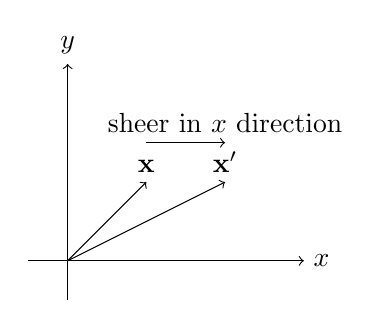
\begin{tikzpicture}
        \draw [->] (-0.5, 0) -- (3, 0) node [right] {$x$};
        \draw [->] (0, -0.5) -- (0, 2.5) node [above] {$y$};
        \draw [->] (0, 0) -- (1, 1) node [above] {$\mathbf{x}$};
        \draw [->] (0, 0) -- (2, 1) node [above] {$\mathbf{x}'$};
        \draw [->] (1, 1.5) -- (2, 1.5) node [align=center, above] {sheer in $x$ direction};
      \end{tikzpicture}
    \end{center}
    We have $(x, y, z)\mapsto (x + \lambda y, y, z)$. Then
    \[
      S =
      \begin{pmatrix}
        1 & \lambda & 0\\
        0 & 1 & 0\\
        0 & 0 & 1
      \end{pmatrix}
    \]
\end{enumerate}

\subsubsection{Matrix Algebra}
This part is mostly on a whole lot of definitions, saying what we can do with matrices and classifying them into different types.

\begin{defi}[Addition of matrices] Consider two linear maps $\alpha, \beta: \R^n\to \R^m$. The sum of $\alpha$ and $\beta$ is defined by
  \begin{align*}
    (\alpha + \beta)(\mathbf{x}) &= \alpha(\mathbf{x}) + \beta(\mathbf{x})\\
    \intertext{In terms of the matrix, we have}
    (A + B)_{ij}x_j &= A_{ij}x_j + B_{ij}x_j,\\
    \intertext{or}
    (A + B)_{ij} &= A_{ij}+B_{ij}.
  \end{align*}
\end{defi}

\begin{defi}[Scalar multiplication of matrices]
  Define $(\lambda\alpha)\mathbf{x} = \lambda[\alpha(\mathbf{x})]$. So $(\lambda A)_{ij} = \lambda A_{ij}$.
\end{defi}

\begin{defi}[Matrix multiplication]
  Consider maps $\alpha: \R^\ell \to \R^n$ and $\beta: \R^n\to \R^m$. The composition is $\beta\alpha:\R^\ell\to\R^m$. Take $\mathbf{x}\in \R^\ell\mapsto \mathbf{x}''\in \R^m$. Then $\mathbf{x}'' = (BA)\mathbf{x} = B\mathbf{x'}$, where $\mathbf{x}' = A\mathbf{x}$. Using suffix notation, we have $x_i'' = (B\mathbf{x}')_i = b_{ik}x_k' = B_{ik}A_{kj}x_j$. But $x_i'' = (BA)_{ij}x_j$. So
  \[
    (BA)_{ij} = B_{ik}A_{kj}.
  \]
  Generally, an $m\times n$ matrix multiplied by an $n\times \ell$ matrix gives an $m\times\ell$ matrix. $(BA)_{ij}$ is given by the $i$th row of $B$ dotted with the $j$th column of $A$.
\end{defi}
Note that the number of columns of $B$ has to be equal to the number of rows of $A$ for multiplication to be defined. If $\ell = m$ as well, then both $BA$ and $AB$ make sense, but $AB\not= BA$ in general. In fact, they don't even have to have the same dimensions.

Also, since function composition is associative, we get $A(BC) = (AB)C$.

\begin{defi}[Transpose of matrix]
  If $A$ is an $m\times n$ matrix, the \emph{transpose} $A^T$ is an $n\times m$ matrix defined by $(A^T)_{ij} = A_{ji}$.
\end{defi}

\begin{prop}\leavevmode
  \begin{enumerate}
    \item $(A^T)^T = A$.
    \item If $\mathbf{x}$ is a column vector$\begin{pmatrix}x_1\\x_2\\\vdots\\x_n\end{pmatrix}$, $\mathbf{x}^T$ is a row vector $(x_1\; x_2\cdots x_n)$.
    \item $(AB)^T = B^TA^T$ since $(AB)^T_{ij} = (AB)_{ji} = A_{jk}B_{ki} = B_{ki}A_{jk} $\\$= (B^T)_{ik}(A^T)_{kj} = (B^TA^T)_{ij}$.
  \end{enumerate}
\end{prop}

\begin{defi}[Hermitian conjugate]
  Define $A^{\dagger} = (A^T)^*$. Similarly, $(AB)^\dagger = B^\dagger A^\dagger$.
\end{defi}

\begin{defi}[Symmetric matrix]
  A matrix is \emph{symmetric} if $A^T = A$.
\end{defi}

\begin{defi}[Hermitian matrix]
  A matrix is \emph{Hermitian} if $A^\dagger = A$. (The diagonal of a Hermitian matrix must be real).
\end{defi}

\begin{defi}[Anti/skew symmetric matrix]
  A matrix is \emph{anti-symmetric} or \emph{skew symmetric} if $A^T = -A$. The diagonals are all zero.
\end{defi}

\begin{defi}[Skew-Hermitian matrix]
  A matrix is \emph{skew-Hermitian} if $A^\dagger = -A$. The diagonals are pure imaginary.
\end{defi}

\begin{defi}[Trace of matrix]
  The \emph{trace} of an $n\times n$ matrix $A$ is the sum of the diagonal. $\tr(A) = A_{ii}$.
\end{defi}

\begin{eg}
  Consider the reflection matrix $R_{ij} = \delta_{ij} - 2\hat n_i \hat n_j$. We have $\tr(A) = R_{ii} = 3 - 2\hat{n}\cdot \hat{n} = 3 - 2 = 1$.
\end{eg}

\begin{prop}
  $\tr(BC) = \tr(CB)$
\end{prop}

\begin{proof}
  $\tr(BC) = B_{ik}C_{ki} = C_{ki}B_{ik} = (CB)_{kk} = \tr(CB)$
\end{proof}

\begin{defi}[Identity matrix]
  $I = \delta_{ij}$.
\end{defi}
\subsubsection{Decomposition of an \texorpdfstring{$n\times n$}{n x n} matrix}
Any $n\times n$ matrix $B$ can be split as a sum of symmetric and antisymmetric parts. Write
\[
  B_{ij} = \underbrace{\frac{1}{2}(B_{ij} + B_{ji})}_{S_{ij}} + \underbrace{\frac{1}{2}(B_{ij} - B_{ji})}_{A_{ij}}.
\]
We have $S_{ij} = S_{ji}$, so $S$ is symmetric, while $A_{ji} = -A_{ij}$, and $A$ is antisymmetric. So $B = S + A$.

Furthermore , we can decompose $S$ into an isotropic part (a scalar multiple of the identity) plus a trace-less part (i.e.\ sum of diagonal $= 0$). Write
\[
  S_{ij} = \underbrace{\frac{1}{n}\tr (S)\delta_{ij}}_{\text{isotropic part}} + \underbrace{(S_{ij} - \frac{1}{n}\tr(S)\delta_{ij})}_{T_{ij}}.
\]
We have $\tr(T) = T_{ii} = S_{ii} - \frac{1}{n}\tr(S)\delta_{ii} = \tr(S) - \frac{1}{n}\tr(S)(n) = 0$.

Putting all these together,
\[
  B = \frac{1}{n}\tr(B)I + \left\{\frac{1}{2}(B + B^T) - \frac{1}{n}\tr(B)I\right\} + \frac{1}{2}(B - B^T).
\]
In three dimensions, we can write the antisymmetric part $A$ in terms of a single vector: we have
\[
  A = \begin{pmatrix}
    0 & a & -b\\
    -a & 0 & c\\
    b & -c & 0
  \end{pmatrix}
\]
and we can consider
\[
  \varepsilon_{ijk}\omega_k =
  \begin{pmatrix}
    0 & \omega_3 & -\omega_2\\
    -\omega_3 & 0 & \omega_1\\
    \omega_2 & -\omega_1 & 0
  \end{pmatrix}
\]
So if we have $\mathbf{\omega} = (c, b, a)$, then $A_{ij} = \varepsilon_{ijk}\omega_k$.

This decomposition can be useful in certain physical applications. For example, if the matrix represents the stress of a system, different parts of the decomposition will correspond to different types of stresses.

\subsubsection{Matrix inverse}

\begin{defi}[Inverse of matrix]
  Consider an $m\times n$ matrix $A$ and $n\times m$ matrices $B$ and $C$. If $BA = I$, then we say $B$ is the \emph{left inverse} of $A$. If $AC = I$, then we say $C$ is the \emph{right inverse} of $A$. If $A$ is square ($n\times n$), then $B = B(AC) = (BA)C = C$, i.e.\ the left and right inverses coincide. Both are denoted by $A^{-1}$, the \emph{inverse} of $A$. Therefore we have
  \[
    AA^{-1} = A^{-1}A = I.
  \]
\end{defi}
Note that not all square matrices have inverses. For example, the zero matrix clearly has no inverse.

\begin{defi}[Invertible matrix]
  If $A$ has an inverse, then $A$ is \emph{invertible}.
\end{defi}

\begin{prop}
  $(AB)^{-1} = B^{-1}A^{-1}$
\end{prop}

\begin{proof}
  $(B^{-1}A^{-1})(AB) = B^{-1}(A^{-1}A)B = B^{-1}B = I$.
\end{proof}

\begin{defi}[Orthogonal and unitary matrices]
  A real $n\times n$ matrix is \emph{orthogonal} if $A^TA = AA^T = I$, i.e.\ $A^T = A^{-1}$. A complex $n\times n$ matrix is \emph{unitary} if $U^\dagger U = UU^\dagger = I$, i.e.\ $U^\dagger = U^{-1}$.
\end{defi}
Note that an orthogonal matrix $A$ satisfies $A_{ik}(A^T_{kj}) = \delta_{ij}$, i.e.\ $A_{ik}A_{jk} = \delta_{ij}$. We can see this as saying ``the scalar product of two distinct rows is 0, and the scalar product of a row with itself is 1''. Alternatively, the rows (and columns --- by considering $A^T$) of an orthogonal matrix form an orthonormal set.

Similarly, for a unitary matrix, $U_{ik}U_{kj}^\dagger = \delta_{ij}$, i.e.\ $u_{ik}u_{jk}^* = u_{ik}^*u_{jk} =\delta_{ij}$. i.e.\ the rows are orthonormal, using the definition of complex scalar product.

\begin{eg}\leavevmode
  \begin{enumerate}
    \item The reflection in a plane is an orthogonal matrix. Since $R_{ij} = \delta_{ij} - 2n_in_j$, We have
      \begin{align*}
        R_{ik}R_{jk} &= (\delta_{ik} - 2n_in_k)(\delta_{jk} - 2n_jn_k)\\
        &= \delta_{ik}\delta_{jk} - 2\delta_{jk}n_in_k - 2\delta_{ik}n_jn_k + 2n_in_kn_jn_k\\
        &= \delta_{ij} - 2n_in_j - 2n_jn_i + 4n_in_j(n_kn_k)\\
        &= \delta_{ij}
      \end{align*}
    \item The rotation is an orthogonal matrix. We could multiply out using suffix notation, but it would be cumbersome to do so. Alternatively, denote rotation matrix by $\theta$ about $\mathbf{\hat n}$ as $R(\theta, \mathbf{\hat n})$. Clearly, $R(\theta, \mathbf{\hat n})^{-1} = R(-\theta, \mathbf{\hat n})$. We have
      \begin{align*}
        R_{ij}(-\theta, \mathbf{\hat n}) &= (\cos\theta)\delta_{ij} + n_in_j(1 - \cos\theta) + \varepsilon_{ijk}n_k\sin\theta\\
        &= (\cos\theta)\delta_{ji} + n_jn_i(1 - \cos\theta) - \varepsilon_{jik}n_k\sin\theta\\
        &= R_{ji}(\theta, \mathbf{\hat n})
      \end{align*}
      In other words, $R(-\theta, \mathbf{\hat n}) = R(\theta, \mathbf{\hat n})^T$. So $R(\theta, \mathbf{\hat n})^{-1} = R(\theta, \mathbf{\hat n})^T$.
  \end{enumerate}
\end{eg}

\subsection{Determinants}
Consider a linear map $\alpha: \R^3\to \R^3$. The standard basis $\mathbf{e}_1, \mathbf{e}_2, \mathbf{e}_3$ is mapped to $\mathbf{e}_1', \mathbf{e}_2', \mathbf{e}_3'$ with $\mathbf{e}_i' = A\mathbf{e}_i$. Thus the unit cube formed by $\mathbf{e}_1, \mathbf{e}_2, \mathbf{e}_3$ is mapped to the parallelepiped with volume
\begin{align*}
  [\mathbf{e}_1', \mathbf{e}_2', \mathbf{e}_3'] &= \varepsilon_{ijk}(e_1')_i (e_2')_j (e_3')_k\\
  &= \varepsilon_{ijk} A_{i\ell} \underbrace{(e_1)_\ell}_{\delta_{1\ell}} A_{jm}\underbrace{(e_2)_m}_{\delta_{2m}} A_{kn}\underbrace{(e_3)_n}_{\delta_{3n}}\\
  &= \varepsilon_{ijk} A_{i1}A_{j2}A_{k3}
\end{align*}
We call this the determinant and write as
\[
  \det(A) = \begin{vmatrix} A_{11} & A_{12} & A_{13}\\A_{21} & A_{22} & A_{23} \\ A_{31} & A_{32} & A_{33}\end{vmatrix}
\]

\subsubsection{Permutations}
To define the determinant for square matrices of arbitrary size, we first have to consider \emph{permutations}.

\begin{defi}[Permutation]
  A \emph{permutation} of a set $S$ is a bijection $\varepsilon: S\to S$.
\end{defi}

\begin{notation}
  Consider the set $S_n$ of all permutations of $1, 2, 3, \cdots , n$. $S_n$ contains $n!$ elements. Consider $\rho\in S_n$ with $i \mapsto \rho(i)$. We write
  \[
    \rho = \begin{pmatrix} 1 & 2 & \cdots & n\\ \rho(1) & \rho (2) &\cdots & \rho (n)\end{pmatrix}.
  \]
\end{notation}

\begin{defi}[Fixed point]
  A \emph{fixed point} of $\rho$ is a $k$ such that $\rho(k) = k$. e.g.\ in $\begin{pmatrix} 1 & 2 & 3 & 4\\4 & 1 & 3 & 2\end{pmatrix}$, $3$ is the fixed point. By convention, we can omit the fixed point and write as $\begin{pmatrix} 1 & 2 & 4\\ 4 & 1 & 2\end{pmatrix}$.
\end{defi}

\begin{defi}[Disjoint permutation]
  Two permutations are \emph{disjoint} if numbers moved by one are fixed by the other, and vice versa. e.g.\ $\begin{pmatrix} 1 & 2 & 4 & 5 & 6\\ 5 & 6 & 1 & 4 & 2\end{pmatrix} = \begin{pmatrix}2 & 6\\ 6& 2\end{pmatrix}\begin{pmatrix}1 & 4 & 5\\5 & 1 & 4\end{pmatrix}$, and the two cycles on the right hand side are disjoint. Disjoint permutations commute, but in general non-disjoint permutations do not.
\end{defi}

\begin{defi}[Transposition and $k$-cycle]
  $\begin{pmatrix} 2 & 6 \\ 6 & 2\end{pmatrix}$ is a \emph{2-cycle} or a \emph{transposition}, and we can simply write $(2\; 6)$. $\begin{pmatrix}1 & 4 & 5\\5 & 1 & 4\end{pmatrix}$ is a 3-cycle, and we can simply write $(1\; 5\; 4)$. (1 is mapped to 5; 5 is mapped to 4; 4 is mapped to 1)
\end{defi}

\begin{prop}
  Any $q$-cycle can be written as a product of 2-cycles.
\end{prop}

\begin{proof}
  $(1\; 2\; 3\; \cdots \; n) = (1\; 2)(2\; 3)(3\; 4)\cdots (n-1\; n)$.
\end{proof}

\begin{defi}[Sign of permutation]
  The \emph{sign} of a permutation $\varepsilon(\rho)$ is $(-1)^r$, where $r$ is the number of 2-cycles when $\rho$ is written as a product of 2-cycles. If $\varepsilon(\rho) = +1$, it is an even permutation. Otherwise, it is an odd permutation. Note that $\varepsilon(\rho\sigma) = \varepsilon(\rho)\varepsilon(\sigma)$ and $\varepsilon(\rho^{-1}) = \varepsilon(\rho)$.
\end{defi}
The proof that this is well-defined can be found in IA Groups.

\begin{defi}[Levi-Civita symbol]
  The \emph{Levi-Civita} symbol is defined by
  \[
    \varepsilon_{j_1j_2\cdots j_n} = \begin{cases}+1 & \text{ if } j_1j_2j_3\cdots j_n\text{ is an even permutation of }1, 2, \cdots n\\
      -1 & \text{ if it is an odd permutation}\\
      0 & \text{ if any 2 of them are equal}
    \end{cases}
  \]
  Clearly, $\varepsilon_{\rho(1)\rho(2)\cdots \rho(n)} = \varepsilon(\rho)$.
\end{defi}

\begin{defi}[Determinant]
  The \emph{determinant} of an $n\times n$ matrix $A$ is defined as:
  \[
    \det (A) = \sum_{\sigma\in S_n} \varepsilon(\sigma) A_{\sigma(1)1}A_{\sigma(2)2}\cdots A_{\sigma(n)n},
  \]
  or equivalently,
  \[
    \det(A) = \varepsilon_{j_1j_2\cdots j_n}A_{j_11}A_{j_22}\cdots A_{j_nn}.
  \]
\end{defi}

\begin{prop}
  \[
    \begin{vmatrix}
      a & b\\
      c & d
    \end{vmatrix} = ad - bc
  \]
\end{prop}

\subsubsection{Properties of determinants}
\begin{prop}
  $\det (A) = \det (A^T)$.
\end{prop}

\begin{proof}
  Take a single term $A_{\sigma(1)1}A_{\sigma(2)2}\cdots A_{\sigma(n)n}$ and let $\rho$ be another permutation in $S_n$. We have
  \[
    A_{\sigma(1)1}A_{\sigma(2)2}\cdots A_{\sigma(n)n} = A_{\sigma(\rho(1))\rho(1)}A_{\sigma(\rho(2))\rho(2)}\cdots A_{\sigma(\rho(n))\rho(n)}
  \]
  since the right hand side is just re-ordering the order of multiplication. Choose $\rho = \sigma^{-1}$ and note that $\varepsilon(\sigma) = \varepsilon(\rho)$. Then
  \[
    \det(A) = \sum_{\rho\in S_n} \varepsilon(\rho) A_{1\sigma(1)}A_{2\sigma(2)}\cdots A_{n\sigma(n)} = \det (A^T). \qedhere
  \]
\end{proof}

\begin{prop}
  If matrix $B$ is formed by multiplying every element in a single row of $A$ by a scalar $\lambda$, then $\det (B) = \lambda \det (A)$. Consequently, $\det (\lambda A) = \lambda^n \det(A)$.
\end{prop}

\begin{proof}
  Each term in the sum is multiplied by $\lambda$, so the whole sum is multiplied by $\lambda^n$.
\end{proof}

\begin{prop}
  If 2 rows (or 2 columns) of $A$ are identical, the determinant is $0$.
\end{prop}

\begin{proof}
  wlog, suppose columns 1 and 2 are the same. Then
  \[
    \det (A) = \sum_{\sigma\in S_n} \varepsilon(\sigma) A_{\sigma(1)1}A_{\sigma(2)2}\cdots A_{\sigma(n)n}.
  \]
  Now write an arbitrary $\sigma$ in the form $\sigma = \rho(1\; 2)$. Then $\varepsilon(\sigma) = \varepsilon(\rho)\varepsilon((1\; 2)) = -\varepsilon(\rho)$. So
  \[
    \det (A) = \sum_{\rho\in S_n} -\varepsilon(\rho) A_{\rho(2)1}A_{\rho(1)2}A_{\rho(3)3}\cdots A_{\rho(n)n}.
  \]
  But columns 1 and 2 are identical, so $A_{\rho(2)1} = A_{\rho(2)2}$ and $A_{\rho(1)2} = A_{\rho(1)1}$. So $\det (A) = -\det (A)$ and $\det(A) = 0$.
\end{proof}

\begin{prop}
  If 2 rows or 2 columns of a matrix are linearly dependent, then the determinant is zero.
\end{prop}

\begin{proof}
  Suppose in $A$, $($column $r) + \lambda($column $s) = 0$. Define
  \[
    B_{ij} =
    \begin{cases}
      A_{ij} & j\not= r\\
      A_{ij} + \lambda A_{is} & j = r
    \end{cases}.
  \]
  Then $\det (B) = \det(A) + \lambda \det($matrix with column $r =$ column $s) = \det(A)$. Then we can see that the $r$th column of $B$ is all zeroes. So each term in the sum contains one zero and $\det (A) = \det (B) = 0$.
\end{proof}
Even if we don't have linearly dependent rows or columns, we can still run the exact same proof as above, and still get that $\det (B) = \det (A)$. Linear dependence is only required to show that $\det (B) = 0$. So in general, we can add a linear multiple of a column (or row) onto another column (or row) without changing the determinant.

\begin{prop}
  Given a matrix $A$, if $B$ is a matrix obtained by adding a multiple of a column (or row) of $A$ to another column (or row) of $A$, then $\det A = \det B$.
\end{prop}

\begin{cor}
  Swapping two rows or columns of a matrix negates the determinant.
\end{cor}

\begin{proof}
  We do the column case only. Let $A = (\mathbf{a}_1 \cdots \mathbf{a}_i \cdots \mathbf{a}_j \cdots \mathbf{a}_n)$. Then
  \begin{align*}
    \det (\mathbf{a}_1 \cdots \mathbf{a}_i \cdots \mathbf{a}_j \cdots \mathbf{a}_n)&=\det(\mathbf{a}_1 \cdots \mathbf{a}_i + \mathbf{a}_j \cdots \mathbf{a}_j \cdots \mathbf{a}_n)\\
    &=\det (\mathbf{a}_1 \cdots \mathbf{a}_i + \mathbf{a}_j \cdots \mathbf{a}_j - (\mathbf{a}_i + \mathbf{a}_j) \cdots \mathbf{a}_n)\\
    &=\det (\mathbf{a}_1 \cdots \mathbf{a}_i + \mathbf{a}_j \cdots -\mathbf{a}_i \cdots \mathbf{a}_n)\\
    &=\det (\mathbf{a}_1 \cdots \mathbf{a}_j \cdots -\mathbf{a}_i \cdots \mathbf{a}_n)\\
    &=-\det (\mathbf{a}_1 \cdots \mathbf{a}_j \cdots \mathbf{a}_i \cdots \mathbf{a}_n)
  \end{align*}
  Alternatively, we can prove this from the definition directly, using the fact that the sign of a transposition is $-1$ (and that the sign is multiplicative).
\end{proof}

\begin{prop}
  $\det(AB) = \det(A)\det(B)$.
\end{prop}

\begin{proof}
  First note that $\sum_\sigma \varepsilon(\sigma)A_{\sigma(1)\rho(1)}A_{\sigma(2)\rho(2)} = \varepsilon(\rho)\det (A)$, i.e.\ swapping columns (or rows) an even/odd number of times gives a factor $\pm 1$ respectively. We can prove this by writing $\sigma = \mu \rho$.

  Now
  \begin{align*}
    \det AB &= \sum_\sigma \varepsilon(\sigma)(AB)_{\sigma(1)1}(AB)_{\sigma(2)2}\cdots (AB)_{\sigma(n)n}\\
    &= \sum_\sigma \varepsilon(\sigma) \sum_{k_1,k_2,\cdots,k_n}^{n} A_{\sigma(1)k_1}B_{k_11}\cdots A_{\sigma(n)k_n}B_{k_nn}\\
    &= \sum_{k_1,\cdots,k_n}B_{k_11}\cdots B_{k_nn}\underbrace{\sum_\sigma \varepsilon(\sigma) A_{\sigma(1)k_1}A_{\sigma(2)k_2}\cdots A_{\sigma(n)k_n}}_{S}
    \intertext{Now consider the many different $S$'s. If in $S$, two of $k_1$ and $k_n$ are equal, then $S$ is a determinant of a matrix with two columns the same, i.e.\ $S = 0$. So we only have to consider the sum over distinct $k_i$s. Thus the $k_i$s are are a permutation of $1, \cdots n$, say $k_i =\rho (i)$. Then we can write}
    \det AB &= \sum_\rho B_{\rho(1)1}\cdots B_{\rho(n)n} \sum_\sigma \varepsilon(\sigma) A_{\sigma(1)\rho(1)} \cdots A_{\sigma(n)\rho(n)}\\
    &= \sum_\rho B_{\rho(1)1}\cdots B_{\rho(n)n} (\varepsilon(\rho)\det A)\\
    &= \det A\sum_\rho \varepsilon(\rho) B_{\rho(1)1}\cdots B_{\rho(n)n}\\
    &= \det A\det B \qedhere
  \end{align*}
\end{proof}

\begin{cor}
  If $A$ is orthogonal, $\det A = \pm 1$.
\end{cor}

\begin{proof}
  \begin{align*}
    AA^T &= I\\
    \det AA^T &= \det I\\
    \det A\det A^T &= 1\\
    (\det A)^2 &= 1\\
    \det A &= \pm 1 \qedhere
  \end{align*}
\end{proof}

\begin{cor}
  If $U$ is unitary, $|\det U| = 1$.
\end{cor}

\begin{proof}
  We have $\det U^\dagger = (\det U^T)^* = \det(U)^*$. Since $UU^\dagger = I$, we have $\det(U)\det(U)^* = 1$.
\end{proof}

\begin{prop}
  In $\R^3$, orthogonal matrices represent either a rotation ($\det = 1$) or a reflection ($\det = -1$).
\end{prop}
\subsubsection{Minors and Cofactors}
\begin{defi}[Minor and cofactor]
  For an $n\times n$ matrix $A$, define $A^{ij}$ to be the $(n - 1)\times (n - 1)$ matrix in which row $i$ and column $j$ of $A$ have been removed.

  The \emph{minor} of the $ij$th element of $A$ is $M_{ij} = \det A^{ij}$

  The \emph{cofactor} of the $ij$th element of $A$ is $\Delta_{ij} = (-1)^{i + j}M_{ij}$.
\end{defi}

\begin{notation}
  We use $\bar \;$ to denote a symbol which has been missed out of a natural sequence.
\end{notation}
\begin{eg}
  $1, 2, 3, 5 = 1, 2, 3, \bar 4, 5$.
\end{eg}

The significance of these definitions is that we can use them to provide a systematic way of evaluating determinants. We will also use them to find inverses of matrices.
\begin{thm}[Laplace expansion formula]
  For any particular fixed $i$,
  \[
    \det A = \sum_{j = 1}^{n} A_{ji}\Delta_{ji}.
  \]
\end{thm}
\begin{proof}
  \[
    \det A = \sum_{j_i = 1}^nA_{j_ii} \sum_{j_1, \cdots, \overline{j_i}, \cdots j_n}^n \varepsilon_{j_1j_2\cdots j_n} A_{j_11}A_{j_22}\cdots \overline{A_{j_ii}}\cdots A_{j_nn}
  \]
  Let $\sigma \in S_n$ be the permutation which moves $j_i$ to the $i$th position, and leave everything else in its natural order, i.e.\setcounter{MaxMatrixCols}{11}
  \[
    \sigma =
    \begin{pmatrix}
      1 &\cdots& i & i + 1 & i + 2 & \cdots &j_i - 1&j_i& j_i + 1 & \cdots & n\\
      1 & \cdots & j_i & i & i + 1 & \cdots & j_i - 2 & j_i - 1 & j_i + 1 & \cdots & n
    \end{pmatrix}
  \]
  if $j_i > i$, and similarly for other cases. To perform this permutation, $|i - j_i|$ transpositions are made. So $\varepsilon(\sigma) = (-1)^{i - j_i}$.

  Now consider the permutation $\rho\in S_n$
  \[
    \rho =
    \begin{pmatrix}
      1 & \cdots & \cdots & \bar {j_i} & \cdots & n\\
      j_1 & \cdots & \bar{j_i} & \cdots & \cdots & j_n\\
    \end{pmatrix}
  \]
  The composition $\rho\sigma$ reorders $(1, \cdots, n)$ to $(j_1, j_2,\cdots, j_n)$. So $\varepsilon(\rho\sigma) = \varepsilon_{j_1\cdots j_n} = \varepsilon(\rho)\varepsilon(\sigma) = (-1)^{i - j_i} \varepsilon_{j_1\cdots \bar j_i \cdots j_n}$. Hence the original equation becomes
  \begin{align*}
    \det A &= \sum_{j_i = 1}^n A_{j_i i} \sum_{j_1\cdots \bar j_i\cdots j_n}(-1)^{i - j_i} \varepsilon_{j_1\cdots \bar j_i \cdots j_n} A_{j_11}\cdots \overline{A_{j_ii}} \cdots A_{j_nn}\\
    &= \sum_{j_i = 1}^n A_{j_ii} (-1)^{i - j_i}M_{j_ii}\\
    &= \sum_{j_i = 1}^{n} A_{j_ii}\Delta_{j_ii}\\
    &= \sum_{j = 1}^{n} A_{ji}\Delta_{ji} \qedhere
  \end{align*} % Check!
\end{proof}

\begin{eg}
  $\det A = \begin{vmatrix}2 & 4 & 2\\ 3 & 2 & 1\\ 2 & 0 & 1\end{vmatrix}$. We can pick the first row and have
  \begin{align*}
    \det A&= 2\begin{vmatrix}2 & 1\\0 & 1 \end{vmatrix} - 4\begin{vmatrix} 3 & 1\\ 2 & 1\end{vmatrix} + 2\begin{vmatrix}3 & 2 \\ 2 & 0\end{vmatrix}\\
    &= 2(2 - 0) - 4(3 - 2) + 2(0 - 4)\\
    &= -8.
  \end{align*}
  Alternatively, we can pick the second column and have
  \begin{align*}
    \det A&= -4\begin{vmatrix}3 & 1\\2 & 1 \end{vmatrix} + 2\begin{vmatrix} 2 & 2\\ 2 & 1\end{vmatrix} - 0\begin{vmatrix}2 & 2 \\ 3 & 1\end{vmatrix}\\
    &= -4(3 - 2) + 2(2 - 4) - 0\\
    &= -8.
  \end{align*}
\end{eg}

In practical terms, we use a combination of properties of determinants with a sensible choice of $i$ to evaluate $\det(A)$.

\begin{eg}
  Consider $\begin{vmatrix}1 & a & a^2\\1 & b & b^2\\1 & c & c^2 \end{vmatrix}$. Row 1 - row 2 gives
  \[
    \begin{vmatrix}0 & a - b & a^2 - b^2\\1 & b & b^2\\1 & c & c^2 \end{vmatrix} = (a - b)\begin{vmatrix}0 & 1 & a + b\\1 & b & b^2\\1 & c & c^2 \end{vmatrix}.
  \]
  Do row 2 - row 3. We obtain
  \[
    (a - b)(b - c)\begin{vmatrix}0 & 1 & a + b\\0 & 1 & b + c\\1 & c & c^2 \end{vmatrix}.
  \]
  Row 1 - row 2 gives
  \[
    (a - b)(b - c)(a - c)\begin{vmatrix}0 & 0 & 1\\0 & 1 & b + c\\1 & c & c^2 \end{vmatrix} = (a - b)(b - c)(a - c).
  \]
\end{eg}

\section{Matrices and linear equations}
\subsection{Simple example, \texorpdfstring{$2\times 2$}{2 x 2}}
Consider the system of equations
\begin{align*}
  A_{11}x_1 + A_{12}x_2 &= d_1\tag{a}\\
  A_{21}x_1 + A_{22}x_2 &= d_2\tag{b}.
  \intertext{We can write this as}
  A\mathbf{x} &= \mathbf{d}.
\end{align*}
If we do (a)$\times A_{22} - $(b)$\times A_{12}$ and similarly the other way round, we obtain
\begin{align*}
  (A_{11}A_{22} - A_{12}A_{21})x_1 &= A_{22}d_1 - A_{12}d_2\\
  \underbrace{(A_{11}A_{22} - A_{12}A_{21})}_{\det A}x_2 &= A_{11}d_2 - A_{21}d_1
\end{align*}
Dividing by $\det A$ and writing in matrix form, we have
\[
  \begin{pmatrix}
    x_1\\
    x_2
  \end{pmatrix} = \frac{1}{\det A}
  \begin{pmatrix}
    A_{22} & - A_{12}\\
    -A_{21} & A_{11}
  \end{pmatrix}
  \begin{pmatrix}
    d_1\\
    d_2
  \end{pmatrix}
\]
On the other hand, given the equation $A\mathbf{x} = \mathbf{d}$, if $A^{-1}$ exists, then by multiplying both sides on the left by $A^{-1}$, we obtain $\mathbf{x} = A^{-1}\mathbf{d}$.

Hence, we have constructed $A^{-1}$ in the $2\times 2$ case, and shown that the condition for its existence is $\det A \not= 0$, with
\[
  A^{-1} =\frac{1}{\det A}\begin{pmatrix}A_{22} & - A_{12}\\-A_{21} & A_{11}\end{pmatrix}
\]

\subsection{Inverse of an \texorpdfstring{$n\times n$}{n x n} matrix}
For larger matrices, the formula for the inverse is similar, but slightly more complicated (and costly to evaluate). The key to finding the inverse is the following:
\begin{lemma}
  $\sum A_{ik}\Delta_{jk} = \delta_{ij}\det A$.
\end{lemma}

\begin{proof}
  If $i \not= j$, then consider an $n\times n$ matrix $B$, which is identical to $A$ except the $j$th row is replaced by the $i$th row of $A$. So $\Delta_{jk}$ of $B = \Delta_{jk}$ of $A$, since $\Delta_{jk}$ does not depend on the elements in row $j$. Since $B$ has a duplicate row, we know that
  \[
    0 = \det B = \sum_{k = 1}^n B_{jk}\Delta_{jk} = \sum_{k = 1}^n A_{ik}\Delta_{jk}.
  \]
  If $i = j$, then the expression is $\det A$ by the Laplace expansion formula.
\end{proof}

\begin{thm}
  If $\det A \not =0$, then $A^{-1}$ exists and is given by
  \[
    (A^{-1})_{ij} = \frac{\Delta_{ji}}{\det A}.
  \]
\end{thm}

\begin{proof}
  \[
    (A^{-1})_{ik}A_{kj} = \frac{\Delta_{ki}}{\det A} A_{kj} = \frac{\delta_{ij}\det A}{\det A} = \delta_{ij}.
  \]
  So $A^{-1}A = I$.
\end{proof}
The other direction is easy to prove. If $\det A = 0$, then it has no inverse, since for any matrix $B$, $\det AB = 0$, and hence $AB$ cannot be the identity.

\begin{eg}
  Consider the shear matrix $S_\lambda = \begin{pmatrix} 1 & \lambda & 0 \\ 0 & 1 & 0\\ 0 & 0 & 1\end{pmatrix}$. We have $\det{S_\lambda} = 1$. The cofactors are
  \begin{center}
    \begin{tabular}{ccc}
      $\Delta_{11} = 1$ & $\Delta_{12} = 0$ & $\Delta_{13} = 0$ \\
      $\Delta_{21} - \lambda$ & $\Delta_{22} = 1$ & $\Delta_{23} = 0$ \\
      $\Delta_{31} = 0$ & $\Delta_{32} = 0$ & $\Delta_{33} = 1$
    \end{tabular}
  \end{center}
  So $S_\lambda^{-1} = \begin{pmatrix} 1 & -\lambda & 0\\ 0 & 1 & 0\\ 0 & 0 & 1\end{pmatrix}$.
\end{eg}

How many arithmetic operations are involved in calculating the inverse of an $n\times n$ matrix? We just count multiplication operations since they are the most time-consuming. Suppose that calculating $\det A$ takes $f_n$ multiplications. This involves $n$ $(n - 1)\times (n - 1)$ determinants, and you need $n$ more multiplications to put them together. So $f_n = nf_{n -1} + n$. So $f_n = O(n!)$ (in fact $f_n \approx (1 + e)n!$).

To find the inverse, we need to calculate $n^2$ cofactors. Each is a $n -1$ determinant, and each takes $O((n - 1)!)$. So the time complexity is $O(n^2 (n - 1)!) = O(n\cdot n!)$.

This is incredibly slow. Hence while it is theoretically possible to solve systems of linear equations by inverting a matrix, sane people do not do so in general. Instead, we develop certain better methods to solve the equations. In fact, the ``usual'' method people use to solve equations by hand only has complexity $O(n^3)$, which is a much better complexity.

\subsection{Homogeneous and inhomogeneous equations}
Consider $A\mathbf{x} = \mathbf{b}$ where $A$ is an $n\times n$ matrix, $\mathbf{x}$ and $\mathbf{b}$ are $n\times 1$ column vectors.
\begin{defi}[Homogeneous equation]
  If $\mathbf{b} = \mathbf{0}$, then the system is \emph{homogeneous}. Otherwise, it's \emph{inhomogeneous}.
\end{defi}

Suppose $\det A\not= 0$. Then there is a unique solution $\mathbf{x} = A^{-1}\mathbf{b}$ ($\mathbf{x} = \mathbf{0}$ for homogeneous).

How can we understand this result? Recall that $\det A\not= 0$ means that the columns of $A$ are linearly independent. The columns are the images of the standard basis, $\mathbf{e}_i' = A\mathbf{e_i}$. So $\det A\not = 0$ means that $\mathbf{e}_i'$ are linearly independent and form a basis of $\R^n$. Therefore the image is the whole of $\R^n$. This automatically ensures that $\mathbf{b}$ is in the image, i.e.\ there is a solution.

To show that there is exactly one solution, suppose $\mathbf{x}$ and $\mathbf{x}'$ are both solutions. Then $A\mathbf{x} = A\mathbf{x}' = \mathbf{b}$. So $A(\mathbf{x} - \mathbf{x}') = \mathbf{0}$. So $\mathbf{x} - \mathbf{x}'$ is in the kernel of $A$. But since the rank of $A$ is $n$, by the rank-nullity theorem, the nullity is $0$. So the kernel is trivial. So $\mathbf{x} - \mathbf{x}' = \mathbf{0}$, i.e.\ $\mathbf{x} = \mathbf{x}'$.

\subsubsection{Gaussian elimination}
Consider a general solution
\begin{align*}
  A_{11}x_1 + A_{12}x_2 + \cdots + A_{1n}x_n &= d_1\\
  A_{21}x_1 + A_{22}x_2 + \cdots + A_{2n}x_n &= d_2\\
  \vdots&\\
  A_{m1}x_1 + A_{m2}x_2 + \cdots + A_{mn}x_n &= d_m
\end{align*}
So we have $m$ equations and $n$ unknowns.

Assume $A_{11}\not=0$ (if not, we can re-order the equations). We can use the first equation to eliminate $x_1$ from the remaining $(m - 1)$ equations. Then use the second equation to eliminate $x_2$ from the remaining $(m - 2)$ equations (if anything goes wrong, just re-order until things work). Repeat.

We are left with
\begin{align*}
  A_{11}x_1 + A_{12}x_2 + A_{13}x_3 + \cdots + A_{1n}x_n &= d_1\\
  A_{22}^{(2)}x_2 + A_{23}^{(2)}x_3 + \cdots + A_{2n}^{(2)}x_n &= d_2\\
  \vdots&\\
  A_{rr}^{(r)}x_r + \cdots + A_{rn}^{(r)}x_n &= d_r\\
  0 &= d_{r + 1}^{(r)}\\
  \vdots&\\
  0 &= d_{m}^{(r)}
\end{align*}
Here $A_{ii}^{(i)} \not=0$ (which we can achieve by re-ordering), and the superfix $(i)$ refers to the ``version number'' of the coefficient, e.g.\ $A_{22}^{(2)}$ is the second version of the coefficient of $x_2$ in the second row.

Let's consider the different possibilities:
\begin{enumerate}
  \item $r < m$ and at least one of $d^{(r)}_{r + 1}, \cdots d_m^{(r)} \not= 0$. Then a contradiction is reached. The system is inconsistent and has no solution. We say it is \emph{overdetermined}.
    \begin{eg}
      Consider the system
      \begin{align*}
        3x_1 + 2x_2 + x_3 &= 3\\
        6x_1 + 3x_2 + 3x_3 &= 0\\
        6x_1 + 2x_2 + 4x_3 &= 6
        \intertext{This becomes }
        3x_1 + 2x_2 + x_3 &= 3\\
        0 - x_2 + x_3 &= -6\\
        0 - 2x_2 + 2x_3 &= 0
        \intertext{And then}
        3x_1 + 2x_2 + x_3 &= 3\\
        0 - x_2 + x_3 &= -6\\
        0 &= 12
      \end{align*}
      We have $d_3^{(3)} = 12 = 0$ and there is no solution.
    \end{eg}
  \item If $r = n\leq m$, and all $d_{r + i}^{(r)} = 0$. Then from the $n$th equation, there is a unique solution for $x_n = d_{n}^{(n)}/A_{nn}^{(n)}$, and hence for all $x_i$ by back substitution. This system is \emph{determined}.
    \begin{eg}
      \begin{align*}
        2x_1 + 5x_2 &= 2\\
        4x_1 + 3x_2 &= 11\\
        \intertext{This becomes}
        2x_1 + 5x_2 &= 2\\
        -7x_2 &= 7
      \end{align*}
      So $x_2 = -1$ and thus $x_1 = 7/2$.
    \end{eg}
  \item If $r < n$ and $d_{r + i}^{(r)} = 0$, then $x_{r + 1}, \cdots x_n$ can be freely chosen, and there are infinitely many solutions. System is \emph{under-determined}. e.g.
    \begin{align*}
      x_1 + x_2 &= 1\\
      2x_1 + 2x_2 &= 2
      \intertext{Which gives}
      x_1 + x_2 &= 1\\
      0 &= 0
    \end{align*}
    So $x_1 = 1 - x_2$ is a solution for any $x_2$.
\end{enumerate}
In the $n = m$ case, there are $O(n^3)$ operations involved, which is much less than inverting the matrix. So this is an efficient way of solving equations.

This is also be related to the determinant. Consider the case where $m = n$ and $A$ is square. Since row operations do not change the determinant and swapping rows give a factor of $(-1)$. So
\[
  \det A = (-1)^k
  \begin{vmatrix}
    A_{11} &A_{12}&\cdots& \cdots& \cdots & A_{1n}\\
    0 & A_{22}^{(2)} &\cdots& \cdots & \cdots & A_{2n}^{(n)} \\
    \vdots & \vdots &\ddots & \vdots & \vdots & \vdots\\
    0 & 0 & \cdots & A_{rr}^{(r)} & \cdots & A_{rn}^{(n)}\\
    0 & 0 & \cdots & 0 & 0 & \cdots\\
    \vdots & \vdots & \vdots & \vdots & \vdots & \vdots
  \end{vmatrix}
\]
This determinant is an \emph{upper triangular} one (all elements below diagonal are $0$) and the determinant is the product of its diagonal elements.

Hence if $r < n$ (and $d_i^{(r)} = 0$ for $i > r$), then we have case (ii) and the $\det A = 0$. If $r = n$, then $\det A = (-1)^k A_{11}A_{22}^{(2)}\cdots A_{nn}^{(n)} \not= 0$.

\subsection{Matrix rank}
Consider a linear map $\alpha: \R^n\to \R^m$. Recall the rank $r(\alpha)$ is the dimension of the image. Suppose that the matrix $A$ is associated with the linear map. We also call $r(A)$ the \emph{rank} of $A$.

Recall that if the standard basis is $\mathbf{e}_1,\cdots \mathbf{e}_n$, then $A\mathbf{e}_1, \cdots, A\mathbf{e}_n$ span the image (but not necessarily linearly independent).

Further, $A\mathbf{e}_1, \cdots, A\mathbf{e}_n$ are the columns of the matrix $A$. Hence $r(A)$ is the number of linearly independent columns.

\begin{defi}[Column and row rank of linear map]
  The \emph{column rank} of a matrix is the maximum number of linearly independent columns.

  The \emph{row rank} of a matrix is the maximum number of linearly independent rows.
\end{defi}

\begin{thm}
  The column rank and row rank are equal for any $m\times n$ matrix.
\end{thm}

\begin{proof}
  Let $r$ be the row rank of $A$. Write the biggest set of linearly independent rows as $\mathbf{v}_1^T, \mathbf{v}_2^T, \cdots \mathbf{v}_r^T$ or in component form $\mathbf{v}_k^T = (v_{k1}, v_{k2}, \cdots, v_{kn})$ for $k = 1, 2, \cdots, r$.

  Now denote the $i$th row of $A$ as $\mathbf{r}_i^T = (A_{i1}, A_{i2}, \cdots A_{in})$.

  Note that every row of $A$ can be written as a linear combination of the $\mathbf{v}$'s. (If $\mathbf{r_i}$ cannot be written as a linear combination of the $\mathbf{v}$'s, then it is independent of the $\mathbf{v}$'s and $\mathbf{v}$ is not the maximum collection of linearly independent rows) Write
  \[
    \mathbf{r}_i^T = \sum_{k = 1}^r C_{ik}\mathbf{v}_{k}^T.
  \]
  For some coefficients $C_{ik}$ with $1 \leq i\leq m$ and $1 \leq k \leq r$.

  Now the elements of $A$ are
  \[
    A_{ij} = (\mathbf{r}_i)^T_j = \sum_{k = 1}^r C_{ik}(\mathbf{v}_k)_j,
  \]
  or
  \[
    \begin{pmatrix}
      A_{1j}\\
      A_{2j}\\
      \vdots\\
      A_{mj}
    \end{pmatrix} = \sum_{k = 1}^r {\mathbf{v}_k}_j
    \begin{pmatrix}
      C_{1k}\\
      C_{2k}\\\
      \vdots\\
      C_{mk}
    \end{pmatrix}
  \]
  So every column of $A$ can be written as a linear combination of the $r$ column vectors $\mathbf{c}_k$. Then the column rank of $A \leq r$, the row rank of $A$.

  Apply the same argument to $A^T$ to see that the row rank is $\leq$ the column rank.
\end{proof}

\subsection{Homogeneous problem \texorpdfstring{$A\mathbf{x} = \mathbf{0}$}{Ax = 0}}
We restrict our attention to the square case, i.e.\ number of unknowns = number of equations. Here $A$ is an $n\times n$ matrix. We want to solve $A\mathbf{x} = \mathbf{0}$.

First of all, if $\det A\not=0$, then $A^{-1}$ exists and $\mathbf{x}^{-1} = A^{-1}\mathbf{0} = \mathbf{0}$, which is the unique solution. Hence if $A\mathbf{x} = \mathbf{0}$ with $\mathbf{x} \not= \mathbf{0}$, then $\det A = 0$.

\subsubsection{Geometrical interpretation}
We consider a $3\times 3$ matrix
\[
  A = \begin{pmatrix} \mathbf{r}_1^T\\\mathbf{r}_2^T\\\mathbf{r}_3^T\end{pmatrix}
\]
$A\mathbf{x} = \mathbf{0}$ means that $\mathbf{r}_i\cdot \mathbf{x} = 0$ for all $i$. Each equation $\mathbf{r}_i\cdot \mathbf{x} = 0$ represents a plane through the origin. So the solution is the intersection of the three planes.

There are three possibilities:
\begin{enumerate}
  \item If $\det A =[\mathbf{r}_1, \mathbf{r}_2, \mathbf{r}_3] \not= 0$, span$\{\mathbf{r}_1, \mathbf{r}_2, \mathbf{r}_3\} = \R^3$ and thus $r(A) = 3$. By the rank-nullity theorem, $n(A) = 0$ and the kernel is $\{\mathbf{0}\}$. So $\mathbf{x} = \mathbf{0}$ is the unique solution.
  \item If $\det A = 0$, then $\dim(\spn\{\mathbf{r}_1, \mathbf{r}_2, \mathbf{r}_3\}) = 1$ or $2$.
    \begin{enumerate}
      \item If rank $= 2$, wlog assume $\mathbf{r}_1, \mathbf{r}_2$ are linearly independent. So $\mathbf{x}$ lies on the intersection of two planes $\mathbf{x}\cdot \mathbf{r}_1 = 0$ and $\mathbf{x}\cdot \mathbf{r}_2 = 0$, which is the line $\{\mathbf{x}\in \R^3: \mathbf{x} = \lambda \mathbf{r}_1\times \mathbf{r}_2\}$ (Since $\mathbf{x}$ lies on the intersection of the two planes, it has to be normal to the normals of both planes). All such points on this line also satisfy $\mathbf{x}\cdot\mathbf{r}_3 = 0$ since $\mathbf{r}_3$ is a linear combination of $\mathbf{r}_1$ and $\mathbf{r}_2$. The kernel is a line, $n(A) = 1$.
      \item If rank = 1, then $\mathbf{r}_1, \mathbf{r}_2, \mathbf{r}_3$ are parallel. So $\mathbf{x}\cdot \mathbf{r}_1 = 0 \Rightarrow \mathbf{x}\cdot \mathbf{r}_2 = \mathbf{x}\cdot \mathbf{r}_3 = 0$. So all $\mathbf{x}$ that satisfy $\mathbf{x}\cdot \mathbf{r}_1 = 0$ are in the kernel, and the kernel now is a plane. $n(A) = 2$.
    \end{enumerate}
\end{enumerate}
(We also have the trivial case where $r(A) = 0$, we have the zero mapping and the kernel is $\R^3$)

\subsubsection{Linear mapping view of \texorpdfstring{$A\mathbf{x} = \mathbf{0}$}{Ax = 0}}
In the general case, consider a linear map $\alpha: \R^n \to \R^n$ $\mathbf{x} \mapsto \mathbf{x}' = A\mathbf{x}$. The kernel $k(A) = \{\mathbf{x}\in \R^n: A\mathbf{x} = \mathbf{0}\}$ has dimension $n(A)$.

\begin{enumerate}
  \item If $n(A) = 0$, then $A(\mathbf{e}_1), A(\mathbf{e}_2), \cdots, A(\mathbf{e}_n)$ is a linearly independent set, and $r(A) = n$.
  \item If $n(A) > 0$, then the image is not the whole of $\R^n$. Let $\{\mathbf{u}_i\}, i = 1, \cdots, n(A)$ be a basis of the kernel, i.e.\ so given any solution to $A\mathbf{x} = \mathbf{0}$, $\displaystyle \mathbf{x} = \sum_{i = 1}^{n(A)} \lambda_i \mathbf{u}_i$ for some $\lambda_i$. Extend $\{\mathbf{u}_i\}$ to be a basis of $\R^n$ by introducing extra vectors $\mathbf{u}_{i}$ for $i = n(A) + 1, \cdots, n$. The vectors $A(\mathbf{u}_i)$ for $i = n(A) + 1, \cdots, n$ form a basis of the image.
\end{enumerate}

\subsection{General solution of \texorpdfstring{$A\mathbf{x} = \mathbf{d}$}{Ax = d}}
Finally consider the general equation $A\mathbf{x} = \mathbf{d}$, where $A$ is an $n\times n$ matrix and $\mathbf{x}, \mathbf{d}$ are $n \times 1$ column vectors. We can separate into two main cases.

\begin{enumerate}
  \item $\det(A) \not= 0$. So $A^{-1}$ exists and $n(A) = 0$, $r(A) = n$. Then for any $\mathbf{d}\in \R^n$, a unique solution must exists and it is $\mathbf{x} = A^{-1}\mathbf{d}$.
  \item $\det(A) = 0$. Then $A^{-1}$ does not exist, and $n(A) > 0$, $r(A) < n$. So the image of $A$ is not the whole of $\R^n$.
    \begin{enumerate}
      \item If $\mathbf{d}\not\in \im A$, then there is no solution (by definition of the image)
      \item If $\mathbf{d}\in \im A$, then by definition there exists at least one $\mathbf{x}$ such that $A\mathbf{x} = \mathbf{d}$. The general solution of $A\mathbf{x} = \mathbf{d}$ can be written as $\mathbf{x} = \mathbf{x}_0 + \mathbf{y}$, where $\mathbf{x}_0$ is a particular solution (i.e.\ $A\mathbf{x}_0 = \mathbf{d}$), and $\mathbf{y}$ is any vector in $\ker A$ (i.e.\ $A\mathbf{y} = \mathbf{0}$). (cf.\ Isomorphism theorem)

        If $n(A) = 0$, then $\mathbf{y = 0}$ only, and then the solution is unique (i.e.\ case (i)). If $n(A) > 0$ , then $\{\mathbf{u}_i\}, i = 1, \cdots, n(A)$ is a basis of the kernel. Hence
        \[
          \mathbf{y} = \sum_{j = 1}^{n(A)} \mu_j \mathbf{u}_j,
        \]
        so
        \[
          \mathbf{x} = \mathbf{x}_0 + \sum_{j = 1}^{n(A)} \mu_j \mathbf{u}_j
        \]
        for any $\mu_j$, i.e.\ there are infinitely many solutions.
    \end{enumerate}
\end{enumerate}
\begin{eg}
  \[
    \begin{pmatrix}
      1 & 1\\
      a & 1
    \end{pmatrix}
    \begin{pmatrix}
      x_1\\
      x_2
    \end{pmatrix} =
    \begin{pmatrix}
      1\\
      b
    \end{pmatrix}
  \]
  We have $\det A = 1 - a$. If $a \not= 1$, then $A^{-1}$ exists and
  \[
    A^{-1} = \frac{1}{1 - a} = \frac{1}{1 - a}\begin{pmatrix}
      1 & -1\\
      -a & 1
    \end{pmatrix}.
  \]
  Then
  \[
    \mathbf{x} = \frac{1}{1- a}\begin{pmatrix}
      1 - b\\
      -a + b
    \end{pmatrix}.
  \]
  If $a = 1$, then
  \[
    A\mathbf{x} = \begin{pmatrix}
      x_1 + x_2\\
      x_1 + x_2
    \end{pmatrix} = (x_1 + x_2)\begin{pmatrix}
      1\\
      1
    \end{pmatrix}.
  \]
  So $\im A = \spn\left\{
    \begin{pmatrix}
      1\\1
    \end{pmatrix}
  \right\}$ and $\ker A = \spn\left\{
    \begin{pmatrix}
      1\\-1
    \end{pmatrix}
  \right\}$. If $b \not=1 $, then $\begin{pmatrix}
    1\\b
  \end{pmatrix}
  \not\in \im A$ and there is no solution. If $b = 1$, then $
  \begin{pmatrix}
    1\\b
  \end{pmatrix}
  \in \im A$.

  We find a particular solution of
  $\begin{pmatrix}
    1\\
    0
  \end{pmatrix}$. So The general solution is
  \[
    \mathbf{x} =
    \begin{pmatrix}
      1\\0
    \end{pmatrix}
    + \lambda
    \begin{pmatrix}
      1\\-1
    \end{pmatrix}.
  \]
\end{eg}

\begin{eg}
  Find the general solution of
  \[
    \begin{pmatrix}
      a & a & b\\
      b & a & a\\
      a & b & a
    \end{pmatrix}
    \begin{pmatrix}
      x\\y\\z
    \end{pmatrix}
    =\begin{pmatrix}
      1\\c\\1
    \end{pmatrix}
  \]
  We have $\det A = (a - b)^2 (2a + b)$. If $a \not= b$ and $b \not= -2a$, then the inverse exists and there is a unique solution for any $c$. Otherwise, the possible cases are
  \begin{enumerate}
    \item $a = b, b \not= -2a$. So $a\not= 0$. The kernel is the plane $x + y + z = 0$ which is $\spn\left\{
        \begin{pmatrix}
          -1\\1\\0
        \end{pmatrix},
        \begin{pmatrix}
          -1\\ 0\\ 1
        \end{pmatrix}\right\}$
        We extend this basis to $\R^3$ by adding $
        \begin{pmatrix}
          1\\0\\0
        \end{pmatrix}$.

        So the image is the span of $
        \begin{pmatrix}
          a\\a\\a
        \end{pmatrix} =
        \begin{pmatrix}
          1\\1\\1
        \end{pmatrix}$. Hence if $c\not= 1$, then $
        \begin{pmatrix}
          1\\c\\1
        \end{pmatrix}$ is not in the image and there is no solution. If $c = 1$, then a particular solution is $
        \begin{pmatrix}
          \frac{1}{a}\\0\\0
        \end{pmatrix}$
        and the general solution is
        \[
          \mathbf{x} =
          \begin{pmatrix}
            \frac{1}{a}\\0\\0
          \end{pmatrix} + \lambda
          \begin{pmatrix}
            -1\\1\\0
          \end{pmatrix} + \mu
          \begin{pmatrix}
            -1\\0\\1
          \end{pmatrix}
        \]
      \item If $a\not= b$ and $b = -2a$, then $a \not= 0$. The kernel satisfies
        \begin{align*}
          x + y - 2z &= 0\\
          -2x + y + z &= 0\\
          x - 2y + z &= 0
        \end{align*}
        This can be solved to give $x = y = z$, and the kernel is $\spn\left\{
          \begin{pmatrix}
            1\\1\\1
          \end{pmatrix}\right\}$. We add $
          \begin{pmatrix}
            1\\0\\0
          \end{pmatrix}$ and $
          \begin{pmatrix}
            0\\0\\1
          \end{pmatrix}$ to form a basis of $\R^3$. So the image is the span of $
          \begin{pmatrix}
            1\\-2\\1
          \end{pmatrix},
          \begin{pmatrix}
            -2\\1\\1
          \end{pmatrix}$.

          If $
          \begin{pmatrix}
            1\\c\\1
          \end{pmatrix}$ is in the image, then
          \[
            \begin{pmatrix}
              1\\c\\1
            \end{pmatrix} = \lambda
            \begin{pmatrix}
              1\\-2\\1
            \end{pmatrix}
            + \mu
            \begin{pmatrix}
              -2\\1\\1
            \end{pmatrix}.
          \]
          Then the only solution is $\mu = 0, \lambda = 1, c = -2$. Thus there is no solution if $c \not= -2$, and when $c = -2$, pick a particular solution $
          \begin{pmatrix}
            \frac{1}{a}\\0\\0
          \end{pmatrix}$ and the general solution is
          \[
            \mathbf{x} = \begin{pmatrix}
              \frac{1}{a}\\0\\0
            \end{pmatrix} +\lambda
            \begin{pmatrix}
              1\\1\\1
            \end{pmatrix}
          \]
        \item If $a = b$ and $b = -2a$, then $a = b = 0$ and $\ker A = \R^3$. So there is no solution for any $c$.
      \end{enumerate}
    \end{eg}

\section{Eigenvalues and eigenvectors}
\label{sec:eigen}
Given a matrix $A$, an eigenvector is a vector $\mathbf{x}$ that satisfies $A\mathbf{x} = \lambda \mathbf{x}$ for some $\lambda$. We call $\lambda$ the associated eigenvalue. In some sense, these vectors are not modified by the matrix, and are just scaled up by the matrix. We will look at the properties of eigenvectors and eigenvalues, and see their importance in diagonalizing matrices.

\subsection{Preliminaries and definitions}
\begin{thm}[Fundamental theorem of algebra]
  Let $p(z)$ be a polynomial of degree $m \geq 1$, i.e.
  \[
    p(z) = \sum_{j = 0}^m c_jz^j,
  \]
  where $c_j\in \C$ and $c_m \not= 0$.

  Then $p(z) = 0$ has precisely $m$ (not necessarily distinct) roots in the complex plane, accounting for multiplicity.
\end{thm}
Note that we have the disclaimer ``accounting for multiplicity''. For example, $x^2 - 2x + 1 = 0$ has only one distinct root, $1$, but we say that this root has multiplicity 2, and is thus counted twice. Formally, multiplicity is defined as follows:

\begin{defi}[Multiplicity of root]
  The root $z = \omega$ has \emph{multiplicity} $k$ if $(z - \omega)^k$ is a factor of $p(z)$ but $(z - \omega)^{k + 1}$ is not.
\end{defi}

\begin{eg}
  Let $p(z) = z^3 - z^2 - z + 1 = (z - 1)^2(z + 1)$. So $p(z) = 0$ has roots $1, 1, -1$, where $z = 1$ has multiplicity $2$.
\end{eg}

\begin{defi}[Eigenvector and eigenvalue]
  Let $\alpha: \C^n\to \C^n$ be a linear map with associated matrix $A$. Then $\mathbf{x}\not= \mathbf{0}$ is an \emph{eigenvector} of $A$ if
  \[
    A\mathbf{x} = \lambda\mathbf{x}
  \]
  for some $\lambda$. $\lambda$ is the associated \emph{eigenvalue}. This means that the direction of the eigenvector is preserved by the mapping, but is scaled up by $\lambda$.
\end{defi}

There is a rather easy way of finding eigenvalues:
\begin{thm}
  $\lambda$ is an eigenvalue of $A$ iff
  \[
    \det(A - \lambda I) = 0.
  \]
\end{thm}

\begin{proof}
  $(\Rightarrow)$ Suppose that $\lambda$ is an eigenvalue and $\mathbf{x}$ is the associated eigenvector. We can rearrange the equation in the definition above to
  \[
    (A - \lambda I)\mathbf{x} = \mathbf{0}
  \]
  and thus
  \[
    \mathbf{x}\in \ker(A - \lambda I)
  \]
  But $\mathbf{x}\not= \mathbf{0}$. So $\ker(A - \lambda I)$ is non-trivial and $\det(A - \lambda I) = 0$. The $(\Leftarrow)$ direction is similar.
\end{proof}

\begin{defi}[Characteristic equation of matrix]
  The \emph{characteristic equation} of $A$ is
  \[
    \det(A - \lambda I) = 0.
  \]
\end{defi}

\begin{defi}[Characteristic polynomial of matrix]
  The \emph{characteristic polynomial} of $A$ is
  \[
    p_A(\lambda) = \det(A - \lambda I).
  \]
\end{defi}

From the definition of the determinant,
\begin{align*}
  p_A(\lambda) &= \det(A - \lambda I)\\
  &= \varepsilon_{j_1j_2\cdots j_n} (A_{j_1 1} - \lambda\delta_{j_11})\cdots (A_{j_n n} - \lambda\delta_{j_nn})\\
  &= c_0 + c_1\lambda + \cdots + c_n\lambda^n
\end{align*}
for some constants $c_0, \cdots, c_n$. From this, we see that
\begin{enumerate}
  \item $p_A(\lambda)$ has degree $n$ and has $n$ roots. So an $n\times n$ matrix has $n$ eigenvalues (accounting for multiplicity).
  \item If $A$ is real, then all $c_i\in \R$. So eigenvalues are either real or come in complex conjugate pairs.
  \item $c_n = (-1)^n$ and $c_{n - 1} = (-1)^{n - 1}(A_{11} + A_{22} + \cdots + A_{nn}) = (-1)^{n - 1}\tr(A)$. But $c_{n -1}$ is the sum of roots, i.e.\ $c_{n - 1}= (-1)^{n - 1}(\lambda_1 + \lambda_2 + \cdots \lambda_n)$, so
    \[
      \tr(A) = \lambda_1 + \lambda_2 + \cdots + \lambda_n.
    \]
    Finally, $c_0 = p_A(0) = \det(A)$. Also $c_0$ is the product of all roots, i.e.\ $c_0 = \lambda_1\lambda_2\cdots \lambda_n$. So
    \[
      \det A = \lambda_1\lambda_2\cdots \lambda_n.
    \]
\end{enumerate}

The kernel of the matrix $A - \lambda I$ is the set $\{\mathbf{x}: A\mathbf{x} = \lambda\mathbf{x}\}$. This is a vector subspace because the kernel of any map is always a subspace.

\begin{defi}[Eigenspace]
  The \emph{eigenspace} denoted by $E_\lambda$ is the kernel of the matrix $A - \lambda I$, i.e.\ the set of eigenvectors with eigenvalue $\lambda$.
\end{defi}

\begin{defi}[Algebraic multiplicity of eigenvalue]
  The \emph{algebraic multiplicity} $M(\lambda)$ or $M_\lambda$ of an eigenvalue $\lambda$ is the multiplicity of $\lambda$ in $p_A(\lambda) = 0$. By the fundamental theorem of algebra,
  \[
    \sum_\lambda M(\lambda) = n.
  \]
  If $M(\lambda) > 1$, then the eigenvalue is \emph{degenerate}.
\end{defi}

\begin{defi}[Geometric multiplicity of eigenvalue]
  The \emph{geometric multiplicity} $m(\lambda)$ or $m_\lambda$ of an eigenvalue $\lambda$ is the dimension of the eigenspace, i.e.\ the maximum number of linearly independent eigenvectors with eigenvalue $\lambda$.
\end{defi}

\begin{defi}[Defect of eigenvalue]
  The \emph{defect} $\Delta_\lambda$ of eigenvalue $\lambda$ is
  \[
    \Delta_\lambda = M(\lambda) - m(\lambda).
  \]
  It can be proven that $\Delta_\lambda \geq 0$, i.e.\ the geometric multiplicity is never greater than the algebraic multiplicity.
\end{defi}

\subsection{Linearly independent eigenvectors}
\begin{thm}
  Suppose $n\times n$ matrix $A$ has \emph{distinct} eigenvalues $\lambda_1, \lambda_2, \cdots, \lambda_n$. Then the corresponding eigenvectors $\mathbf{x}_1, \mathbf{x}_2, \cdots, \mathbf{x}_n$ are linearly independent.
\end{thm}

\begin{proof}
  Proof by contradiction: Suppose $\mathbf{x}_1, \mathbf{x}_2, \cdots, \mathbf{x}_n$ are linearly dependent. Then we can find non-zero constants $d_i$ for $i = 1, 2, \cdots, r$, such that
  \[
    d_1\mathbf{x}_1 + d_2\mathbf{x}_2 + \cdots + d_r\mathbf{x}_r = \mathbf{0}.
  \]
  Suppose that this is the shortest non-trivial linear combination that gives $\mathbf{0}$ (we may need to re-order $\mathbf{x}_i$).

  Now apply $(A - \lambda_1 I)$ to the whole equation to obtain
  \[
    d_1(\lambda_1 - \lambda_1)\mathbf{x}_1 + d_2(\lambda_2 - \lambda_1)\mathbf{x}_2 + \cdots + d_r(\lambda_r - \lambda_1)\mathbf{x}_r = \mathbf{0}.
  \]
  We know that the first term is $\mathbf{0}$, while the others are not (since we assumed $\lambda_i \not= \lambda_j$ for $i\not= j$). So
  \[
    d_2(\lambda_2 - \lambda_1)\mathbf{x}_2 + \cdots + d_r(\lambda_r - \lambda_1)\mathbf{x}_r = \mathbf{0},
  \]
  and we have found a shorter linear combination that gives $\mathbf{0}$. Contradiction.
\end{proof}

\begin{eg}\leavevmode
  \begin{enumerate}
    \item $A = \begin{pmatrix} 0 & 1\\
        -1 & 0
      \end{pmatrix}$. Then $p_A(\lambda) = \lambda^2 + 1 = 0$. So $\lambda_1 = i$ and $\lambda_2 = -i$.

      To solve $(A - \lambda_1 I)\mathbf{x} = \mathbf{0}$, we obtain
      \[
        \begin{pmatrix}
          -i & 1\\-1 & -i
        \end{pmatrix}
        \begin{pmatrix}
          x_1\\x_2
        \end{pmatrix}
        = \mathbf{0}.
      \]
      So we obtain
      \[
        \begin{pmatrix}
          x_1\\x_2
        \end{pmatrix} =
        \begin{pmatrix}
          1\\i
        \end{pmatrix}
      \]
      to be an eigenvector. Clearly any scalar multiple of $\begin{pmatrix}
        1\\i
      \end{pmatrix}$ is also a solution, but still in the same eigenspace $E_i = \spn \begin{pmatrix}
        1\\i
      \end{pmatrix}$

      Solving $(A - \lambda_2I)\mathbf{x} = \mathbf{0}$ gives
      \[
        \begin{pmatrix}
          x_1\\x_2
        \end{pmatrix} =
        \begin{pmatrix}
          1\\-i
        \end{pmatrix}.
      \]
      So $E_{-i} = \spn
      \begin{pmatrix}
        1\\-i
      \end{pmatrix}$.

      Note that $M(\pm i) = m(\pm i) = 1$, so $\Delta_{\pm i} = 0$. Also note that the two eigenvectors are linearly independent and form a basis of $\C^2$.
    \item Consider
      \[
        A = \begin{pmatrix}
          -2 & 2 & -3\\
          2 & 1 & -6\\
          -1 & -2 & 0
        \end{pmatrix}
      \]
      Then $\det(A - \lambda I) = 0$ gives $45 + 21\lambda - \lambda^2 - \lambda^3$. So $\lambda_1 = 5, \lambda_2 = \lambda_3 = -3$.

      The eigenvector with eigenvalue $5$ is
      \[
        \mathbf{x} =
        \begin{pmatrix}
          1\\2\\-1
        \end{pmatrix}
      \]
      We can find that the eigenvectors with eigenvalue $-3$ are
      \[
        \mathbf{x} =
        \begin{pmatrix}
          -2x_2 + 3x_3\\x_2\\x_3
        \end{pmatrix}
      \]
      for any $x_2, x_3$. This gives two linearly independent eigenvectors, say $
      \begin{pmatrix}
        -2\\1\\0
      \end{pmatrix},
      \begin{pmatrix}
        3\\0\\1
      \end{pmatrix}$.

      So $M(5) = m(5) = 1$ and $M(-3) = m(-3) = 2$, and there is no defect for both of them. Note that these three eigenvectors form a basis of $\C^3$.
    \item Let
      \[
        A = \begin{pmatrix}
          -3&-1&1\\
          -1 & -3 & 1\\
          -2 & -2 & 0
        \end{pmatrix}
      \]
      Then $0 = p_A(\lambda) = -(\lambda+2)^4$. So $\lambda = -2, -2, -2$. To find the eigenvectors, we have
      \[
        (A + 2I)\mathbf{x} =
        \begin{pmatrix}
          -1&-1&1\\
          -1 & -1 & 1\\
          -2 & -2 & 2
        \end{pmatrix}
        \begin{pmatrix}
          x_1\\x_2\\x_3
        \end{pmatrix}
        = \mathbf{0}
      \]
      The general solution is thus $x_1 + x_2 - x_3 = 0$, and the general solution is thus $x =
      \begin{pmatrix}
        x_1\\x_2\\x_1 + x_2
      \end{pmatrix}$. The eigenspace $E_{-2} = \spn\left\{
        \begin{pmatrix}
          1\\0\\1
        \end{pmatrix},
        \begin{pmatrix}
          0\\1\\1
        \end{pmatrix}\right\}$.

      Hence $M(-2) = 3$ and $m(-2) = 2$. Thus the defect $\Delta_{-2} = 1$. So the eigenvectors do not form a basis of $\C^3$.
    \item Consider the reflection $R$ in the plane with normal $\mathbf{n}$. Clearly $R\mathbf{n} = -\mathbf{n}$. The eigenvalue is $-1$ and the eigenvector is $\mathbf{n}$. Then $E_1 = \spn\{\mathbf{n}\}$. So $M(-1) = m(-1) = 1$.

      If $\mathbf{p}$ is any vector in the plane, $R\mathbf{p} = \mathbf{p}$. So this has an eigenvalue of $1$ and eigenvectors being any vector in the plane. So $M(1) = m(1) = 2$.

      So the eigenvectors form a basis of $\R^3$.
    \item Consider a rotation $R$ by $\theta$ about $\mathbf{n}$. Since $R\mathbf{n} = \mathbf{n}$, we have an eigenvalue of $1$ and eigenspace $E_1 = \spn\{\mathbf{n}\}$.

      We know that there are no other real eigenvalues since rotation changes the direction of any other vector. The other eigenvalues turn out to be $e^{\pm i\theta}$. If $\theta \not= 0$, there are 3 distinct eigenvalues and the eigenvectors form a basis of $\C^3$.
    \item Consider a shear
      \[
        A =
        \begin{pmatrix}
          1&\mu\\0&1
        \end{pmatrix}
      \]
      The characteristic equation is $(1 - \lambda)^2 = 0$ and $\lambda = 1$. The eigenvectors corresponding to $\lambda = 1$ is $\mathbf{x} =
      \begin{pmatrix}
        1\\0
      \end{pmatrix}$. We have $M(1) = 2$ and $m(1) = 1$. So $\Delta_1 = 1$.
  \end{enumerate}
\end{eg}
If $n\times n$ matrix $A$ has $n$ distinct eigenvalues, and hence has $n$ linearly independent eigenvectors $\mathbf{v}_1, \mathbf{v}_2, \cdots \mathbf{v}_n$, then \emph{with respect to this eigenvector basis}, $A$ is diagonal.

In this basis, $v_1 = (1, 0, \cdots, 0)$ etc. We know that $A\mathbf{v}_i = \lambda_i\mathbf{v}_i$ (no summation). So the image of the $i$th basis vector is $\lambda_i$ times the $i$th basis. Since the columns of $A$ are simply the images of the basis,
\[
  \begin{pmatrix}
    \lambda_1 & 0 & \cdots & 0\\
    0 & \lambda_2 & \cdots & 0\\
    \vdots & \vdots & \ddots & \vdots\\
    0 & 0 & \cdots & \lambda_n
  \end{pmatrix}
\]
The fact that $A$ can be diagonalized by changing the basis is an important observation. We will now look at how we can change bases and see how we can make use of this.

\subsection{Transformation matrices}
How do the components of a vector or a matrix change when we change the basis?

Let $\{\mathbf{e}_1, \mathbf{e}_2, \cdots, \mathbf{e}_n\}$ and $\{\tilde{\mathbf{e}}_1, \tilde{\mathbf{e}}_2,\cdots, \tilde{\mathbf{e}}_n\}$ be 2 different bases of $\R^n$ or $\C^n$. Then we can write
\[
  \tilde{\mathbf{e}_j} = \sum_{i = 1}^n P_{ij}\mathbf{e}_i
\]
i.e.\ $P_{ij}$ is the $i$th component of $\tilde{\mathbf{e}_j}$ with respect to the basis $\{\mathbf{e}_1, \mathbf{e}_2, \cdots, \mathbf{e}_n\}$. Note that the sum is made as $P_{ij}\mathbf{e}_i$, not $P_{ij}\mathbf{e}_j$. This is different from the formula for matrix multiplication.

Matrix $P$ has as its columns the vectors $\tilde{\mathbf{e}_j}$ relative to $\{\mathbf{e}_1, \mathbf{e}_2, \cdots, \mathbf{e}_n\}$. So $P = (\tilde{\mathbf{e}_1}\; \tilde{\mathbf{e}_2}\; \cdots \; \tilde{\mathbf{e}_n})$ and
\[
  P(\mathbf{e}_i) = \tilde{\mathbf{e}_i}
\]
Similarly, we can write
\[
  \mathbf{e}_i = \sum_{k = 1}^nQ_{ki} \tilde{\mathbf{e}_k}
\]
with $Q = (\mathbf{e}_1\; \mathbf{e}_2\;\cdots\;\mathbf{e}_n)$.

Substituting this into the equation for $\tilde{\mathbf{e}_j}$, we have
\begin{align*}
  \tilde{\mathbf{e}_j} &= \sum_{i = 1}^n\left(\sum_{k = 1}^{n} Q_{ki}\tilde{\mathbf{e}_k}\right)P_{ij}\\
  &= \sum_{k = 1}^n \tilde{\mathbf{e}_k} \left(\sum_{i = 1}^n Q_{ki}P_{ij}\right)
\end{align*}
But $\tilde{\mathbf{e}}_1, \tilde{\mathbf{e}}_2,\cdots, \tilde{\mathbf{e}}_n$ are linearly independent, so this is only possible if
\[
  \sum_{i = 1}^n Q_{ki}P_{ij} = \delta_{kj},
\]
which is just a fancy way of saying $QP = I$, or $Q = P^{-1}$.
\subsubsection{Transformation law for vectors}
With respect to basis $\left\{\mathbf{e}_i\right\}$, $\mathbf{u} = \sum_{i = 1}^n u_i\mathbf{e}_i$.
With respect to basis $\left\{\tilde{\mathbf{e}_i}\right\}$, $\mathbf{u} = \sum_{i = 1}^n \tilde{u_i}\tilde{\mathbf{e}_i}$. Note that this is the \emph{same} vector $\mathbf{u}$ but has different components with respect to different bases. Using the transformation matrix above for the basis, we have
\begin{align*}
  \mathbf{u} &= \sum_{j= 1}^n \tilde{u_j} \sum_{i = 1}^{n}P_{ij}\mathbf{e}_i\\
  &= \sum_{i = 1}^n \left(\sum_{j = 1}^n P_{ij}\tilde{u_j}\right) \mathbf{e}_i
\end{align*}
By comparison, we know that
\[
  u_i = \sum_{j = 1}^n P_{ij}\tilde{u_j}
\]

\begin{thm}
  Denote vector as $\mathbf{u}$ with respect to $\{\mathbf{e}_i\}$ and $\tilde{\mathbf{u}}$ with respect to $\{\tilde{\mathbf{e}_i}\}$. Then
  \[
    \mathbf{u} = P\mathbf{\tilde{u}}\text{ and }\mathbf{\tilde{u}} = P^{-1}\mathbf{u}
  \]
\end{thm}

\begin{eg}
  Take the first basis as $\{\mathbf{e}_1 = (1, 0), \mathbf{e}_2 = (0, 1)\}$ and the second as $\{\tilde{\mathbf{e}_1} = (1, 1), \tilde{\mathbf{e}_2} = (-1, 1)\}$.

  So $\tilde{\mathbf{e}_1} = \mathbf{e}_1 + \mathbf{e}_2$ and $\tilde{\mathbf{e}_2} = -\mathbf{e}_1 + \mathbf{e}_2$. We have
  \[
    \mathbf{P} =
    \begin{pmatrix}
      1 & -1\\
      1 & 1
    \end{pmatrix}.
  \]
  Then for an arbitrary vector $\mathbf{u}$, we have
  \begin{align*}
    \mathbf{u}&= u_1\mathbf{e}_1 + u_2\mathbf{e}_2\\
    &= u_1\frac{1}{2}(\tilde{\mathbf{e}_1} - \tilde{\mathbf{e}_2}) + u_2\frac{1}{2}(\tilde{\mathbf{e}_1} + \tilde{\mathbf{e}_2})\\
    &= \frac{1}{2}(u_1 + u_2)\tilde{\mathbf{e}_1} + \frac{1}{2}(-u_1 + u_2)\tilde{\mathbf{e}_2}.
  \end{align*}
  Alternatively, using the formula above, we obtain
  \begin{align*}
    \mathbf{\tilde{u}} &= P^{-1} \mathbf{u}\\
    &= \frac{1}{2}
    \begin{pmatrix}
      1&1\\-1&1
    \end{pmatrix}
    \begin{pmatrix}
      u_1\\u_2
    \end{pmatrix}\\
    &=
    \begin{pmatrix}
      \frac{1}{2}(u_1 + u_2)\\
      \frac{1}{2}(-u_1 + u_2)
    \end{pmatrix}
  \end{align*}
  Which agrees with the above direct expansion.
\end{eg}
\subsubsection{Transformation law for matrix}
Consider a linear map $\alpha: \C^n \to \C^n$ with associated $n\times n$ matrix $A$. We have
\[
  \mathbf{u}' = \alpha(\mathbf{u}) = A\mathbf{u}.
\]
Denote $\mathbf{u}$ and $\mathbf{u}'$ as being with respect to basis $\{\mathbf{e}_i\}$ (i.e.\ same basis in both spaces), and $\mathbf{\tilde{u}, \tilde{u}'}$ with respect to $\{\tilde{\mathbf{e}_i}\}$.

Using what we've got above, we have
\begin{align*}
  \mathbf{u}' &= A\mathbf{u}\\
  P\mathbf{\tilde{u}'} &= AP\tilde{\mathbf{u}}\\
  \mathbf{\tilde{u}'} &= P^{-1}AP\mathbf{\tilde{u}}\\
  &= \tilde{A}\tilde{\mathbf{u}}
\end{align*}
So
\begin{thm}
  \[
    \tilde{A} = P^{-1}AP.
  \]
\end{thm}

\begin{eg}
  Consider the shear $S_\lambda =
  \begin{pmatrix}
    1 & \lambda & 0\\
    0 & 1 & 0\\
    0 & 0 & 1
  \end{pmatrix}$ with respect to the standard basis. Choose a new set of basis vectors by rotating by $\theta$ about the $\mathbf{e}_3$ axis:
  \begin{align*}
    \tilde{\mathbf{e}_1} &= \cos\theta \mathbf{e}_1 + \sin\theta \mathbf{e}_2\\
    \tilde{\mathbf{e}_2} &= -\sin\theta \mathbf{e}_1 + \cos\theta \mathbf{e}_2\\
    \tilde{\mathbf{e}_3} &= \mathbf{e}_3
  \end{align*}
  So we have
  \[
    P =
    \begin{pmatrix}
      \cos\theta & -\sin\theta & 0\\
      \sin\theta & \cos\theta & 0\\
      0 & 0 & 1
    \end{pmatrix}, P^{-1} =
    \begin{pmatrix}
      \cos\theta & \sin\theta & 0\\
      -\sin\theta & \cos\theta & 0\\
      0 & 0 & 1
    \end{pmatrix}
  \]
  Now use the basis transformation laws to obtain
  \[
    \tilde{S}_\lambda =
    \begin{pmatrix}
      1 + \lambda\sin\theta\cos\theta & \lambda \cos^2\theta & 0\\
      -\lambda \sin^2\theta & 1 - \lambda\sin\theta\cos\theta & 0\\
      0 & 0 & 1
    \end{pmatrix}
  \]
  Clearly this is much more complicated than our original basis. This shows that choosing a sensible basis is important.
\end{eg}

More generally, given $\alpha: \C^m \to \C^n$, given $\mathbf{x}\in \C^m$, $\mathbf{x}'\in \C^n$ with $\mathbf{x}' = A\mathbf{x}$. We know that $A$ is an $n\times m$ matrix.

Suppose $\C^m$ has a basis $\{\mathbf{e}_i\}$ and $\C^n$ has a basis $\{\mathbf{f}_i\}$. Now change bases to $\{\tilde{\mathbf{e}_i}\}$ and $\{\tilde{\mathbf{f}_i}\}$.

We know that $\mathbf{x} = P\mathbf{\tilde{x}}$ with $P$ being an $m\times m$ matrix, with $\mathbf{x}' = R\tilde{\mathbf{x}}'$ with $R$ being an $n\times n$ matrix.

Combining both of these, we have
\begin{align*}
  R\tilde{\mathbf{x}}' &= AP\tilde{\mathbf{x}}\\
  \tilde{\mathbf{x}}' &= R^{-1}AP\mathbf{\tilde{x}}
\end{align*}
Therefore $\tilde{A} = R^{-1}AP$.

\begin{eg}
  Consider $\alpha: \R^3 \to \R^2$, with respect to the standard bases in both spaces,
  \[
    A =
    \begin{pmatrix}
      2 & 3 & 4\\
      1 & 6 & 3
    \end{pmatrix}
  \]
  Use a new basis $
  \begin{pmatrix}
    2\\1
  \end{pmatrix},
  \begin{pmatrix}
    1\\5
  \end{pmatrix}$ in $\R^2$ and keep the standard basis in $\R^3$. The basis change matrix in $\R^3$ is simply $I$, while
  \[
    R =
    \begin{pmatrix}
      2& 1\\
      1 & 5
    \end{pmatrix}, R^{-1} = \frac{1}{9}
    \begin{pmatrix}
      5 & -1\\
      -1 & 2
    \end{pmatrix}
  \]
  is the transformation matrix for $\R^2$. So
  \begin{align*}
    \tilde{A} &=
    \begin{pmatrix}
      2 & 1\\1 & 5
    \end{pmatrix}
    \begin{pmatrix}
      2 & 3 & 4\\1 & 6 & 3
    \end{pmatrix}I\\
    &= \frac{1}{9}
    \begin{pmatrix}
      5 & -1\\
      -1 & 2
    \end{pmatrix}
    \begin{pmatrix}
      2 & 3 & 4\\1 & 6 & 3
    \end{pmatrix}\\
    &=
    \begin{pmatrix}
      1 & 1 & 17/9\\
      0 & 1 & 2/9
    \end{pmatrix}
  \end{align*}
  We can alternatively do it this way: we know that $\tilde{\mathbf{f}_1} =
  \begin{pmatrix}
    2\\1
  \end{pmatrix}, \tilde{\mathbf{f}_2} =
  \begin{pmatrix}
    1\\5
  \end{pmatrix}$
  Then we know that
  \begin{align*}
    \tilde{\mathbf{e}_1} = \mathbf{e}_1 &\mapsto 2\mathbf{f}_1 + \mathbf{f}_2 = \mathbf{f}_1\\
    \tilde{\mathbf{e}_2} = \mathbf{e}_2 &\mapsto 3\mathbf{f}_1 + 6\mathbf{f}_2 = \tilde{\mathbf{f}_1} + \tilde{\mathbf{f}_2}\\
    \tilde{\mathbf{e}_3} = \mathbf{e}_3 &\mapsto 4\mathbf{f}_1 + 3\mathbf{f}_2 = \frac{17}{9} \tilde{\mathbf{f}_1} + \frac{2}{9}\tilde{\mathbf{f}_2}
  \end{align*}
  and we can construct the matrix correspondingly.
\end{eg}
\subsection{Similar matrices}
\begin{defi}[Similar matrices]
  Two $n\times n$ matrices $A$ and $B$ are \emph{similar} if there exists an invertible matrix $P$ such that
  \[
    B = P^{-1}AP,
  \]
  i.e.\ they represent the same map under different bases. Alternatively, using the language from IA Groups, we say that they are in the same conjugacy class.
\end{defi}

\begin{prop}
  Similar matrices have the following properties:
  \begin{enumerate}
    \item Similar matrices have the same determinant.
    \item Similar matrices have the same trace.
    \item Similar matrices have the same characteristic polynomial.
  \end{enumerate}
\end{prop}
Note that (iii) implies (i) and (ii) since the determinant and trace are the coefficients of the characteristic polynomial

\begin{proof}
  They are proven as follows:
  \begin{enumerate}
    \item $\det B =\det (P^{-1}AP) = (\det A) (\det P)^{-1} (\det P) = \det A$
    \item
      \begin{align*}
        \tr B &= B_{ii}\\
        &= P_{ij}^{-1} A_{jk} P_{ki}\\
        &= A_{jk} P_{ki}P_{ij}^{-1}\\
        &= A_{jk}(PP^{-1})_{kj}\\
        &= A_{jk}\delta_{kj}\\
        &= A_{jj}\\
        &= \tr A
      \end{align*}
    \item
      \begin{align*}
        p_B(\lambda) &= \det(B - \lambda I)\\
        &= \det(P^{-1}AP - \lambda I)\\
        &= \det(P^{-1}AP - \lambda P^{-1}IP)\\
        &= \det(P^{-1}(A - \lambda I)P)\\
        &= \det(A - \lambda I)\\
        &= p_A(\lambda)\qedhere
      \end{align*}%\qedhere
  \end{enumerate}
\end{proof}
\subsection{Diagonalizable matrices}
\begin{defi}[Diagonalizable matrices]
  An $n\times n$ matrix $A$ is \emph{diagonalizable} if it is similar to a diagonal matrix. We showed above that this is equivalent to saying the eigenvectors form a basis of $\C^n$.
\end{defi}

The requirement that matrix $A$ has $n$ distinct eigenvalues is a \emph{sufficient} condition for diagonalizability as shown above. However, it is \emph{not} necessary.

Consider the second example in Section 5.2,
\[
  A = \begin{pmatrix}
    -2 & 2 & -3\\
    2 & 1 & -6\\
    -1 & -2 & 0
  \end{pmatrix}
\]
We found three linear eigenvectors
\[
  \tilde{\mathbf{e}_1} =
  \begin{pmatrix}
    1\\2\\1
  \end{pmatrix}, \tilde{\mathbf{e}_2} =
  \begin{pmatrix}
    -2\\1\\0
  \end{pmatrix}, \tilde{\mathbf{e}_3} =
  \begin{pmatrix}
    3\\0\\1
  \end{pmatrix}
\]
If we let
\[
  P =
  \begin{pmatrix}
    1 & -2 & 3\\
    2 & 1 & 0\\
    1 & 0 & 1
  \end{pmatrix}, P^{-1} = \frac{1}{8}
  \begin{pmatrix}
    1 & 2 & -3\\
    -2 & 4 & 6\\
    1 & 2 & 5
  \end{pmatrix},
\]
then
\[
  \tilde{A} = P^{-1}AP =
  \begin{pmatrix}
    5 & 0 & 0\\
    0 & -3 & 0\\
    0 & 0 & -3
  \end{pmatrix},
\]
so $A$ is diagonalizable.

\begin{thm}
  Let $\lambda_1, \lambda_2, \cdots, \lambda_r$, with $r \leq n$ be the distinct eigenvalues of $A$. Let $B_1, B_2, \cdots B_r$ be the bases of the eigenspaces $E_{\lambda_1}, E_{\lambda_2}, \cdots, E_{\lambda_r}$ correspondingly. Then the set $\displaystyle B = \bigcup_{i= 1}^r B_i$ is linearly independent.
\end{thm}

This is similar to the proof we had for the case where the eigenvalues are distinct. However, we are going to do it much concisely, and the actual meat of the proof is actually just a single line.
\begin{proof}
  Write $B_1 = \{\mathbf{x}_1^{(1)}, \mathbf{x}_2^{(1)}, \cdots \mathbf{x}_{m(\lambda_1)}^{(1)}\}$. Then $m(\lambda_1) = \dim (E_{\lambda_1})$, and similarly for all $B_i$.

  Consider the following general linear combination of all elements in $B$. Consider the equation
  \[
    \sum_{i = 1}^r\sum_{j = 1}^{m(\lambda_i)} \alpha_{ij} \mathbf{x}_j^{(i)} = 0.
  \]
  The first sum is summing over all eigenspaces, and the second sum sums over the basis vectors in $B_i$. Now apply the matrix
  \[
    \prod_{k = 1, 2, \cdots, \bar{K}, \cdots, r} (A - \lambda_kI)
  \]
  to the above sum, for some arbitrary $K$. We obtain
  \[
    \sum_{j = 1}^{m(\lambda_K)}\alpha_{Kj}\left[\prod_{k = 1, 2, \cdots, \bar{K}, \cdots, r}(\lambda_K - \lambda_k)\right]\mathbf{x}_j^{(K)} = 0.
  \]
  Since the $\mathbf{x}^{(K)}_j$ are linearly independent ($B_K$ is a basis), $\alpha_{Kj} = 0$ for all $j$. Since $K$ was arbitrary, all $\alpha_{ij}$ must be zero. So $B$ is linearly independent.
\end{proof}

\begin{prop}
  $A$ is diagonalizable iff all its eigenvalues have zero defect.
\end{prop}
\subsection{Canonical (Jordan normal) form}
Given a matrix $A$, if its eigenvalues all have non-zero defect, then we can find a basis in which it is diagonal. However, if some eigenvalue \emph{does} have defect, we can still put it into an almost-diagonal form. This is known as the \emph{Jordan normal form}.

\begin{thm}
  Any $2\times 2$ complex matrix $A$ is similar to exactly one of
  \[
    \begin{pmatrix}
      \lambda_1 & 0\\
      0 & \lambda_2
    \end{pmatrix},
    \begin{pmatrix}
      \lambda & 0\\
      0 & \lambda
    \end{pmatrix},
    \begin{pmatrix}
      \lambda & 1\\
      0 & \lambda
    \end{pmatrix}
  \]
\end{thm}
\begin{proof}
  For each case:
  \begin{enumerate}
    \item If $A$ has two distinct eigenvalues, then eigenvectors are linearly independent. Then we can use $P$ formed from eigenvectors as its columns
    \item If $\lambda_1=\lambda_2 = \lambda$ and $\dim E_\lambda = 2$, then write $E_\lambda = \spn\{\mathbf{u}, \mathbf{v}\}$, with $\mathbf{u}, \mathbf{v}$ linearly independent. Now use $\{\mathbf{u}, \mathbf{v}\}$ as a new basis of $\C^2$ and $\tilde{A} = P^{-1}AP =
      \begin{pmatrix}
        \lambda & 0\\
        0 & \lambda
      \end{pmatrix} = \lambda I$

      Note that since $P^{-1}AP = \lambda I$, we have $A = P(\lambda I)P^{-1} = \lambda I$. So $A$ is \emph{isotropic}, i.e.\ the same with respect to any basis.
    \item If $\lambda_1 = \lambda_2 = \lambda$ and $\dim (E_\lambda) = 1$, then $E_\lambda = \spn\{\mathbf{v}\}$. Now choose basis of $\C^2$ as $\{\mathbf{v}, \mathbf{w}\}$, where $\mathbf{w}\in \C^2\setminus E_\lambda$.

      We know that $A\mathbf{w}\in \C^2$. So $A\mathbf{w} = \alpha \mathbf{v} + \beta \mathbf{w}$. Hence, if we change basis to $\{\mathbf{v}, \mathbf{w}\}$, then $\tilde{A} = P^{-1}AP =
      \begin{pmatrix}
        \lambda & \alpha\\
        0 & \beta
      \end{pmatrix}$.

      However, $A$ and $\tilde{A}$ both have eigenvalue $\lambda$ with algebraic multiplicity $2$. So we must have $\beta = \lambda$. To make $\alpha = 1$, let $\mathbf{u} = (\tilde{A} - \lambda I)\mathbf{w}$. We know $\mathbf{u}\not= \mathbf{0}$ since $\mathbf{w}$ is not in the eigenspace. Then
      \[
        (\tilde{A} - \lambda I)\mathbf{u} = (\tilde{A} - \lambda I)^2 \mathbf{w} =
        \begin{pmatrix}
          0 & \alpha\\
          0 & 0
        \end{pmatrix}
        \begin{pmatrix}
          0 & \alpha\\
          0 & 0
        \end{pmatrix}\mathbf{w} = \mathbf{0}.
      \]
      So $\mathbf{u}$ is an eigenvector of $\tilde{A}$ with eigenvalue $\lambda$.

      We have $\mathbf{u} = \tilde A\mathbf{w} - \lambda\mathbf{w}$. So $\tilde A\mathbf{w} = \mathbf{u} + \lambda\mathbf{w}$.

      Change basis to $\{\mathbf{u}, \mathbf{w}\}$. Then $A$ with respect to this basis is $
      \begin{pmatrix}
        \lambda & 1\\
        0 & \lambda
      \end{pmatrix}$.

      This is a two-stage process: $P$ sends basis to $\{\mathbf{v}, \mathbf{w}\}$ and then matrix $Q$ sends to basis $\{\mathbf{u}, \mathbf{w}\}$. So the similarity transformation is $Q^{-1}(P^{-1}AP)Q = (PQ)^{-1}A(PQ)$.\qedhere
  \end{enumerate}
\end{proof}

\begin{prop}
  (Without proof) The canonical form, or Jordan normal form, exists for any $n\times n$ matrix $A$. Specifically, there exists a similarity transform such that $A$ is similar to a matrix to $\tilde{A}$ that satisfies the following properties:
  \begin{enumerate}
    \item $\tilde{A}_{\alpha\alpha} = \lambda_\alpha$, i.e.\ the diagonal composes of the eigenvalues.
    \item $\tilde{A}_{\alpha, \alpha + 1} = 0$ or $1$.
    \item $\tilde{A}_{ij} = 0$ otherwise.
  \end{enumerate}
\end{prop}
The actual theorem is actually stronger than this, and the Jordan normal form satisfies some additional properties in addition to the above. However, we shall not go into details, and this is left for the IB Linear Algebra course.

\begin{eg}
  Let
  \[
    A = \begin{pmatrix}
      -3 & -1 & 1\\
      -1 & -3 & 1\\
      -2 & -2 & 0
    \end{pmatrix}
  \]
  The eigenvalues are $-2, -2, -2$ and the eigenvectors are $
  \begin{pmatrix}
    -1 \\1 \\ 0
  \end{pmatrix},
  \begin{pmatrix}
    1 \\ 0 \\1
  \end{pmatrix}$. Pick $\mathbf{w} =
  \begin{pmatrix}
    1\\0\\0
  \end{pmatrix}$. Write $\mathbf{u} = (A - \lambda I)\mathbf{w} =
  \begin{pmatrix}
    -1 & -1 & 1\\
    -1 & -1 & 1\\
    -2 & -2 & 2
  \end{pmatrix}
  \begin{pmatrix}
    1\\0\\0
  \end{pmatrix} =
  \begin{pmatrix}
    -1\\-1\\-2
  \end{pmatrix}$. Note that $A\mathbf{u} = -2\mathbf{u}$. We also have $A\mathbf{w} = \mathbf{u} - 2\mathbf{w}$. Form a basis $\{\mathbf{u}, \mathbf{w}, \mathbf{v}\}$, where $\mathbf{v}$ is another eigenvector linearly independent from $\mathbf{u}$, say $
  \begin{pmatrix}
    1\\0\\1
  \end{pmatrix}$.

  Now change to this basis with
  $P = \begin{pmatrix}
    -1 & 1 & 1\\
    -1 & 0 & 0\\
    -2 & 0 & 1
  \end{pmatrix}$. Then the Jordan normal form is $P^{-1}AP =
  \begin{pmatrix}
    -2 & 1 & 0\\
    0 & -2 & 0\\
    0 & 0 & -2
  \end{pmatrix}$
\end{eg}

\subsection{Cayley-Hamilton Theorem}
\begin{thm}[Cayley-Hamilton theorem]
  Every $n\times n$ complex matrix satisfies its own characteristic equation.
\end{thm}

\begin{proof}
  We will only prove for diagonalizable matrices here. So suppose for our matrix $A$, there is some $P$ such that $D = \mathrm{diag}(\lambda_1, \lambda_2, \cdots, \lambda_n) = P^{-1}AP$.
  Note that
  \[
    D^i = (P^{-1}AP)(P^{-1}AP)\cdots(P^{-1}AP) = P^{-1}A^iP.
  \]
  Hence
  \[
    p_D(D) = p_D(P^{-1}AP) = P^{-1}[p_D(A)]P.
  \]
  Since similar matrices have the same characteristic polynomial. So
  \[
    p_A(D) = P^{-1}[p_A(A)]P.
  \]
  However, we also know that $D^i = \mathrm{diag}(\lambda_1^i, \lambda_2^i, \cdots \lambda_n^i)$. So
  \[
    p_A(D) = \mathrm{diag}(p_A(\lambda_1), p_A(\lambda_2), \cdots, p_A(\lambda_n)) = \mathrm{diag}(0, 0, \cdots, 0)
  \]
  since the eigenvalues are roots of $p_A(\lambda) = 0$. So $0 = p_A(D) = P^{-1}p_A(A)P$ and thus $p_A(A) = 0$.
\end{proof}

There are a few things to note.
\begin{enumerate}
  \item If $A^{-1}$ exists, then $A^{-1} p_A(A) = A^{-1}(c_0 + c_1A + c_2A^2 + \cdots + c_n A^n) = 0$. So $c_0 A^{-1} + c_1 + c_2A + \cdots + c_n A^{n - 1}$. Since $A^{-1}$ exists, $c_0 = \pm \det A \not= 0$. So
    \[
      A^{-1} = \frac{-1}{c_0}(c_1 + c_2 A + \cdots + c_n A^{n -1}).
    \]
    So we can calculate $A^{-1}$ from positive powers of $A$.
  \item We can define matrix exponentiation by
    \[
      e^A = I + A + \frac{1}{2!}A^2 + \cdots + \frac{1}{n!}A^n + \cdots.
    \]
    It is a fact that this always converges.

    If $A$ is diagonalizable with $P$ with $D = P^{-1}AP = \mathrm{diag}(\lambda_1, \lambda_2, \cdots, \lambda_n)$, then
    \begin{align*}
      P^{-1}e^A P &= P^{-1}IP + P^{-1}AP + \frac{1}{2!}P^{-1}A^2P + \cdots\\
      &= I + D + \frac{1}{2!}D^{2} + \cdots\\
      &= \mathrm{diag}(e^{\lambda_1}, e^{\lambda_2}, \cdots e^{\lambda_n})
    \end{align*}
    So
    \[
      e^A = P[\mathrm{diag}(e^{\lambda_1}, e^{\lambda_2}, \cdots, e^{\lambda_n})]P^{-1}.
    \]
  \item For $2\times 2$ matrices which are similar to $B =
    \begin{pmatrix}
      \lambda & 1\\
      0 & \lambda
    \end{pmatrix}$
    We see that the characteristic polynomial $p_B(z) = \det (B - zI) = (\lambda - z)^2$. Then $p_B(B) = (\lambda I - B)^2 =
    \begin{pmatrix}
      0 & -1\\
      0 & 0
    \end{pmatrix}^2 =
    \begin{pmatrix}
      0 & 0\\
      0 & 0
    \end{pmatrix}$.

    Since we have proved for the diagonalizable matrices above, we now know that \emph{any} $2\times 2$ matrix satisfies Cayley-Hamilton theorem.
\end{enumerate}
In IB Linear Algebra, we will prove the Cayley Hamilton theorem properly for all matrices without assuming diagonalizability.

\subsection{Eigenvalues and eigenvectors of a Hermitian matrix}
\subsubsection{Eigenvalues and eigenvectors}
\begin{thm}
  The eigenvalues of a Hermitian matrix $H$ are real.
\end{thm}

\begin{proof}
  Suppose that $H$ has eigenvalue $\lambda$ with eigenvector $\mathbf{v}\not= 0$. Then
  \[
    H\mathbf{v} = \lambda\mathbf{v}.
  \]
  We pre-multiply by $\mathbf{v}^\dagger$, a $1\times n$ row vector, to obtain
  \[
  \mathbf{v}^\dagger H\mathbf{v} = \lambda \mathbf{v}^\dagger \mathbf{v}\tag{$*$}\]
  We take the Hermitian conjugate of both sides. The left hand side is
  \[
    (\mathbf{v}^\dagger H\mathbf{v})^\dagger = \mathbf{v}^\dagger H^\dagger \mathbf{v} = \mathbf{v}^\dagger H \mathbf{v}
  \]
  since $H$ is Hermitian. The right hand side is
  \[
    (\lambda\mathbf{v}^\dagger\mathbf{v})^\dagger = \lambda^* \mathbf{v}^\dagger \mathbf{v}
  \]
  So we have
  \[
    \mathbf{v}^\dagger H\mathbf{v} = \lambda^* \mathbf{v}^\dagger \mathbf{v}.
  \]
  From $(*)$, we know that $\lambda \mathbf{v}^\dagger \mathbf{v} = \lambda^* \mathbf{v}^\dagger \mathbf{v}$. Since $\mathbf{v} \not= 0$, we know that $\mathbf{v}^\dagger \mathbf{v} = \mathbf{v}\cdot \mathbf{v} \not =0$. So $\lambda = \lambda^*$ and $\lambda$ is real.
\end{proof}

\begin{thm}
  The eigenvectors of a Hermitian matrix $H$ corresponding to distinct eigenvalues are orthogonal.
\end{thm}

\begin{proof}
  Let
  \begin{align*}
    H\mathbf{v}_i &= \lambda_i\mathbf{v}_i\tag{i}\\
    H\mathbf{v}_j &= \lambda_j\mathbf{v}_j\tag{ii}.
  \end{align*}
  Pre-multiply (i) by $\mathbf{v}_j^\dagger$ to obtain
  \[
    \mathbf{v}_j^\dagger H\mathbf{v}_i = \lambda_i \mathbf{v}_j^\dagger \mathbf{v}_i\tag{iii}.
  \]
  Pre-multiply (ii) by $\mathbf{v}_i^\dagger$ and take the Hermitian conjugate to obtain
  \[
    \mathbf{v}_j^\dagger H\mathbf{v}_i = \lambda_j \mathbf{v}_j^\dagger \mathbf{v}_i\tag{iv}.
  \]
  Equating (iii) and (iv) yields
  \[
    \lambda_i \mathbf{v}_j^\dagger \mathbf{v}_i = \lambda_j \mathbf{v}_j^\dagger \mathbf{v}_i.
  \]
  Since $\lambda_i\not= \lambda_j$, we must have $\mathbf{v}_j^\dagger\mathbf{v}_i = 0$. So their inner product is zero and are orthogonal.
\end{proof}

So we know that if a Hermitian matrix has $n$ distinct eigenvalues, then the eigenvectors form an orthonormal basis. However, if there are degenerate eigenvalues, it is more difficult, and requires the Gram-Schmidt process.

\subsubsection{Gram-Schmidt orthogonalization (non-examinable)}
Suppose we have a set $B = \{\mathbf{w}_1, \mathbf{w}_2, \cdots, \mathbf{w}_r\}$ of linearly independent vectors. We want to find an orthogonal set $\tilde{\mathbf{B}} = \{\mathbf{v}_1, \mathbf{v}_2, \cdots, \mathbf{v}_r\}$.

Define the projection of $\mathbf{w}$ onto $\mathbf{v}$ by $\mathcal{P}_\mathbf{v}(\mathbf{w}) = \frac{\bra \mathbf{v}\mid \mathbf{w}\ket}{\bra \mathbf{v}\mid \mathbf{v}\ket} \mathbf{v}$. Now construct $\tilde{\mathbf{B}}$ iteratively:
\begin{enumerate}
  \item $\mathbf{v}_1 = \mathbf{w}_1$
  \item $\mathbf{v}_2 = \mathbf{w}_2 - \mathcal{P}_{\mathbf{v}_1}(\mathbf{w})$

    Then we get that $\bra \mathbf{v}_1\mid \mathbf{v}_2\ket = \bra \mathbf{v}_1\mid \mathbf{w}_2\ket - \left(\frac{\bra \mathbf{v}_1\mid \mathbf{w}_2\ket}{\bra \mathbf{v}_1 \mid \mathbf{v}_1\ket}\right) \bra \mathbf{v}_1\mid \mathbf{v}_1\ket = 0$
  \item $\mathbf{v}_3 = \mathbf{w}_3 - \mathcal{P}_{\mathbf{v}_1}(\mathbf{w}_3) - \mathcal{P}_{\mathbf{v}_2}(\mathbf{w}_3)$
  \item $\vdots$
  \item $\displaystyle \mathbf{v}_r = \mathbf{w}_r - \sum_{j = 1}^{r - 1} \mathcal{P}_{\mathbf{v}_j}(\mathbf{w}_r)$
\end{enumerate}
At each step, we subtract out the components of $\mathbf{v}_i$ that belong to the space of $\{\mathbf{v}_1, \cdots, \mathbf{v}_{k - 1}\}$. This ensures that all the vectors are orthogonal. Finally, we normalize each basis vector individually to obtain an orthonormal basis.

\subsubsection{Unitary transformation}
Suppose $U$ is the transformation between one orthonormal basis and a new orthonormal basis $\{\mathbf{u}_1, \mathbf{u}_2, \cdots, \mathbf{u}_n\}$, i.e.\ $\bra \mathbf{u}_i\mid \mathbf{u}_j\ket = \delta_{ij}$. Then
\[
  U =
  \begin{pmatrix}
    (\mathbf{u}_1)_1 & (\mathbf{u}_2)_1 & \cdots & (\mathbf{u}_n)_1\\
    (\mathbf{u}_1)_2 & (\mathbf{u}_2)_2 & \cdots & (\mathbf{u}_n)_2\\
    \vdots & \vdots & \ddots & \vdots\\
    (\mathbf{u}_1)_n & (\mathbf{u}_2)_n & \cdots & (\mathbf{u}_n)_n
  \end{pmatrix}
\]
Then
\begin{align*}
  (U^\dagger U)_{ij} &= (U^\dagger)_{ik}U_{kj}\\
  &= U_{ki}^* U_{kj}\\
  &= (\mathbf{u}_i)^*_k(\mathbf{u}_j)_k\\
  &= \bra \mathbf{u}_i \mid \mathbf{u}_j \ket\\
  &= \delta_{ij}
\end{align*}
So $U$ is a unitary matrix.
\subsubsection{Diagonalization of \texorpdfstring{$n\times n$}{n x n} Hermitian matrices}
\begin{thm}
  An $n\times n$ Hermitian matrix has precisely $n$ orthogonal eigenvectors.
\end{thm}

\begin{proof}
  (Non-examinable) Let $\lambda_1,\lambda_2, \cdots, \lambda_r$ be the distinct eigenvalues of $H$ ($r \leq n$), with a set of corresponding orthonormal eigenvectors $B = \{\mathbf{v}_1, \mathbf{v}_2, \cdots, \mathbf{v}_r\}$. Extend to a basis of the whole of $\C^n$
  \[
    B' = \{\mathbf{v}_1, \mathbf{v}_2, \cdots, \mathbf{v}_r, \mathbf{w}_1, \mathbf{w}_2,\cdots, \mathbf{w}_{n - r}\}
  \]
  Now use Gram-Schmidt to create an orthonormal basis
  \[
    \tilde{B} = \{\mathbf{v}_1, \mathbf{v}_2, \cdots, \mathbf{v}_r, \mathbf{u}_1, \mathbf{u}_2, \cdots, \mathbf{u}_{n - r}\}.
  \]
  Now write
  \[
    P =
    \begin{pmatrix}
      \uparrow & \uparrow & & \uparrow & \uparrow & & \uparrow\\
      \mathbf{v}_1 & \mathbf{v}_2 & \cdots & \mathbf{v}_r & \mathbf{u}_1 & \cdots & \mathbf{u}_{n - r}\\
      \downarrow & \downarrow & & \downarrow & \downarrow & & \downarrow\\
    \end{pmatrix}
  \]
  We have shown above that this is a unitary matrix, i.e.\ $P^{-1} = P^\dagger$. So if we change basis, we have
  \begin{align*}
    P^{-1}HP &= P^\dagger HP\\
    &= \begin{pmatrix}
      \lambda_1 & 0 & \cdots & 0 & 0 & 0 & \cdots & 0\\
      0 & \lambda_2 & \cdots & 0 & 0 & 0 & \cdots & 0\\
      \vdots & \vdots & \ddots & \vdots & \vdots & \vdots & \ddots & 0\\
      0 & 0 & \cdots & \lambda_r & 0 & 0 & \cdots & 0\\
      0 & 0 & \cdots & 0 & c_{11} & c_{12} & \cdots & c_{1, n - r}\\
      0 & 0 & \cdots & 0 & c_{21} & c_{22} & \cdots & c_{2, n - r}\\
      \vdots & \vdots & \vdots & \vdots & \vdots & \vdots & \ddots & \vdots \\
      0 & 0 & \cdots & 0 & c_{n - r,1} & c_{n - r,2} & \cdots & c_{n - r, n - r}
    \end{pmatrix}
  \end{align*}
  Here $C$ is an $(n - r)\times (n - r)$ Hermitian matrix. The eigenvalues of $C$ are also eigenvalues of $H$ because $\det (H - \lambda I) = \det(P^\dagger HP - \lambda I) = (\lambda_1 - \lambda)\cdots (\lambda_r - \lambda)\det (C - \lambda I)$. So the eigenvalues of $C$ are the eigenvalues of $H$.

  We can keep repeating the process on $C$ until we finish all rows. For example, if the eigenvalues of $C$ are all distinct, there are $n - r$ orthonormal eigenvectors $\mathbf{w}_j$ (for $j = r + 1, \cdots, n$) of $C$. Let
  \[
    Q =
    \begin{pmatrix}
      1 \\
      & 1\\
      && \ddots\\
      &&& 1\\
      &&&& \uparrow & \uparrow & &\uparrow\\
      &&&& \mathbf{w}_{r+1} & \mathbf{w}_{r + 2} & \cdots & \mathbf{w}_n\\
      &&&& \downarrow & \downarrow & &\downarrow\\
    \end{pmatrix}
  \]
  with other entries $0$. (where we have a $r\times r$ identity matrix block on the top left corner and a $(n - r) \times (n -r)$ with columns formed by $\mathbf{w}_j$)

  Since the columns of $Q$ are orthonormal, $Q$ is unitary. So $Q^\dagger P^\dagger HPQ = \mathrm{diag}(\lambda_1, \lambda_2, \cdots, \lambda_r, \lambda_{r + 1}, \cdots, \lambda_n)$, where the first $r$ $\lambda$s are distinct and the remaining ones are copies of previous ones.

  The $n$ linearly-independent eigenvectors are the columns of $PQ$.

\end{proof}
So it now follows that $H$ is diagonalizable via transformation $U (=PQ)$. $U$ is a unitary matrix because $P$ and $Q$ are. We have
\begin{align*}
  D &= U^\dagger HU\\
  H &= UDU^\dagger
\end{align*}
Note that a real symmetric matrix $S$ is a special case of Hermitian matrices. So we have
\begin{align*}
  D &= Q^T SQ\\
  S &= QDQ^T
\end{align*}
\begin{eg}
  Find the orthogonal matrix which diagonalizes the following real symmetric matrix: $S =
  \begin{pmatrix}
    1 & \beta\\
    \beta & 1
  \end{pmatrix}$ with $\beta \not= 0 \in \R$.

  We find the eigenvalues by solving the characteristic equation: $\det(S - \lambda I) = 0$, and obtain $\lambda = 1\pm \beta$.

  The corresponding eigenvectors satisfy $(S - \lambda I)\mathbf{x} = 0$, which gives $\displaystyle \mathbf{x} = \frac{1}{\sqrt{2}}
  \begin{pmatrix}
    1\\
    \pm1
  \end{pmatrix}$

  We change the basis from the standard basis to $
  \displaystyle
  \frac{1}{\sqrt{2}}\begin{pmatrix}
    1\\1
  \end{pmatrix},
  \frac{1}{\sqrt{2}}
  \begin{pmatrix}
    1\\-1
  \end{pmatrix}$ (which is just a rotation by $\pi/4$).

  The transformation matrix is $
  Q = \begin{pmatrix}
    1/\sqrt{2} & 1/\sqrt{2}\\
    1/\sqrt{2} & -1/\sqrt{2}
  \end{pmatrix}$. Then we know that $S = QDQ^T$ with $D = \mathrm{diag}(1, -1)$
\end{eg}
\subsubsection{Normal matrices}
We have seen that the eigenvalues and eigenvectors of Hermitian matrices satisfy some nice properties. More generally, we can define the following:
\begin{defi}[Normal matrix]
  A \emph{normal matrix} as a matrix that commutes with its own Hermitian conjugate, i.e.
  \[
    NN^\dagger = N^\dagger N
  \]
\end{defi}
Hermitian, real symmetric, skew-Hermitian, real anti-symmetric, orthogonal, unitary matrices are all special cases of normal matrices.

It can be shown that:
\begin{prop}\leavevmode
  \begin{enumerate}
    \item If $\lambda$ is an eigenvalue of $N$, then $\lambda^*$ is an eigenvalue of $N^\dagger$.
    \item The eigenvectors of distinct eigenvalues are orthogonal.
    \item A normal matrix can always be diagonalized with an orthonormal basis of eigenvectors.
  \end{enumerate}
\end{prop}

\section{Quadratic forms and conics}
We want to study quantities like $x_1^2 + x_2^2$ and $3x_1^2 + 2x_1x_2 + 4x_2^2$. For example, conic sections generally take this form. The common characteristic of these is that each term has degree 2. Consequently, we can write it in the form $\mathbf{x}^\dagger A\mathbf{x}$ for some matrix $A$.

\begin{defi}[Sesquilinear, Hermitian and quadratic forms]
  A \emph{sesquilinear form} is a quantity $F = \mathbf{x}^\dagger A\mathbf{x} = x_i^*A_{ij}x_j$. If $A$ is Hermitian, then $F$ is a \emph{Hermitian form}. If $A$ is real symmetric, then $F$ is a \emph{quadratic form}.
\end{defi}

\begin{thm}
  Hermitian forms are real.
\end{thm}
\begin{proof}
  $(\mathbf{x}^\dagger H\mathbf{x})^* = (\mathbf{x}^\dagger H\mathbf{x})^\dagger = \mathbf{x}^\dagger H^\dagger\mathbf{x} = \mathbf{x}^\dagger H\mathbf{x}$. So $(\mathbf{x}^\dagger H\mathbf{x})^* = \mathbf{x}^\dagger H\mathbf{x}$ and it is real.
\end{proof}

We know that any Hermitian matrix can be diagonalized with a unitary transformation. So $F(\mathbf{x}) = \mathbf{x}^\dagger H\mathbf{x} = \mathbf{x}^\dagger UDU^\dagger \mathbf{x}$. Write $\mathbf{x}' = U^\dagger \mathbf{x}$. So $F = (\mathbf{x}')^\dagger D\mathbf{x}'$, where $D = \mathrm{diag}(\lambda_1,\cdots,\lambda_n)$.

We know that $\mathbf{x}'$ is the vector $\mathbf{x}$ relative to the eigenvector basis. So
\[
  F(\mathbf{x}) = \sum_{i = 1}^n \lambda_i |x_i'|^2
\]
The eigenvectors are known as the principal axes.

\begin{eg}
  Take $F = 2x^2 - 4xy + 5y^2 = \mathbf{x}^TS\mathbf{x}$, where $\mathbf{x} =
  \begin{pmatrix}
    x\\y
  \end{pmatrix}$ and $S =
  \begin{pmatrix}
    2 & -2\\
    -2 & 5
  \end{pmatrix}$.

  Note that we can always choose the matrix to be symmetric. This is since for any antisymmetric $A$, we have $\mathbf{x}^\dagger A\mathbf{x} = 0$. So we can just take the symmetric part.

  The eigenvalues are $1, 6$ with corresponding eigenvectors $
  \displaystyle \frac{1}{\sqrt{5}}\begin{pmatrix}
    2\\1
  \end{pmatrix},\frac{1}{\sqrt{5}}
  \begin{pmatrix}
    1\\-2
  \end{pmatrix}$. Now change basis with
  \[
    Q = \frac{1}{\sqrt{5}}
    \begin{pmatrix}
      2 & 1\\
      1 & -2
    \end{pmatrix}
  \]
  Then $\mathbf{x}' = Q^T\mathbf{x} =
  \frac{1}{\sqrt{5}}\begin{pmatrix}
    2x + y\\x - 2y
  \end{pmatrix}$. Then $F = (x')^2 + 6(y')^2$.

  So $F = c$ is an ellipse.
\end{eg}

\subsection{Quadrics and conics}
\subsubsection{Quadrics}
\begin{defi}[Quadric]
  A \emph{quadric} is an $n$-dimensional surface defined by the zero of a real quadratic polynomial, i.e.
  \[
    \mathbf{x}^T A\mathbf{x} + \mathbf{b}^T\mathbf{x} + c = 0,
  \]
  where $A$ is a real $n\times n$ matrix, $\mathbf{x}, \mathbf{b}$ are $n$-dimensional column vectors and $c$ is a constant scalar.
\end{defi}

As noted in example, anti-symmetric matrix has $\mathbf{x}^TA\mathbf{x} = 0$, so for any $A$, we can split it into symmetric and anti-symmetric parts, and just retain the symmetric part $S = (A + A^T)/2$. So we can have
\[
  \mathbf{x}^T S\mathbf{x} + \mathbf{b}^T\mathbf{x} + c = 0
\]
with $S$ symmetric.

Since $S$ is real and symmetric, we can diagonalize it using $S = QDQ^T$ with $D$ diagonal. We write $\mathbf{x}' = Q^T \mathbf{x}$ and $\mathbf{b}' = Q^T \mathbf{b}$. So we have
\[
  (\mathbf{x}')^TD\mathbf{x}' + (\mathbf{b}')^T \mathbf{x}' + c = 0.
\]
If $S$ is invertible, i.e.\ with no zero eigenvalues, then write $\mathbf{x}'' = \mathbf{x}' + \frac{1}{2}D^{-1}\mathbf{b}'$ which shifts the origin to eliminate the linear term $(\mathbf{b}')^T\mathbf{x}'$ and finally have (dropping the prime superfixes)
\[
  \mathbf{x}^TD\mathbf{x} = k.
\]
So through two transformations, we have ended up with a simple quadratic form.

\subsubsection{Conic sections \texorpdfstring{$(n = 2)$}{(n = 2)}}
From the equation above, we obtain
\[
  \lambda_1x_1^2 + \lambda_2x_2^2 = k.
\]
We have the following cases:
\begin{enumerate}
  \item $\lambda_1\lambda_2 > 0$: we have ellipses with axes coinciding with eigenvectors of $S$. (We require $\mathrm{sgn}(k) = \mathrm{sgn}(\lambda_1,\lambda_2)$, or else we would have no solutions at all)
  \item $\lambda_1\lambda_2 < 0$: say $\lambda_1 = k/a^2 > 0$, $\lambda_2 = -k/b^2 < 0$. So we obtain
    \[
      \frac{x_1^2}{a^2} - \frac{x_2^2}{b^2} = 1,
    \]
    which is a hyperbola.
  \item $\lambda_1\lambda_2 = 0$: Say $\lambda_2 = 0$, $\lambda_1\not= 0$. Note that in this case, our symmetric matrix $S$ is not invertible and we cannot shift our origin using as above.

    From our initial equation, we have
    \[
      \lambda_1(x_1')^2 + b_1'x_1' + b_2' x_2' + c = 0.
    \]
    We perform the coordinate transform (which is simply completing the square!)
    \begin{align*}
      x_1'' &= x_1' + \frac{b_1'}{2\lambda_1}\\
      x_2'' &= x_2' + \frac{c}{b_2'} - \frac{(b_1')^2}{4\lambda_1b_2'}
    \end{align*}
    to remove the $x_1'$ and constant term. Dropping the primes, we have
    \[
      \lambda_1 x_1^2 + b_2 x_2 = 0,
    \]
    which is a parabola.

    Note that above we assumed $b_2'\not= 0$. If $b_2' = 0$, we have $\lambda_1(x_1')^2 + b_1' x_1' + c = 0$. If we solve this quadratic for $x_1'$, we obtain 0, 1 or 2 solutions for $x_1$ (and $x_2$ can be any value). So we have 0, 1 or 2 straight lines.
\end{enumerate}
These are known as conic sections. As you will see in IA Dynamics and Relativity, this are the trajectories of planets under the influence of gravity.

\subsection{Focus-directrix property}
Conic sections can be defined in a different way, in terms of
\begin{defi}[Conic sections]
  The \emph{eccentricity} and \emph{scale} are properties of a conic section that satisfy the following:

  Let the \emph{foci} of a conic section be $(\pm ae, 0)$ and the \emph{directrices} be $x = \pm a/e$.

  A \emph{conic section} is the set of points whose distance from focus is $e \times$ distance from directrix which is closer to that of focus (unless $e = 1$, where we take the distance to the other directrix).
\end{defi}

Now consider the different cases of $e$:
\begin{enumerate}
  \item $e < 1$. By definition,
    \begin{center}
      \begin{tikzpicture}
        \draw [->] (-2.5, 0) -- (4, 0) node [right] {$x$};
        \draw [->] (0, -2) -- (0, 2.5) node [above] {$y$};
        \draw (0, 0) node [anchor = north east] {$O$};
        \draw [dashed] (3.333, -2) -- (3.333, 2) node [above] {$x = a/e$};

        \draw [dashed] (1.2, 0) node [anchor = south east] {$ae$} node [circ] {}
        -- (1.6, 0.96) node [anchor = south west] {$(x, y)$} node [circ] {}
        -- (3.333, 0.96);
        \draw (0, 0) circle [x radius = 2, y radius = 1.6];
      \end{tikzpicture}
    \end{center}
    \begin{align*}
      \sqrt{(x - ae)^2 + y^2} &= e\left(\frac{a}{e} - x\right)\\
      \frac{x^2}{a^2} + \frac{y^2}{a^2(1 - e^2)} = 1
    \end{align*}
    Which is an ellipse with semi-major axis $a$ and semi-minor axis $a\sqrt{1 - e^2}$. (if $e = 0$, then we have a circle)

  \item $e > 1$. So
    \begin{center}
      \begin{tikzpicture}
        \draw [->] (-4, 0) -- (4, 0) node [right] {$x$};
        \draw [->] (0, -3) -- (0, 3) node [above] {$y$};
        \draw (0, 0) node [anchor = north east] {$O$};
        \draw [dashed] (1.333, -3) -- (1.333, 2.5) node [above] {$x = a/e$};
        \draw [dashed] (3, 0) node [anchor = south west] {$ae$} node [circ] {}
        -- (2.41, 1.5) node [right] {$(x, y)$} node [circ] {}
        -- (1.333, 1.5);

        \draw plot[domain = -1:1] ({2*cosh(\x)},{2.23607*sinh(\x)});
        \draw plot[domain = -1:1] ({-2*cosh(\x)},{2.23607*sinh(\x)});
      \end{tikzpicture}
    \end{center}
    \begin{align*}
      \sqrt{(x - ae)^2 + y^2} &= e\left(x - \frac{a}{e}\right)\\
      \frac{x^2}{a^2} - \frac{y^2}{a^2(e^2 - 1)} &= 1
    \end{align*}
    and we have a hyperbola.
  \item $e = 1$: Then
    \begin{center}
      \begin{tikzpicture}[yscale=0.4]
        \draw [->] (-2.5, 0) -- (4, 0) node [right] {$x$};
        \draw [->] (0, -6) -- (0, 6) node [above] {$y$};
        \draw (0, 0) node [anchor = north east] {$O$};
        \draw [dashed] (-2, -6) -- (-2, 5) node [above] {$x = a$};
        \draw [dashed] (2, 0) node [anchor = south west] {$a$} node [circ] {}
        -- (1.2, 3.1) node [right] {$(x, y)$} node [circ] {}
        -- (-2, 3.1);

        \draw plot[domain = -5:5] ({\x*\x/8,\x});
      \end{tikzpicture}
    \end{center}
    \begin{align*}
      \sqrt{(x - a)^2 + y^2} &= (x + 1)\\
      y^2 &= 4ax
    \end{align*}
    and we have a parabola.
\end{enumerate}

Conics also work in polar coordinates. We introduce a new parameter $l$ such that $l/e$ is the distance from the focus to the directrix. So
\[
  l = a|1 - e^2|.
\]
We use polar coordinates $(r, \theta)$ centered on a focus. So the focus-directrix property is
\begin{align*}
  r &= e\left(\frac{l}{e} - r\cos\theta\right)\\
  r &= \frac{l}{1 + e\cos\theta}
\end{align*}
We see that $r\to \infty$ if $\theta \to \cos^{-1}(-1/e)$, which is only possible if $e\geq 1$, i.e.\ hyperbola or parabola. But ellipses have $e < 1$. So $r$ is bounded, as expected.

\section{Transformation groups}
We have previously seen that orthogonal matrices are used to transform between orthonormal bases. Alternatively, we can see them as transformations of space itself that preserve distances, which is something we will prove shortly.

Using this as the definition of an orthogonal matrix, we see that our definition of orthogonal matrices is dependent on our choice of the notion of distance, or metric. In special relativity, we will need to use a different metric, which will lead to the \emph{Lorentz matrices}, the matrices that conserve distances in special relativity. We will have a brief look at these as well.

\subsection{Groups of orthogonal matrices}
\begin{prop}
  The set of all $n\times n$ orthogonal matrices $P$ forms a group under matrix multiplication.
\end{prop}

\begin{proof}\leavevmode
  \begin{enumerate}[label=\arabic{*}.]
      \setcounter{enumi}{-1}
    \item If $P, Q$ are orthogonal, then consider $R = PQ$. $RR^T = (PQ)(PQ)^T = P(QQ^T)P^T = PP^T = I$. So $R$ is orthogonal.
    \item $I$ satisfies $II^T = I$. So $I$ is orthogonal and is an identity of the group.
    \item Inverse: if $P$ is orthogonal, then $P^{-1}=P^T$ by definition, which is also orthogonal.
    \item Matrix multiplication is associative since function composition is associative.\qedhere
  \end{enumerate}
\end{proof}

\begin{defi}[Orthogonal group]
  The \emph{orthogonal group} $O(n)$ is the group of orthogonal matrices.
\end{defi}

\begin{defi}[Special orthogonal group]
  The \emph{special orthogonal group} is the subgroup of $O(n)$ that consists of all orthogonal matrices with determinant $1$.
\end{defi}

In general, we can show that any matrix in $O(2)$ is of the form
\[
  \begin{pmatrix}
    \cos\theta & -\sin\theta\\
    \sin\theta & \cos\theta
  \end{pmatrix}\text{ or }
  \begin{pmatrix}
    \cos\theta & \sin\theta\\
    \sin\theta & -\cos\theta
  \end{pmatrix}
\]
\subsection{Length preserving matrices}
\begin{thm}
  Let $P\in O(n)$. Then the following are equivalent:
  \begin{enumerate}
    \item $P$ is orthogonal
    \item $|P\mathbf{x}| = |\mathbf{x}|$
    \item $(P\mathbf{x})^T(P\mathbf{y}) = \mathbf{x}^T\mathbf{y}$, i.e.\ $(P\mathbf{x})\cdot(P\mathbf{y}) = \mathbf{x}\cdot \mathbf{y}$.
    \item If $(\mathbf{v}_1, \mathbf{v_2}, \cdots, \mathbf{v}_n)$ are orthonormal, so are $(P\mathbf{v}_1, P\mathbf{v}_2, \cdots, P\mathbf{v}_n)$
    \item The columns of $P$ are orthonormal.
  \end{enumerate}
\end{thm}

\begin{proof}
  We do them one by one:
  \begin{enumerate}
    \item $\Rightarrow$ (ii): $|P\mathbf{x}|^2 = (P\mathbf{x})^T(P\mathbf{x}) = \mathbf{x}^TP^TP\mathbf{x} = \mathbf{x}^T\mathbf{x} = |\mathbf{x}|^2$
    \item $\Rightarrow$ (iii): $|P(\mathbf{x} + \mathbf{y})|^2 = |\mathbf{x + y}|^2$. The right hand side is
      \[
        (\mathbf{x}^T + \mathbf{y}^T)(\mathbf{x + y}) = \mathbf{x}^T\mathbf{x} + y^T\mathbf{y} + \mathbf{y}^T\mathbf{x} + \mathbf{x}^T\mathbf{y} = |\mathbf{x}|^2 + |\mathbf{y}|^2 + 2\mathbf{x}^T\mathbf{y}.
      \]
      Similarly, the left hand side is
      \[
        |P\mathbf{x} + P\mathbf{y}|^2 = |P\mathbf{x}|^2 + |P\mathbf{y}| + 2(P\mathbf{x})^TP\mathbf{y} = |\mathbf{x}|^2 + |\mathbf{y}|^2 + 2(P\mathbf{x})^TP\mathbf{y}.
      \]
      So $(P\mathbf{x})^TP\mathbf{y} = \mathbf{x}^T\mathbf{y}$.
    \item $\Rightarrow$ (iv): $(P\mathbf{v}_i)^TP\mathbf{v}_j = \mathbf{v}_i^T\mathbf{v}_j = \delta_{ij}$. So $P\mathbf{v}_i$'s are also orthonormal.
    \item $\Rightarrow$ (v): Take the $\mathbf{v}_i$'s to be the standard basis. So the columns of $P$, being $P\mathbf{e}_i$, are orthonormal.
    \item $\Rightarrow$ (i): The columns of $P$ are orthonormal. Then $(PP^T)_{ij} = P_{ik}P_{jk} = (P_i)\cdot (P_j) = \delta_{ij}$, viewing $P_i$ as the $i$th column of $P$. So $PP^T = I$.\qedhere
  \end{enumerate}
\end{proof}

Therefore the set of length-preserving matrices is precisely $O(n)$.

\subsection{Lorentz transformations}
Consider the \emph{Minkowski} 1 + 1 dimension spacetime (i.e.\ 1 space dimension and 1 time dimension)

\begin{defi}[Minkowski inner product]
  The \emph{Minkowski} inner product of 2 vectors $\mathbf{x}$ and $\mathbf{y}$ is
  \[
    \bra \mathbf{x}\mid \mathbf{y}\ket = \mathbf{x}^TJ\mathbf{y},
  \]
  where
  \[
    J =
    \begin{pmatrix}
      1 & 0\\
      0 & -1
    \end{pmatrix}
  \]
  Then $\bra \mathbf{x}\mid \mathbf{y}\ket = x_1y_1 - x_2y_2$.
\end{defi}
This is to be compared to the usual \emph{Euclidean} inner product of $\mathbf{x}, \mathbf{y}\in \R^2$, given by
\[
  \bra \mathbf{x}\mid \mathbf{y}\ket = \mathbf{x}^T\mathbf{y} = \mathbf{x}^TI\mathbf{y} = x_1y_1 + x_2y_2.
\]

\begin{defi}[Preservation of inner product]
  A transformation matrix $M$ preserves the Minkowski inner product if
  \[
    \bra \mathbf{x}|\mathbf{y}\ket = \bra M\mathbf{x} | M\mathbf{y}\ket
  \]
  for all $\mathbf{x}, \mathbf{y}$.
\end{defi}

We know that $\mathbf{x}^TJ\mathbf{y} = (M\mathbf{x})^TJM\mathbf{y} = \mathbf{x}^T M^TJM\mathbf{y}$. Since this has to be true for all $\mathbf{x}$ and $\mathbf{y}$, we must have
\[
  J = M^TJM.
\]
We can show that $M$ takes the form of
\[
  H_\alpha = \begin{pmatrix}
    \cosh \alpha & \sinh \alpha\\
    \sinh \alpha & \cosh \alpha
  \end{pmatrix}\text{ or } K_{\alpha/2} =
  \begin{pmatrix}
    \cosh\alpha & -\sinh\alpha\\
    \sinh\alpha & -\cosh\alpha
  \end{pmatrix}
\]
where $H_\alpha$ is a \emph{hyperbolic rotation}, and $K_{\alpha/2}$ is a \emph{hyperbolic reflection}.

This is technically \emph{all} matrices that preserve the metric, since these only include matrices with $M_{11} > 0$. In physics, these are the matrices we want, since $M_{11} < 0$ corresponds to inverting time, which is frowned upon.

\begin{defi}[Lorentz matrix]
  A \emph{Lorentz matrix} or a \emph{Lorentz boost} is a matrix in the form
  \[
    B_v = \frac{1}{\sqrt{1 - v^2}}
    \begin{pmatrix}
      1 & v\\
      v & 1
    \end{pmatrix}.
  \]
  Here $|v| < 1$, where we have chosen units in which the speed of light is equal to $1$. We have $B_v = H_{\tanh^{-1}v}$
\end{defi}

\begin{defi}[Lorentz group]
  The \emph{Lorentz group} is a group of all Lorentz matrices under matrix multiplication.
\end{defi}
It is easy to prove that this is a group. For the closure axiom, we have $B_{v_1}B_{v_2} = B_{v_3}$, where
\[
  v_3 = \tanh(\tanh^{-1} v_1 + \tanh^{-1} v_2) = \frac{v_1 + v_2}{1 + v_1v_2}
\]
The set of all $B_v$ is a group of transformations which preserve the Minkowski inner product.
\end{document}
